%\documentclass[a4paper, 12pt, twoside]{Thesis}% 
\documentclass[a4paper, 12pt, oneside]{Thesis}%ITS ONESIDE NOW JUST FOR EDITING

\usepackage[draft]{todonotes}   % notes showed

% For the list in Framework Requirements - made by TM
\usepackage{enumitem}
\newcommand{\subscript}[2]{$#1 _ #2$}



%for the tables
\usepackage{booktabs}

%THIS PACKAGES ARE FROM TEMPLATE DONT TOUCH!!!!!!!!!!!!!!!!!!
\usepackage{graphicx}
\usepackage{verbatim}
\usepackage[english]{babel}
\usepackage[utf8]{inputenc}
\usepackage[T1]{fontenc}
\usepackage{algorithmic}
\usepackage{algorithm}
\usepackage{pdfpages}
\usepackage{time}
\usepackage{appendix}
\usepackage{sidecap}
\setlength{\parindent}{0.25in}
\hypersetup{urlcolor=blue, colorlinks=false}
%THIS PACKAGES ARE FROM TEMPLATE DONT TOUCH!!!!!!!!!!!!!!!!!!


\def \listfigures {List of Figures}

\def \university {University Institute of Lisbon}
\def \department {Department of Information Science and Technology}

\def \supervisortitle {Supervisor}
\def \supervisorname  {Prof. João Carlos Amaro Ferreira, PhD}
\def \supervisoruniv{ISCTE-IUL}

\def \cosupervisortitle {Co-Supervisor}
\def \cosupervisorname {Rui Maia, PhD}
\def \cosupervisoruniv {Instituto Superior Técnico}

\def \dissertationstatement {Relatório do Estado da Arte para:}
\def \dissertationtitle {Introdução à Investigação em Engenharia }

\begin{document}

\frontmatter

\title  {Vessel Behavior Analysis}
\authors  {Tomás Manuel Cardoso Machado}
            
\addresses  {\groupname\\\deptname\\\univname}
\date       {January 2018}
\subject    {}
\keywords   {}
\maketitle

\fancyhead{}
%\fancyfoot[LE,RO]{\thepage} %PAGE NUMBER TO PRINT AFTER...
\fancyfoot[C]{\thepage}
\lhead{}

\pagestyle{fancy}


%-------ABSTRACT---------
%\cleardoublepage
%\addtotoc{Abstract}
%\abstract{

%Abstract text

%\textbf{Keywords:} Keyword1, Keyword2.
%}

%\cleardoublepage
%\setstretch{1.3}

%-------IDIOMA DA TESE---------
\selectlanguage{english}

%-------ÍNDICE---------
\lhead{\emph{Contents}}
\tableofcontents

%-------LISTA DE FIGURAS---------
%\lhead{\emph{List of Figures}} 
%\listoffigures 

%-------LISTA DE TABELAS---------
%\lhead{\emph{List of Tables}} 
%\listoftables 

%-------LISTA DE TODOS---------
%\listoftodos

%-------LISTA DE ALGORITMOS (caso necessário)---------
%\lhead{\emph{List of Algorithms}}
%\addtotoc{List of Algorithms}
%\listofalgorithms
%\listoftables

%\setstretch{1.5}
%\clearpage

%-------LISTA DE ABREVIATURAS---------
%\def \listsymbolname{Abbreviations}
%\lhead{\emph{Abbreviations}}
%\listofsymbols{ll}
%{
%\textbf{Acronym} & \textbf{W}hat (it) \textbf{S}tands \textbf{F}or \\
%\textbf{AIS} & \textbf{A}utomatic \textbf{I}dentification \textbf{S}ystem (page~%%\pageref{label_AIS})\\
%}

%-------CAPÍTULOS---------
\mainmatter	  % Numeração normal (1,2,3...)
\pagestyle{fancy}

\chapter{Introduction}
\label{chapter:introduction}
\lhead{Chapter 1. \emph{Introduction}}

\section{Motivation and Framing}
%Here is an abbreviation: artificial intelligence (AI)\label{label_ai}
Approximately 90\% of the global trade being carried by the international shipping industry, turning the Ocean vital for the Worlds economy.
Nowadays there are approximately 50,000 merchant ships trading internationally and with the current demand this number tends to increase~\cite{ICS}.

Although this efficient way of transportation creates a huge opportunity for illicit activities and organized crime.
There are several threats that prevail in the maritime domain(i.e. piracy, trafficking of drugs, illegal immigration, arms proliferation, illegal fishing etc). The definition of maritime safety is complex, but it's acknowledged as a transnational task~\cite{Bueger2015}.

Nowadays tracking people and objects in a geographical space has become ubiquitous.
Automatic Identification System (AIS)\label{label_AIS} is an automated tracking system, that broadcasts information thought VHF mobile maritime band assisting vessels in navigation. 
Imposed by the IMO (International Maritime Organization)\label{label_IMO} every SOLAS
(Safety of Life at Sea) \label{label_SOLAS} vessel must be equipped with an AIS device.

Autonomously broadcast AIS messages contain kinematic information (including ship location, speed, heading, rate of turn, destination and estimated arrival time) and static information (including ship name, ship MMSI ID, ship type, ship size and current time). AIS messages can be transformed into useful information for maritime traffic manipulations (e.g. vessel path prediction and collision avoidance). Therefore the AIS messages play a central role in the future autonomous maritime navigation systems~\cite{Mao2016}.

The introduction of AIS in the maritime domain increased the volume of Vessel trajectory data exponentially, making human analysis and evaluation of this data extremely inefficient. Therefore, new effective ways of automatically mining this data show a great contribution for the future of nautical surveillance. However mining maritime trajectory data present several challenges: 

First, maritime trajectory data possess the data uncertainty typical of moving object trajectories.
Geo-referenced locations of trajectory positioned by location sensing techniques may be collected with spatial uncertainty due to computational error and signal loss or degradation associated with the positioning device. Temporal uncertainty can be generated by different sampling rates and temporal lengths~\cite{Lee}. 
Secondly, maritime traffic is not constraint to roads; Vessels are free to navigate in open waters 
as long maritime laws are respected, therefore the complexity of anomaly detection increases drastically.

Nevertheless, to their advantage Vessels try to travel always in the most economic route, creating a behavioural baseline that is important for this work. Although a strong definition of anomalous behaviour is needed and it can be sub-divided in two categories:

\begin{description}
\item[Kinematic behaviours] relate to the motion of ships including the routes taken and speed of travel.
\item [AIS transmission behaviors] include the switching on or off of AIS systems and changing the vessels name or other details. Other behaviors such as changes in crew members, or ship registration details could also be categorized ~\cite{Lane2010}.
%On this work the focus will be on anomalous behavior that can be described using AIS data.
\end{description}

In chapter ~\ref{chapter:literatureReview} a solid state of the art is presented, with the emphases on methods and algorithms that mine trajectories data, in order to achieve a system that satisfies the main research question.


\section{Research Methodology}
The scope of the course 'Introduction to Research in Engineering', presents the students with a research methodology.

DSRM, is an outcome based research methodology in specific guidelines for evaluation and iteration over research projects are presented.

DSRM is a research topic in various fields, presenting specific methods, for different areas of research. 

Not only for the scope of the course, but also for Literature Review presented in Chapter~\ref{chapter:literatureReview}. A similar research methodology, as the one presented in ~\cite{Peffers2007}, was followed.
The authors present a process model consisting of the following six activities in a nominal sequence as presented in Figure~\ref{fig:DSRMPeffers}.

\begin{figure}[H]
	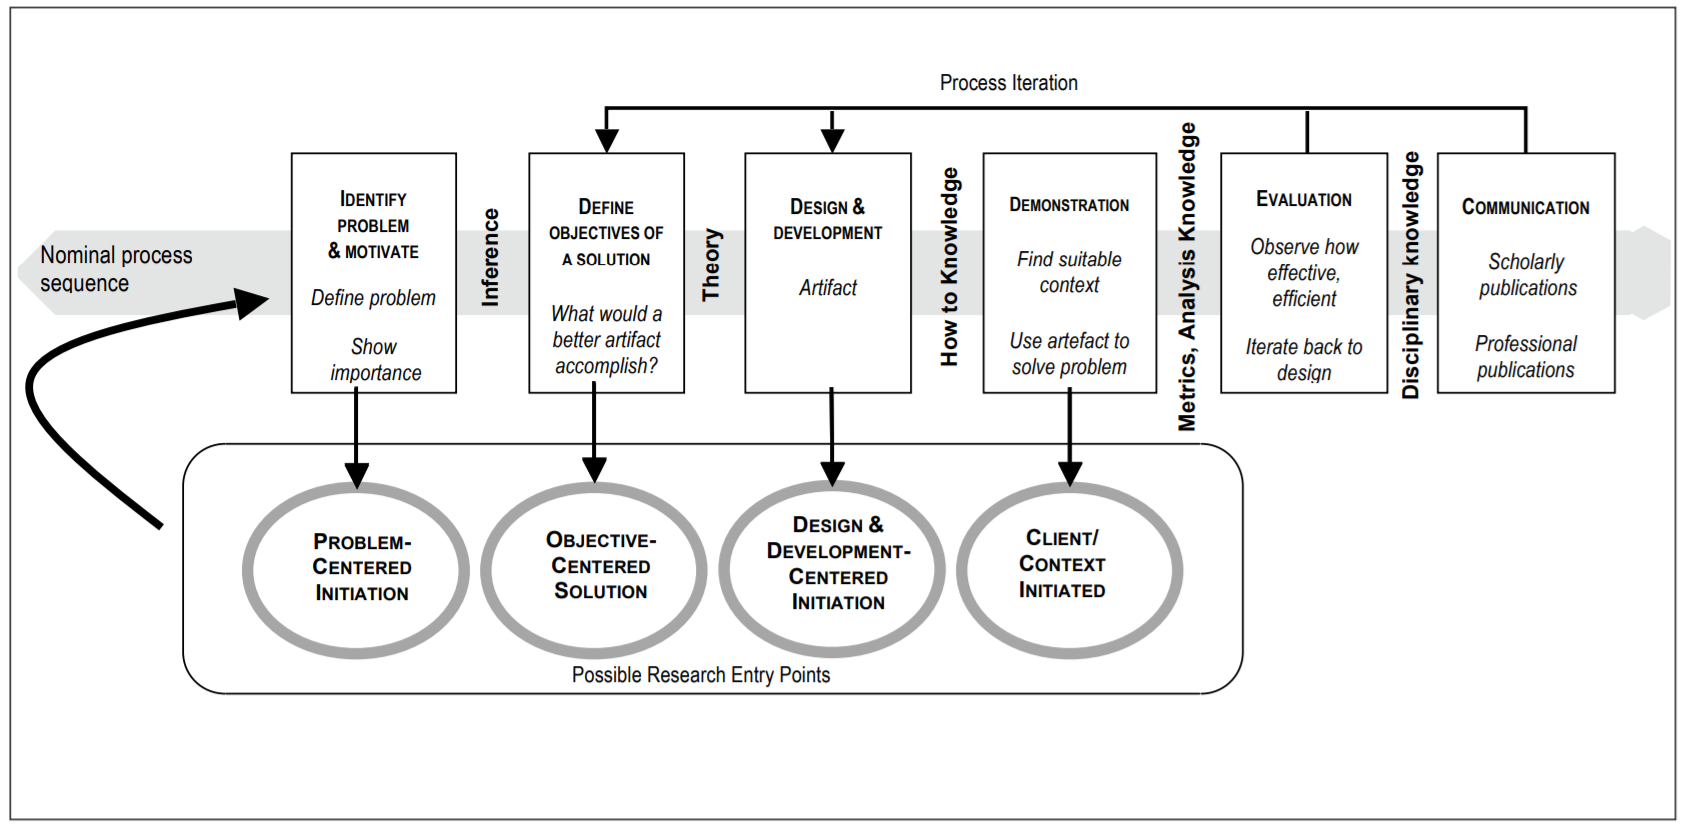
\includegraphics[width=\linewidth]{figures/DSRMPeffers.PNG}
    \caption{Design Science Research Methodology, ~\cite{Peffers2007}}
    \label{fig:DSRMPeffers}
\end{figure}

\subsection{Problem identification and motivation:} 
The process of identifying vessels with an abnormal behaviour, is a complex task. This is mainly because in vessels, abnormal behaviour can be caused by numerous different causes.
  
The authors ~\cite{Laxhammar2008} define Anomaly Detection (AD) as "a method for separating an often in-homogeneous and hard characterized minority of data from a more regular majority of data, by studying and characterizing the majority, so that data in the minority appears as deviations from the patterns found in the majority". 

The main focus of this work is the research and develop of methods that represent vessel motion data, in ways that anomalies can be found.

The MARISA project involves 22 organizations completely motivated to fulfill the overarching objective. 

With the current needs of a more comprehensive approach at the European seas, new and more efficient methods that promote the information exchange between European Union countries, optimizing the European maritime area surveillance and its maritime borders are a current need.

The MARISA project is funded under a H2020, which is a financial instrument that promotes innovation through the European Union.

\subsection{Define the objectives for a solution:}
The research problem is defined accordingly with the MARISA project, which can be defined as: 

~\textit{How to create a system that fuses Data from different sources, capitalizing on the large amount of unexploited maritime data, while autonomously identifying Anomalous Vessel Behaviour.}  

Due to the complexity of this main question, it's important to divide it into smaller questions:

\begin{itemize}
\item Which sources are the most viable to gather spatial data from Vessels,
turning it into a sound Data-Set?
\item Which techniques can transform Spatial Data into Sequential Data, thus creating Vessel trajectories?
\item Can previous Algorithms mine trajectory data from AIS sources, finding anomalies?
\end{itemize}

\subsection{Design and development:} In order to achieve the proposed goals and simultaneous contribute to the MARISA project, the two following objectives were created in Design Science Research. These objectives are described as artifacts:

\begin{itemize}
\item \textbf{Data-Set} A solid Data-Set must be gathered and cleaned. Through the MARISA project, the process of obtaining a Data-Set can be prolonged.Thus ways of obtain AIS Data-Sets free of cost must be researched.

\item \textbf{Route Definition} Numerous methods of vessel route definition, are presented in ~\ref{chapter:literatureReview}.
Although, at this moment a method was chosen that represents the route as a whole. Therefore no information is lost. A detailed description of the latter is presented in ~\ref{section: Trajectory Analysis}.
\end{itemize}

\subsection{Demonstration}https://v2.overleaf.com/project/5b094c27dd648c7b207643b4
While the first artifact is a necessity for future work, is on this data-set that future work will be developed. At this moment I'm using a data-set, from the North America region that has 3.3 million AIS messages from various vessels.
All the MARISA requirements, will in an initial phase be developed on this data-set.
\subsection{Evaluation}
The evaluation of the future artifacts, will be firstly conducted by INOV and after by MARISA partners.
Performance assessment of the artifacts, will be considered after the first implementation is concluded.

\subsection{Communication} 
The research is being conducted for the fulfillment of my masters, therefore a dissertation will be presented for the final evaluation. There is the possibility of submitting future articles for publishing, this possibility depends on the MARISA project.

\chapter{Literature Review}
\label{chapter:literatureReview}
\lhead{Chapter 2. \emph{Literature Review}}

Objectives for the MARISA project are well defined. In order to achieve the proposed goals and in preparation for this thesis a vast number of subjects were investigated. An investigation in the following theoretical topics : behaviour analysis, anomaly detection and maritime safety technologies, were the major keywords for this literature review. 

In section \ref{section: Similar Frameworks} an analysis of the principal similar Frameworks found in the Literature, will be presented.
 A brief introduction to the maritime domain, regarding the Maritime Safety affairs is presented in section \ref{section: Maritime Safety}. In subsection ~\ref{subsection: chp2_AIS}, a description of the AIS technology and its use in the Maritime domain is presented.

\section{Maritime Safety}
\label{section: Maritime Safety}

Shipping is most likely, the most international task of all Worlds Industries, because of this international nature. It has long been recognized that improving maritime safety, is more effective if it is  carried out on a international level, than by individual countries acting unilaterally without any co-ordination, ~\cite{IMO2016}.

The UN (United Nations) in 1948, established the International Maritime Organization (IMO), as the first and principal international organization devoted to maritime matters. 

Since it's creation, the IMO has promoted the adoption of 50 conventions and protocols. The IMO has adopted more than 1000 codes and recommendations regarding the maritime safety and security.

The IMO objectives are easily summarized into their slogan : safe, secure, and efficient shipping on clean oceans.

\subsection{Automatic identification system (AIS)}
\label{subsection: chp2_AIS}
While the maritime safety domain is a vast and complex field for this investigation, it is important to focus on the technologies that the maritime domain has presented.

Automatic Identification System (AIS) is used to identify and locate Vessels by electronically exchanging data over high frequency VHF radio bandwidth to, other nearby ships and Vessel Traffic Services (VTS) stations.

The main motivation for the adoption of the AIS was its autonomous ability to identify other Vessels assisting humans with the collision avoidance. It has the ability to detect other equipped Vessel in situations where the radar detection is limited such as around bends, behind hills, and in conditions of restricted visibility by fog, rain, etc, ~\cite{Harati-Mokhtari2007}. 

In 2000, the IMO adopted a new requirement for all ships, to carry an automatic identification system (AIS) that automatically provides the Vessel information to coastal authorities and other Vessels.

This regulation was initially imposed for all international ships with 300 gross tonnage or more and for ships with 500 gross tonnage and upwards navigating not international voyages. After 31 of March 2014 all EU fishing Vessels above 15m, are obliged by the European Commission to install an AIS, ~\cite{EC2018}

The ships information sent over the AIS is classified into three main categories, they are presented in table:
\begin{table}[H]
\centering
\caption{AIS Information Description}
\label{Table: AIS Categories}
\begin{tabular}{|l|l|}
\hline
\textbf{Category} & \textbf{Description} \\ \hline
 & MMSI - Maritime Mobile Service Identity \\ \cline{2-2} 
 & IMO number \\ \cline{2-2} 
\textbf{Static Information} & Call sign and name \\ \cline{2-2} 
 & Type of ship \\ \cline{2-2} 
 & Length and beam \\ \cline{2-2} 
 & GPS Antenna location \\ \hline
 & Draught of ship \\ \cline{2-2} 
\textbf{Sailing Related Information} & Cargo information \\ \cline{2-2} 
 & Destination \\ \cline{2-2} 
 & ETA - Estimated Time of Arrival \\ \hline
 & Position of the ship \\ \cline{2-2} 
 & UTC - Coordinated Universal Time \\ \cline{2-2} 
 & COG - Course Over Ground \\ \cline{2-2} 
\textbf{Dynamic Information} & SOG - Speed Over Ground \\ \cline{2-2} 
 & Heading \\ \cline{2-2}
 & Navigational Status \\ \cline{2-2}
 & Rate of turn \\ \hline
\end{tabular}
\end{table}

Each Vessel transmits specific information related to the Vessel itself, the MMSI represents a 9 digit unique ID number, that every Vessel is assign with.
Most of the information sent over AIS, is automatically generated by the ships sensors such as the GPS and the compass. Thus minimizing the possibility of manipulate this data, although there is still information that is manually inserted by the crew such as the Navigational Status and the Heading.

Ships fitted with AIS are obliged to maintain the AIS in operation at all times. The AIS autonomously broadcast information, every certain time interval, therefore ships ping their AIS information every time interval   There are international agreements, that protect the navigational information.


\section{Behaviour Analysis}
Behaviour Analysis, is a vastly researched topic that involves many research fields. A vast number of Frameworks with the main objective of Maritime Behaviour Analysis are proposed in the literature, some of these frameworks are presented in section ~\ref{section: Similar Frameworks}.

For this work Vessel behaviour is as considered as a baseline in which abnormal behaviour can be found. This baseline occurs as normal trajectories are various and constant, producing a normalcy model of Vessels dynamics in which Machine Learning Techniques can learn.

Anomalies don't necessarily mean that there is something abnormal with the ship Vessel behaviour. That is something hard to imply with only AIS data. Anomalies in the AIS data can represent numerous abnormal events. Some of them that can be illegal, that's why further investigation from maritime authorities is needed. 

\subsection{Similar Frameworks}
\label{section: Similar Frameworks}

There are a vast number of frameworks in which Vessel behavior will be analyze. This will be done with the purpose of anomaly detection which are fully defined as integrated systems. The authors in ~\cite{Lei2016} suggested the framework MT-MAD (Maritime Trajectory Modelling and Anomaly Detection), in which a given set of moving objects, the most frequent movement behaviour are explored, evaluating a level of suspicion hence detecting anomalous behaviour.

The authors in ~\cite{Pallotta2013}, introduced the framework TREAD (Traffic Route Extraction and Anomaly Detection). The framework is proposed in which an Unsupervised Route Extraction is used to create a statistical model of maritime traffic from AIS messages, in order to detect low-likelihood behaviours and predict Vessels future positions.

A framework for Vessel behaviour analysis focusing on Vessel interaction or rendezvous. The proposed framework, is divided into the following three logical connected phases: Engagement Detection, Scenario  Detection and Anomaly Detection. The use of the 3-phase framework serves as a filter to reduce the volume of data that is processed by the sub-sequential phase. Therefore prioritizing critical scenarios, that request human intervention ~\cite{Shahir2015}.

Although accessing the performance of the frameworks, is an ardours task. There is no defined benchmark set where tests can be performed, with labeled samples described as positives or negatives of what are considered anomalies at seas ~\cite{Laxhammar2008}. 

In~\cite{Mao2016}, a detailed solution for constructing an AIS database, with the potential value for being used as benchmark database for maritime trajectory learning, and efficiency testing of data mining algorithms.

A partition-and-detect trajectory in which trajectories are partitioned into a two-level of granularity achieving high efficiency and high quality trajectory partitions, therefore detecting outlier trajectories using density-based methods, ~\cite{Lee}.

There are numerous studies that show how, Vessels tend to alter their routes in order to achieve safe distances when passing near other Vessel. In ~\cite{2017Offshore} a detailed study on Merchant Vessels AIS data, presents how this type Vessels alter their route, when new surface offshore petroleum installations are constructed.

\section{Trajectories Analysis}
\label{section: Trajectory Analysis}
Trajectories analysis is a researched field for numerous years. It is researched in areas where moving objects, this objects can be Humans, vehicles, animals, or even natural events such as hurricanes or storms.
A survey of trajectory data analysis applications, is presented in ~\cite{Feng2016}.

As the volume of positional AIS data exponentially increasing, it is important to find methods in witch raw trajectories data can produce value. This methods that learn with trajectory data can greatly impact the Maritime domain.

Trajectory learning is the process of learning motion-patterns from trajectory data using unsupervised techniques, mainly clustering algorithms ~\cite{LeGuillarme2013}.
Morris and Trivedi ~\cite{Morris2008}, further categorize trajectory learning as a three-step procedure: 

\begin{enumerate}
\item Trajectory Pre-Processing.
\item Trajectory Clustering. 
\item Path Modelling.
\end{enumerate}

In the Maritime domain, as Vessels are free to navigate in open waters, this fact produces a specific level of uncertainty related to Vessel trajectories, there are no standards for Vessel trajectory representation.

A way to discretize a trajectory discovering frequent regions is presented in ~\cite{Lei2016}. Representing the trajectories in a spatial grid in which a cell represents a geographical area with a defined size.

Pallotta, proposed a method that enriches the raw Vessels tracks with a description of the ship movements. This is the raw trajectories are labelled with the Vessel movement type information as 'Stationary' or 'Sailing' ~\cite{Pallotta2013}.

The authors in ~\cite{Lee}, raw trajectories are partitioned into sub-trajectories, creating a new insight for data analysis, adding the possibility of focused region analysis.  

A framework for scene modelling using trajectory dynamics analysis, for the discovery of POIs(Point of Interest) and the learning of AP(Activity Path), ~\cite{Morris2008}. 
These last representation is quite important for the Maritime domain, as the discovery of new POIs, can indicate the common Vessel destinations (e.g. frequent fishing zones, ports, etc.).  

\section{Time Series}
\label{section: Time Series}
The concept of time series is related to trajectories, as a time series is a set of ordered observations on a a quantitative characteristic of a
phenomenon at spaced time period, ~\cite{Ivanovic2016b}. Formally, a uni-variate time series $xj$, is defined as a sequence of real numbers, where $n$ is the length of the series, represented as:

\[xj = \left \{ x(i) \in \mathbb{R}: i = 1,2,3,...,n \right \} \]

 There are numerous applications for time series analysis, one of the main applications, is the use past time series, in order to forecast future values. These applications are used in numerous areas such as economics, engineering and others.


\subsection{Multivariate Time Series}
The AIS data cannot be described as a uni-variate times series, as it is composed by various variables. Therefore AIS data needs to be analyzed as a Multivariate Time Series (MTS).
For each AIS message, the features can be extracted with the timestamps that the message was broadcast. A detailed description of the AIS features is found in section ~\ref{subsection: chp2_AIS}. 

A possible representation of a Multivariate Time Series, $X$ is:
\[ X = (x_{1}, x_{2}, x_{3}, \cdots,x_{m}) \]

Where each $xj$ is defined in section ~\ref{section: Time Series}.

\[ Xj = \left \{ Xj(i) \in \mathbb{R}: i = 1,2,3,...,n \right \} (j = 1,2,3) \]

The analysis and classification of MTS is a arduous task for traditional machine learning algorithms, mainly because these algorithms do not handle well dozens of variables, ~\cite{MTS1}. Representing MTS into multiple univariate time series, can create losses in the correlation of these variables, as variables are being processed them independently.

\subsection{Time Series Clustering}
Temporal data mining research, a big emphasis lies on the clustering, and posterior classification of time series data. Time Series Clustering is used to identify in data-sets, homogeneous groups where same group object similarity is maximized, and the minimized when not in same group.  

The authors in ~\cite{WarrenLiao2005}, summarize previous work that investigates the clustering of time series applications in various fields, and propose an extensive survey. 

The same authors, define a necessity to clustering, when working with unlabelled data. This data can come from various sources including : categorical, numerical, images, spatial, e.t.c.

The main source of data for this work is AIS data, which is a  unlabelled multivariate data source. Labelled AIS data-sets for anomaly detection are either really expensive, or just not available for the public domain.  


\begin{figure}[H]
	\centering
	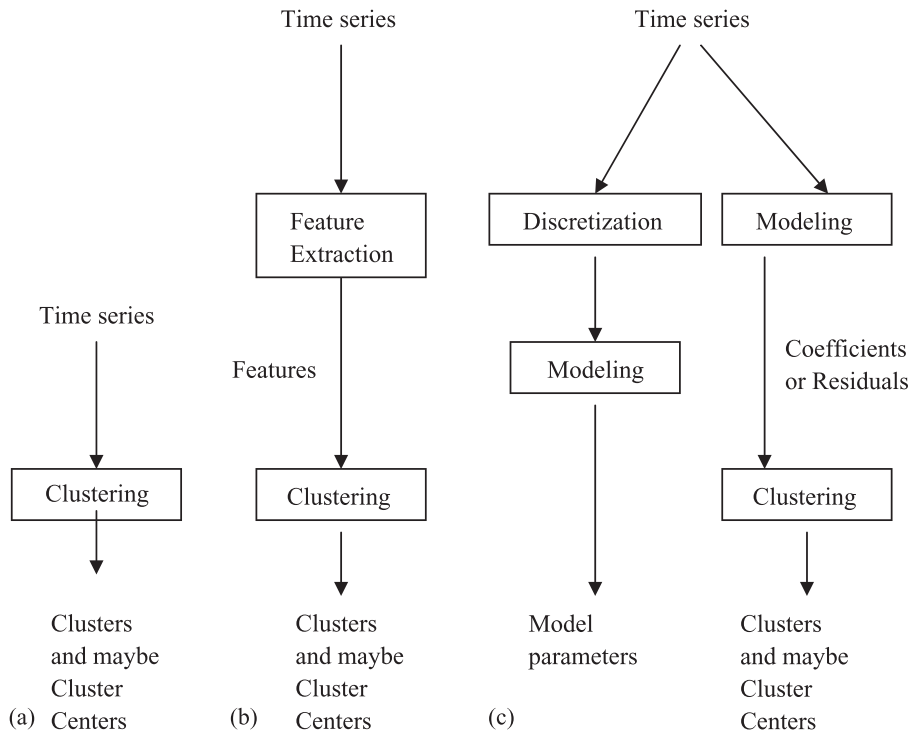
\includegraphics[scale = .6]{figures/TimeSeriesClustering}
    \caption{Three types of time series clustering defined in, ~\cite{WarrenLiao2005}}
    \label{fig:TimeSeriesClustering}
\end{figure}

Time Series Clustering can be categorized into three main general approaches, simply described in figure ~\ref{fig:TimeSeriesClustering}, these categories being:

\begin{itemize}
\item \textbf{Raw-data-based approaches (a)} These approaches work with raw sets of data, normally in the time domain. 

\item \textbf{Route Definition} Several methods of Vessel route definition, are presented in~\ref{chapter:literatureReview}.
Although, at this moment a method was chosen that represents the route as a whole. Therefore no information is lost, a detailed description of the latter is presented in~\ref{section: Trajectory Analysis}.

\item \textbf{Model-based approaches} This is a more complex clustering technique, in which, each Time-Series is considered as a statistical model or as a mixture of statistical distributions, thus two time series are considered similar when the models that fit this distributions are similar. 
\end{itemize}


%\todo{Needs completion for future work.}


\subsection{Time Series Classification}
Time series classification, is used for numerous purposes, from, the main difference when classifying or clustering Time Series lays in the fact that, classification can occur when a predefined set of classes already exist and the main objective is to classify this data in the different classes, thus in machine learning being considered a Supervised Learning task. 

Early work, from 1998, the authors propose p-value hypothesis test, performed for every pair of stationary multivariate time series, ~\cite{MTS1999}.

Three main categories of sequence time series classification, are defined by the authors in ~\cite{MTS_Classification}:

\begin{description}
\item[Feature Based Classification] A sequence of features is transformed into a feature vector, then convectional classification methods are applied. Feature selection represents is an important task for this method of classification.

\item [Distance Based Classification] The distance function that measures the
similarity between the time series, induce the quality of the classification overall. A more detailed research on these distances is presented in \cite{Knorr2000}.

\item [Model Based Classification] Where models, such as multivariate Gaussian mixture model (GMM) ~\cite{Laxhammar2008}, Support Vector Machines (SVM) or Hidden Markov Models (HMM) and other statistical models are used to classify time series.

\end{description}
 

\section{Distances Measures}
In order to compare classify a time series using distances, the concept of distance, and type of distance must be defined.

A distance is defined as a numerical measurement, that measures how far two objects are from each other. There are a vast number of distances used in computer algorithms. The most commonly used distance measure is the Euclidean distance, this measurement is a metric distance function, since it obeys to the three fundamentals metric properties: non-negativity, symmetry and triangle inequality ~\cite{Cai2004}. 

The similarity between two time series, can be calculated by simply summing the ordered point-to-point squared distance between both time series, this is shown in figure ~\ref{fig:EuclidianDTW}. 

Although, euclidean distance between two time series can only be calculated if, both time series are of equal length, ~\cite{EuclidianRef}. 
If two time series are identical, but one is shifted slightly along the time axis, using the Euclidean distance, it may consider the time series very different from each other, ~\cite{Salvador2007}.

This creates a problem when analyzing certain type of time series, as both may not have them same length, or might just be time-shifted, which happens when analyzing AIS data. In the literature a few solutions are presented, one of them is using another distance measure. 

\begin{figure}[H]
	\centering
	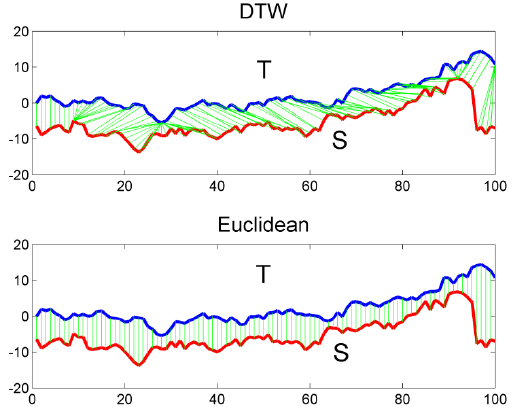
\includegraphics[scale = .5]{figures/DTWEuclidean.png}
    \caption{Difference between DTW distance and Euclidean distance (green lines represent mapping between points of time series T and S),~\cite{EuclidianRef}}
    \label{fig:EuclidianDTW}
\end{figure}


\subsection{Dynamic Time Warping (DTW)}
Dynamic Time Warping (DTW) is a algorithm that computes the optimal alignment and distance between two time series, ~\cite{Seto2015}. One time series may be “warped” non-linearly by stretching or shrinking it along its time axis.
%[GET A BETTER REF FOR THIS, NOT SALVADOR].

Although computing the DTW between two time series, is quite computationally expensive, has it's time and space complexity is $O(N^2)$, that limits its usefulness to only small time series with no more than 1000 points, ~\cite{Salvador2007}. 

As distance measures play an important role for similarity problem, in data mining tasks.








%\section{Data Fusion}
%\todo[inline]{Needs completion for future work. Depending on future work this might be needed.} 




\chapter{Modular Anomaly Detection Framework}
\label{chapter:Chapter 3}
\lhead{Chapter 3. \emph{Methods and Systems Developed}}

In this Chapter, we present the overall description of steps towards the development of the \emph{Modular Anomaly Detection Framework} which is be used throughout this dissertation. 
A crucial component in this work relied on a technically accurate definition of a \emph{maritime anomaly}. This is generally speaking a challenging task since a data-driven definition is currently lacking or insufficient. A more meaningful solution to this problem was provided by the aid of maritime experts who were engaged in the \textsc{Marisa} project. In particular, members of the Portuguese Navy interacted with us in order to offer the required their exclusive technical insight.

Given their specific input and real-world knowledge of the maritime domain, one can arrive at a well-defined concept of anomaly that can be translated into a precise notion to be used in this Framework. Before we engage in the specific requirements that served as a blueprint for the developed framework, such a definition will be given. This will then be followed by the technical description of such requirements, namely by distinguishing \emph{anomaly} and \emph{data requirements}.

Lastly, a general overview of the proposed Modular Anomaly Detection Framework, which will be referred to as MAD-F from now on, is presented. This is done in light of Figure~\ref{fig:Framework}, whose modules are explained individually throughout the following Subsections~\ref{subsection: Data Ingestion},~\ref{subsection: 3 Pre-processing},~\ref{subsection: 3 Feature Engineering}, ~\ref{subsection: 3 Vessel Trajectory Extraction},~\ref{subsection: 3 ADS} and~\ref{subsection: 3 RB-ADS}.


\section{Anomalies within the MAD-F}
\label{section: Framework Requirements}
An anomaly may have numerous interpretations depending on the context in which it is found. However, it can be generally conceptualised as a subset of data that stands out in some preconceived way when contrasted to the overall dataset. Nowadays, the anomaly detection of vessel behaviour is solely done by human maritime experts. This procedure depends on national security agencies. Within their duties, these agencies are responsible for assuring the coastal surveillance of their territory by assessing possible threats and identifying abnormal behaviour. The current methods employed by these institutions are neither efficient nor scalable and therefore not suitable for the challenges brought by the exponential growth of vessels at seas. This state of affairs creates an ideal situation for the use of data-driven models to assist the maritime experts.

The notion of anomaly just presented is unsatisfactory given both the complexity and purpose of the problem. For the goals of this project, such a technical definition is tailored specifically by the maritime agencies involved in the \textsc{Marisa} project and we therefore refrain from applying our own definitions, which usually stem from abstract statistical data-driven notions. 

By having meetings with maritime experts a list of the anomaly requirements was agreed. For this work this list served as not only the concrete anomaly requirements, but also as a guide for the overall implementation of the \emph{MAD-F}. The list of anomaly requirements in shown under in Table~\ref{Table: Anomaly Requiremtens}.

\begin{table}[H]
\centering
\caption{MAD-F anomaly requirements, which were defined by maritime officers.}
\label{Table: Anomaly Requiremtens}
\begin{tabular}{@{}ll@{}}
\toprule
Anomaly Requirement & Provided Description \\ \toprule
\textit{\textbf{AR1}} & \begin{tabular}[c]{@{}l@{}}Detect Abnormal changes of \\ (more than a configurable value) Direction.\end{tabular} \\ \midrule
\textit{\textbf{AR2}} & \begin{tabular}[c]{@{}l@{}}Detect Abnormal changes of \\ (more than a configurable value) Velocity.\end{tabular} \\ \midrule
\textit{\textbf{AR3}} & \begin{tabular}[c]{@{}l@{}}Detect Vessels disappearance from sensor \\ coverage for more than a configurable Time Period.\end{tabular} \\ \midrule
\textit{\textbf{AR4}} & \begin{tabular}[c]{@{}l@{}}Detect when the observed \\ Vessel Navigational Status is not consistent \\ with the reported Vessel Kinematic features.\end{tabular} \\ \midrule
\textit{\textbf{AR5}} & \begin{tabular}[c]{@{}l@{}}Detect when Vessels report a \\ geographical and time incompatibility.\end{tabular} \\ \midrule
\textit{\textbf{AR6}} & \begin{tabular}[c]{@{}l@{}}Detect when two or more Vessels are \\ approaching close to each other.\end{tabular} \\ \bottomrule
\end{tabular}
\end{table}

As mention previously, requirements for this work were distinguished from anomaly requirements and data requirements. The latter was intrinsic for this work, as the uncertainty of data types and sources when dealing with the maritime field is immense. The problem of having numerous types and sources of data is still aggravated as the maritime domain is also capable to produce enormous workflows of data. Thus, a specific data requirement for this work could be simply specified as: 

\emph{The developed Framework, must be able to ingest fuse and store different sources of maritime Data, while also handling enormous workflows of data in real-time.}

\section{Modular Vessel Anomaly Detection Framework}
In order to develop a Framework capable of achieving the requirements defined above in Section~\ref{section: Framework Requirements}, we propose the Modular Vessel Anomaly Detection Framework. The \emph{MAD-F} is able to ingest data from different feeds in real-time data while simultaneously constructing a Data-Base for Vessels Trajectories in a unsupervised manner. Anomalies are then detected in a offline manner from the saved trajectory data, or online in real time addressing the incoming streams of Vessel Data. 
The framework was developed to be modular as there are either no inputs or outputs standards for the Maritime Domains. Thus, by providing a configurable and not static framework, we give the configuration flexibility for the \emph{MAD-F} being configured for different scenarios or even different National Maritime Authorities, or even to new Modules being added in the future.
In Figure~\ref{fig:Framework} we present the architecture of the \emph{MAD-F} and the following subsections will discuss each of the framework modules: Data Ingestion, Data Pre-processing, Feature Engineering, Trajectory Extraction and both anomaly detection modules : Anomaly Detection Service and Rule Based Anomaly Detection Service.
\begin{figure}[H]
\centering
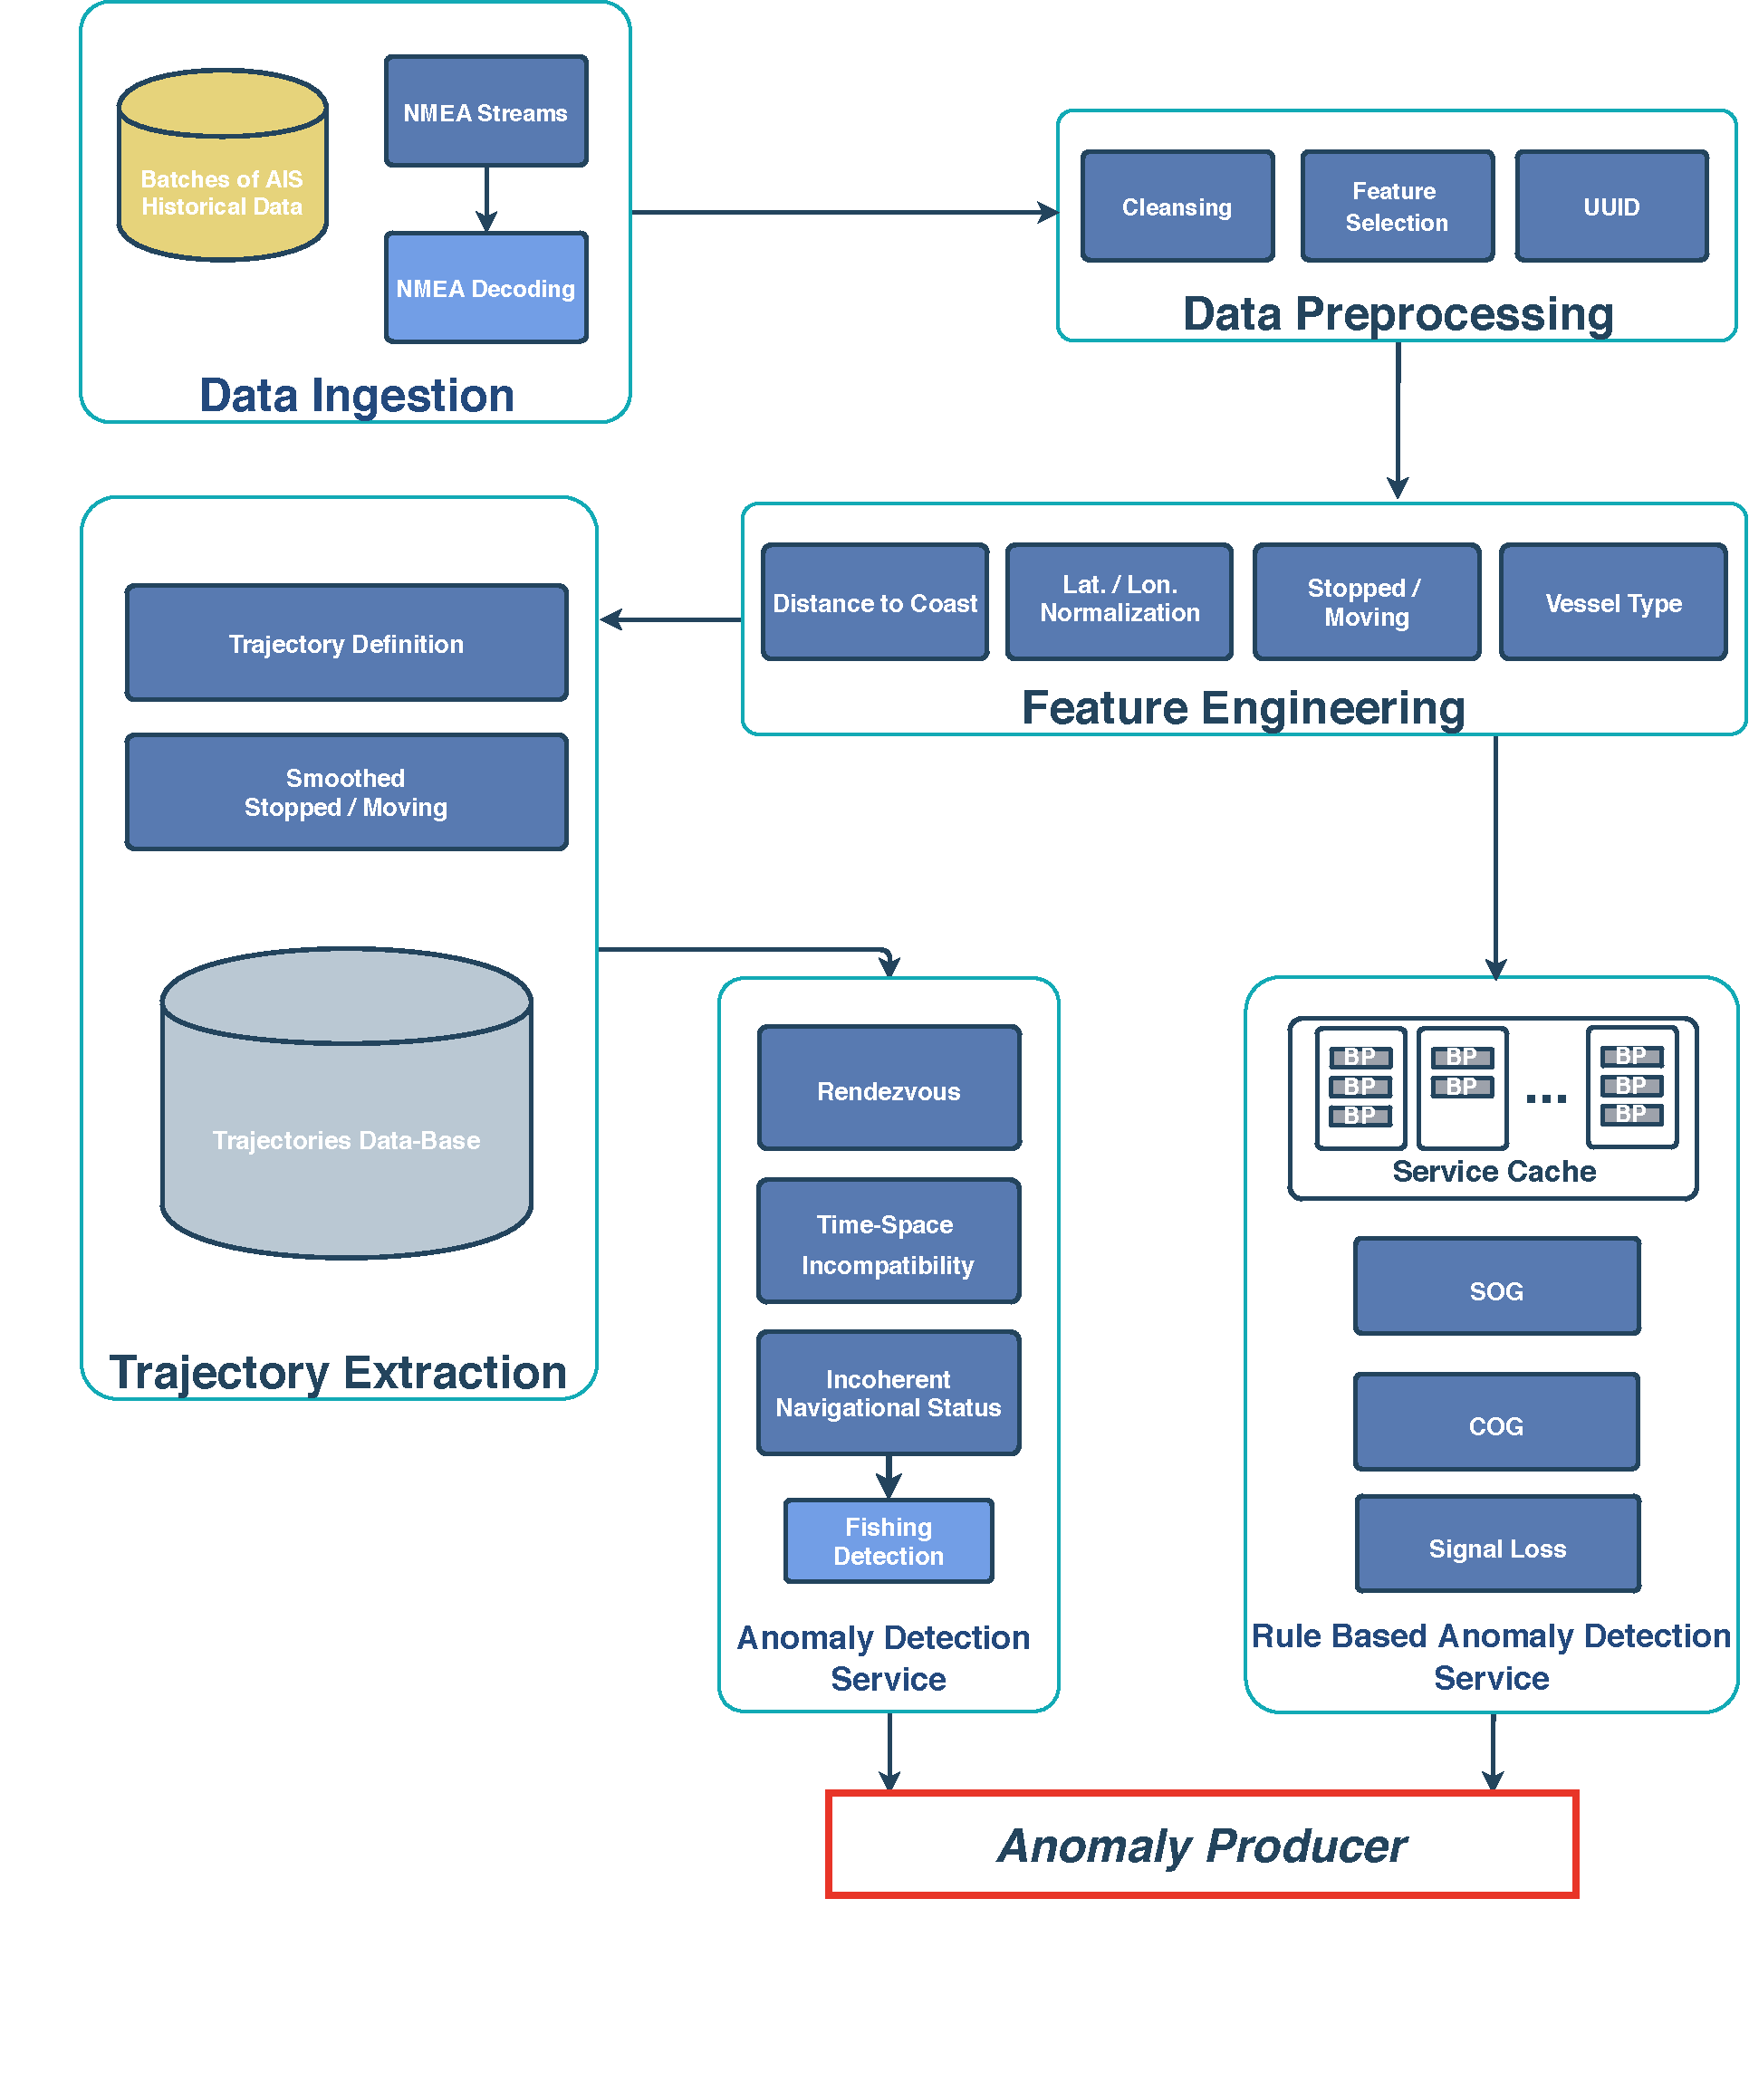
\includegraphics[width=\textwidth]{figures/Ch3/Framework.pdf}
\caption{Proposed architecture for the \emph{MAD-F} Framework}
\label{fig:Framework}
\end{figure}

\subsection{Data Ingestion}
\label{subsection: Data Ingestion}
Data Ingestion Module, represents the Data input for the developed Framework. AIS data was the most representative data type used for this work, as it showcases the actual instantaneous Vessel information.
Although, used AIS data for this work came in two really distinct formats. It came either in \emph{Historical Batches} representing Historical sets of Data, or real \emph{NMEA AIS Streams} which represent real, real-time data. For both data formats, the framework is scalable, and able to ingest one or multiple feeds / sources of data simultaneously.

%AIS Historical Data-Sets, can be found in open-access repositories, although Historical AIS Data providers cap the frequency of the messages transitions. This drastically reduces the number of transmitted messages, but also reduces the overall detail of the Data, as lower transmissions rates produce a less certainty of the movement presented by each Vessel. Which, for most general uses of AIS (e.g. managing a fleet, estimations of time of arrival ...), transmissions rates of 3 Seconds vs 30 Seconds, do not provide any information gain, as Vessel kinematics tend to not change abruptly in short periods of time. 

Via the \textsc{Marisa} project, we accessed AIS live feeds from antennas all around the Portuguese coast line. This Antennas receive Vessels transmissions via AIS up to 20 Nautical Miles of the shore depending on the weather conditions, and with reception rates up to 30 Messages per minute per vessel. The real live feeds of AIS data, are received via TCP in the NMEA format.

National Marine Electronics Association (NMEA) is a standard communication protocol used by Maritime Sensors such as Accelerometer, Giroscope, GPS receivers, etc.
NMEA encapsulates the information from the different Vessel sensors, and broadcasts this information to coastline antennas and nearby Vessels via AIS protocol.

\begin{figure}[H]
\centering
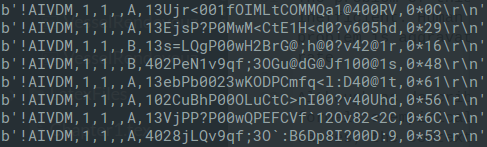
\includegraphics[scale = .55]{figures/Ch3/NMEAexample.png}
\caption{Snapshot of raw AIS data in NMEA format.}
\label{fig:NMEAexample}
\end{figure}
%Via the project, we had access to multiple live NMEA feeds, as a way to not only validate our developed methods with live feeds of Nautical data, but also to produce methods that were capable of handling the scale of data that is produced by National feeds.
Although the use of real AIS data comes with many challenges, as it is mandatory to decode, sort and store the received data, thus allowing the incoming data to be used as viable source of data. Secondly, as AIS-receiving stations receive the broadcast AIS information from multiple AIS-equipped vessels simultaneously, and the reception range of each AIS-receiving can vary depending on the actual weather conditions and the location of where such station is located. This originates two main problems :
\begin{enumerate}
\item Duplication of reception:  With the variation of reception ranges from the AIS-receiving stations, this creates the problem of multiple stations receiving the same vessel broadcast. The duplication of messages is a problem which occurs when handling real NMEA streams, the methods used to solve such problem are presented in Section~\ref{subsection: ch4 Data Ingestion}.

\item Non-reception of broadcast: Similar to the problem presented above the non-reception of by any receiving station can also occur. To address this problem, Maritime Agencies use satellite AIS (S-AIS). S-AIS solves the problems related to the reception range, but presents another problem with refreshment rates, has the reception of the broadcast are dependent of satellite revisit time \cite{Robards2016ConservationReview}. 
\end{enumerate}


%when dealing with real-time NMEA feeds as
%the reception range of the AIS receiving antennas varies depending on weather condition when this antennas receive information from multiple Vessels two more common problems can occur:


%. Normally, AIS-Receiving stations are antennas located along the coast line in high grounds, the reception range of these antennas vary, mainly depending on distance to shore, the elevation in which the antenna is located, and the antenna type itself.

%Although, the distance in which Stations are capable of receiving AIS messages presents a problem to the Data, as reception ranges vary from 15 Nautical Miles to 50 Nautical Miles, which creates the problem of 



%\subsection{Data Storage}
%With NMEA streams producing enormous workflows of data, the storage of becomes a problem for the developed Framework, as it must not only decode and process the NMEA feeds but also store the decoded messages, in a "very fast" and scalable way.

%Thus, and as requirement of the MARISA project was to use Apache Spark [REF FOR APACHE SPARK] modules for data-ingestion and pre-processing, we decided to use Apache Cassandra as the Data-Storage for the proposed framework.

\subsection{Data Pre-processing}
\label{subsection: 3 Pre-processing}
The Data Pre-processing module, is the first step of Data Wrangling in our Framework, the motive for this module is to select, transform, and clean the received data, incoming from the Data Ingestion Module. 
As described in Section~\ref{subsection: chp2_AIS}, AIS presents a large amount of different features, which can be used for different problems. Feature Selection represents a important step for this work. This work being partially a unsupervised learning problem, the selection of the "relevant" features directly influences the overall performance of the \emph{MAD-F}, but also the expected results from the learning task. Such representative task requires pre-conceived knowledge of Vessels dynamics and behaviour, which is only gained with experience in the Maritime Domain. For this work the feature selection was done based on the literature, and also by accessing Maritime Expert Knowledge via the \textsc{Marisa} project.

During the \emph{Pre-processing}, a data-cleaning process is conducted, discarding corrupted data. This is done based on the information that standardises the AIS features, which is further detailed in Section~\ref{section: Data Analysis}.

Most importantly, in this module the concept of \emph{Behavioural Point} is defined. \emph{Behavioural Point} which will be referred as $BP$ from now on, for this work represents our normalised representation of the previously selected features. A detailed explanation of this concept is provided in Subsection~\ref{subsection: Behavioural Point}.

\subsection{Feature Engineering}
\label{subsection: 3 Feature Engineering}
Feature Engineering, represents the second step of Data Wrangling for the proposed Framework. During this step, the already pre-defined $BPs$, in the Data Pre-processing module, are enriched by extrapolating additional features. 

Firstly for each $BP$ received by this module, if the Vessel Type is not received in the AIS message, the Vessel Type is either extracted from external Vessel Information Sources, or it is scrapped from this internet.
Secondly, each $BP$ is enriched with by calculating the closest country and respective distance to Shore. The same is done to Ports, by calculating the distance to the closest Port. Also, in this module with the reported kinematic features, the instantaneous move state of the vessels is inferred.

This procedures are further individually explained throughout Subsections~\ref{subsection: Vessel Type},~\ref{subsection: Distance to Coast},~\ref{subsection: Stopped/Moving}.

%presents a crucial step for any machine learning project, as 

%selecting the right features to represent the data, directly influences any result generated by the Anomaly Detection Modules.  

%We further enrich our features in two ways, firstly by analysing each AIS message as a single point in Time and calculating additional distances, such as distance to Shore and distance to the most near Port.

%each point in t the represented features of each message by by doing a point based analysis, in which we considered the information of  

%by normalizing the Latitude and Longitude features of each position, calculating the Distance to Shore and the kinematic features that represent the instantaneous move-state of the Vessel. Every calculation is done a priory, thus enhancing the performance and reliability of the Anomaly Detection Modules, which are explained in detail in section \todo{REF TO SECTION!}

\subsection{Vessel Trajectory Extraction}
\label{subsection: 3 Vessel Trajectory Extraction}

Vessel Trajectory Extraction module, handles the definition, storage,  updating and inserting of new incoming $BPs$ into defined \emph{Trajectories}.
When considering Trajectories, the $BPs$ stop being valued as single points in Time, and the aggregation of $BPs$ via the Vessel Identifier throughout time, start representing a Vessel Trajectory. This allows a more conclusive Vessel behaviour analysis based on its past trajectory. Although, in order to work with Trajectory, such concept needs to be defined and represented in a optimal manner. Furthermore, when dealing with real Maritime data (and specially when working with real Maritime Authorities) it is extremely important to trace-back/log of the data, from which, justifying generated anomalies is possible. 
In Section~\ref{subsection: Trajectory Definition} our definitions of a vessel trajectory. 

%Behaviour analysis based on the past historical Trajectory data. Analysis of Trajectories drastically increases the level of complexity, when compared to analysis points, thus it is required quick and efficient representation of a Trajectory.

\subsection{Anomaly Detection Service}
\label{subsection: 3 ADS}
ADS (Anomaly Detection Service) Module, represents for our Framework the Batch Layer for Anomaly Detection Services. \emph{ADS} module works offline in effective time, on batches of historical Trajectory Data served from \emph{Trajectory Data-Base} from the \emph{Trajectory Extraction} module. Access to Trajectory Data, is done by querying the \emph{Trajectory Data-Base} with a configurable set of parameters, which can be time restrictive(such as the 10 past Hours) and or from a Vessel specific set of Vessels. 

Received Trajectory Data, is then used to detect: \textbf{Time Space Incompatibility}, \textbf{Vessels Rendezvous}, and \textbf{Incoherent use AIS Navigational Status}. For the latter, we create a sub-method for the detection of \textbf{Fishing Activities} based on Vessels characteristics and Dynamics and the reported Navigational Status.
The implemented methodology for the detection of each Anomaly is represented in Subsections~\ref{subsection: 4 Time-Space Incompatibility},~\ref{subsection: 4 Navigational Status Validation},~\ref{subsection: Fishing Activity Detection} and~\ref{subsection: 4 Vessel Rendezvous} respectively.


\subsection{Rule Based - Anomaly Detection Service}
\label{subsection: 3 RB-ADS}
RB-ADS (Rule Based - Anomaly Detection Service), opposed to the ADS module described above, corresponds to the Speed Layer for the Anomaly Detection Services. \emph{RB-ADS} modules works online in near real-time, accessing the stream of already pre-processed $BPs$ from the Feature Engineering Module. In order to the \emph{RB-ADS} be able to perform Anomaly Detection in near real-time, a Queuing Systems for this module was defined, which we named \emph{Service Cache}, which we further explain in Section~\ref{section: 4 Rule Based Anomaly Detection}. The arriving stream of $BPs$, is are stored in individual Vessel Queues of size $N$. The individual Queues are then accessed, allowing a real-time calculation of the set of Anomaly which can be defined by Rules. The Anomalies validated online trough rules for this work are: Abnormal change of Velocity and Direction (Anomaly Requirements 1 and 2 respectively) and Vessel Signal Loss (Anomaly Requirement 3), our approach towards the detection of such anomalies is described in Section~\ref{subsection: 4 Course}  


%This was if i talked about AIS SIGNAL LOOS HERE
%Ships equipped with AIS are obliged to keep the AIS autonomously transmitting AIS messages. A way that ships illegally hide their position and possible what the ships is doing objectively, is by switching off the AIS, or finding ways to block the communications of the AIS transmitter with the coastal receivers.

%This creates a problem in the maritime domain, has maritime authorities are constantly finding new ways to discover this illegal activities. A method that looks into historical or new streams of ata, was developed. 

%\subsection{Time Series Analysis}

%\subsection{Anomaly Producer}
%Anomaly Producer, serves for this Framework as exit point for the MAD-F.This module communicates with other outside services by producing anomalies generated by the Anomaly Detection modules from the Framework. As for this present work, due to the Marisa duties we did not develop any anomaly visualisation module. This module produces anomalies, in the normalised MAD-F anomaly format which we will discuss in Section XX.

\chapter{MAD-F Development}
\label{chapter:Chapter 4}
\lhead{Chapter 4. \emph{MAD-F Development}}

In this Chapter, we present the development steps towards the implementation of the \emph{Modular Anomaly Detection Framework} MAD-F. Firstly, we present a list of the technologies used in this work. Then we undertake a data analysis from a historical AIS dataset. And finally, the implementation of each MAD-F module is individually  explained, providing a detailed clarification of the undertaken approaches.

%used methods detailing the technologies used, and methods for each developed module.

In order not to develop a fully static framework, a modular development was applied instead. This allows specific modules of the framework to be instanced multiple times with different configuration; or even the possibility of having the new modules added to the framework in the future.
%As working with project, the  that a future work could be developed based on this work, as either single modules can used, or new modules can be added to the MAD-F. 

For this end the choice of technologies was done by by emphasising efficiency handling large quantities of data and scalability. Implementation of this Framework was done with the programming language Python, using different specific packages for the different specific tasks. The used packages and their usage will be explained throughout this Chapter. Architecturally wise, the framework was implementing following an somehow layered architecture, similar to the \emph{Lambda Architecture}, which was firstly introduced by the authors in~\cite{Marz2015BigSystems}. As so, the chosen data-base for this framework was Apache Cassandra \footnote{http://cassandra.apache.org/}, which was essential to store the aggregated $BPs$ in a fast and effective way. The detailed usage of the data-base is explained in~\ref{section: 4 Unsupervised Trajectory Extraction}. The reception of $BPs$ by the \emph{Unsupervised Trajectory Extraction} module was done using a message queue system Apache Kafka \footnote{https://kafka.apache.org/}. The same message queuing approach as also implemented for the modules who needed to send and consume messages between them. A detailed explanation of such implementation is provided in the following Sections.

\section{Data Analysis}
\label{section: Data Analysis}
In order to gain insight and find the limitations of the AIS data, our initial step towards the implementation of the framework was a the analysis of an historical AIS dataset. The analysed Data-Set was compiled, and made publicly available by another H2020 European Project\footnote{http://datacron-project.eu}. 
This dataset was chosen, due to the completeness of documentation and description of the actual dataset; which to the extend of our knowledge was the only open-source AIS dataset with such characteristics.  

In this Section, we present a data analysis from the dataset \cite{DATASET}. We conducted this data analysis, by firstly providing a general description of the used dataset, and secondly by analysing the overall feature distribution of the each feature in the used dataset.
The used dataset, is composed from \textbf{18,684,115} AIS messages originated by \textbf{4,555} different vessels. The Data-Set covers a Period of 6 Months (from 2015-10-01 to 2016-03-31), from a area nearby Brest, France as it is presented under in Figure~\ref{fig:DS_Sample}.

\begin{figure}[H]
\centering
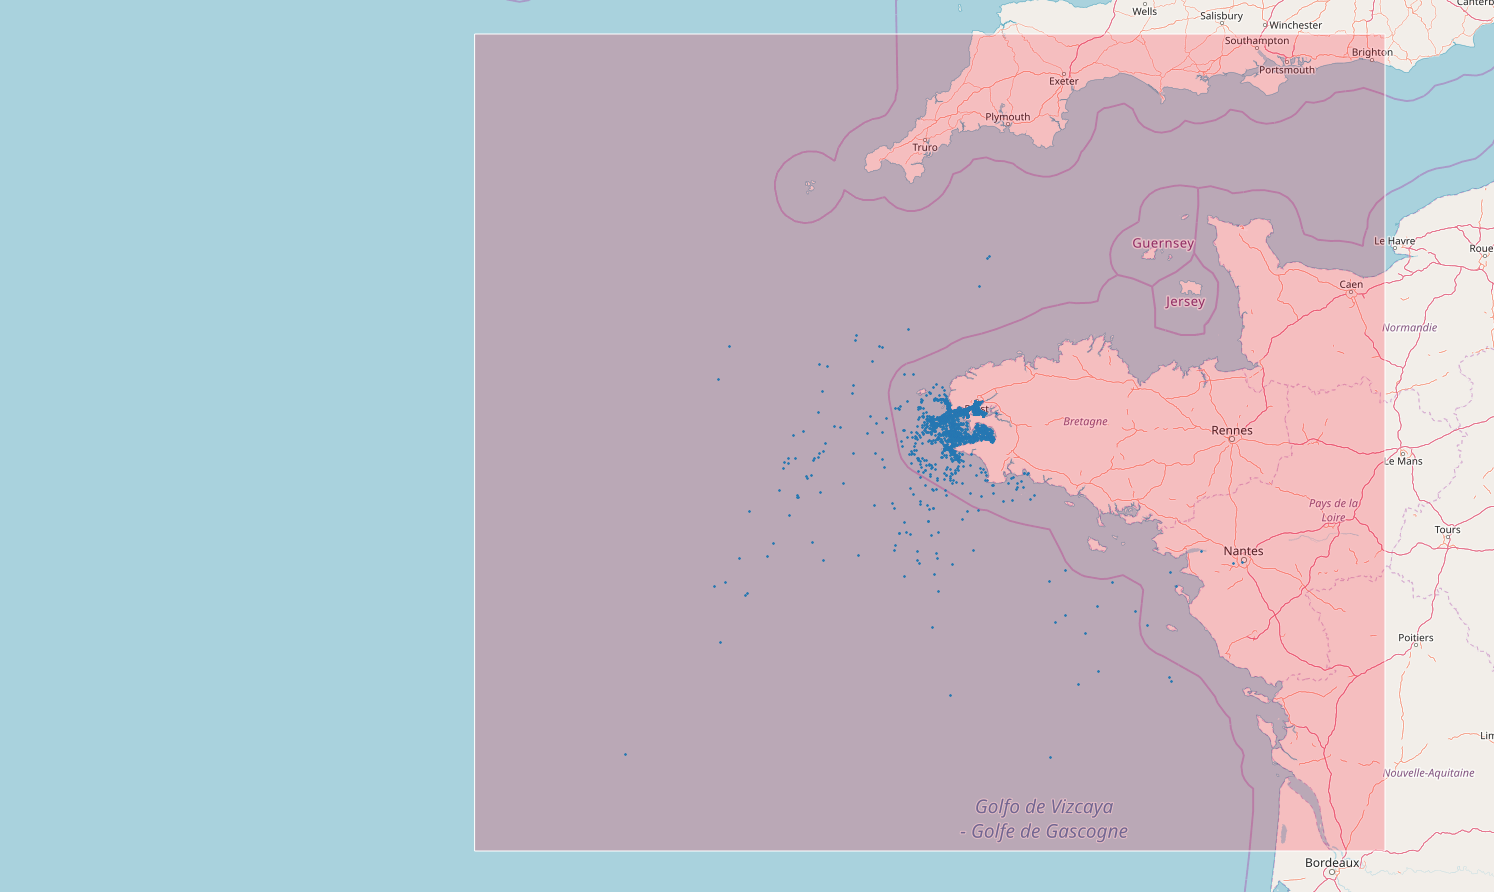
\includegraphics[width=\textwidth]{figures/Ch4/nari_DS_ex2.png}
\caption{Area of the Data-Set represented in the Red, with a sample of 50,000 AIS Positions.}
\label{fig:DS_Sample}
\end{figure}

Every AIS message provided in the dataset, is composed by the features that derive from the AIS dynamic information. In Table~\ref{Table: Data-Set Features}, we describe the dataset features by detailing their units and their unit range. 

\begin{table}[H]
\centering
\caption{AIS dynamic messages features description.}
\label{Table: Data-Set Features}
\begin{tabular}{@{}llll@{}}
\toprule
Feature & Description                  & Unit               & Range          \\ \midrule
MMSI    & Vessel Unique Identifier.     &                    & 0 to 99999     \\
Status  & AIS Navigational Status.     &                    & 0 to 15        \\
Turn    & Rate of turn, right or left. & degrees per minute & 0 to 720       \\
SOG     & Speed Over Ground.           & knots              & 0 to 111*      \\
COG     & Course Over Ground.          & degrees            & 0º to 360º     \\
X       & Longitude.                   & degrees            & -180º to +180º \\
Y       & Latitude.                    & degrees            & -90º to 90º    \\
Time    & Received Time-Stamp.         & Unix Time          &                \\ \bottomrule
\end{tabular}
\end{table}

The dataset not only contains the AIS dynamic information correspondent, but also, in separate files the related vessel static information of each vessel which has reported in dataset. By interpolating the MMSI reported in every AIS message, we were able to enrich each AIS dynamic message (or row of the dataset), with the static information related to the vessel which has produced the dynamic message. The vessel's static information contain information of the vessel's actual dimensions and type. The use of information related to the vessels characteristics is used in different types of behavioural analysis. In this work we used the vessel type as an key aggregation indicator, better described in Section~\ref{subsection: Vessel Type}.

\section{Data Ingestion}
\label{subsection: ch4 Data Ingestion}
Data Ingestion refers to the model, where the Data is input into the Framework. As mentioned in Chapter~\ref{chapter:Chapter 3}, for this work was assumed that the incoming data would be able to come in two different typologies, either from batches of AIS data or Live NMEA streams. 

Historical batches of AIS data (or datasets), are uploaded to this module via .csv files, which then are transformed into DataFrames using the Pandas\footnote{https://pandas.pydata.org}. For each imported batch of data, the features names must be pointed to the format we present in~\ref{subsection: Behavioural Point}
Although for the NMEA Streams the as the decoding of such streams was needed. The choice of methods to process and decode was not has trivial. As NMEA messages are received in high frequencies, the method to such streams into comprehensible AIS like data, needed to be stable and efficient. In order to achieve this, we used the python library libais\footnote{https://github.com/schwehr/libais}, which is implemented in the programming language C++, allowing a really efficient decoding of the incoming NMEA messages. 

In Chapter~\ref{chapter:Chapter 3}, we have identified two problems that occur when working with AIS real live. In order to mitigate the duplicated reception, each received messages is tagged with a unique identifier (UUID). For this present work, the created UUID will be done by considering the ID of the vessel(MMSI), and the time the received message was generated by the vessel. Thus, if two same UUID messages are received, we the second messages is discarded, and only the first received messages is considered.

The Framework was developed to be scalable, being able to handle different sources of AIS data, although for the purpose of this work, we limited the used Data to two main sources of Data. The Data-Set presented in Section~\ref{section: Data Analysis}, and the NMEA feeds made available by the Portuguese Navy.


\section{Data Pre-processing}
Data Pre-processing, represents the module that handles the raw/unprocessed AIS data, Cleaning, Transforms and Normalises every AIS messages, coming from the Data Ingestion Module. Every AIS message is transformed into our normalised representation of and AIS message, which we defined as a \textbf{Behavioural Point}, defined under in~\ref{subsection: Behavioural Point}.

\subsection{Latitude Longitude Normalisation}
In order to normalise the reported vessels positions, either from the AIS streams or the used Data-Set, we defined a set number of decimal cases used. This is done as most of AIS providers only assure a GPS precision of 0.0001 minutes accuracy, but what we found was that some reported positions come with up to 8 decimal cases, which can be caused just from how the Data-Set files were written.

So our normalisation process, was to assure that every vessel position was normalised to a precision on 4 decimal cases; as it represents a global position precision of 11m to 4m, as it is shown in Table~\ref{Table: Degree Precision}.

\begin{table}[H]
\centering
\caption{Degree precision versus the approximate radius of measured error.}
\label{Table: Degree Precision}
\begin{tabular}{lrrrr}
\hline
\multicolumn{1}{c}{\begin{tabular}[c]{@{}c@{}}Decimal \\ Places\end{tabular}} & \multicolumn{1}{c}{Degrees} & \multicolumn{1}{c}{\begin{tabular}[c]{@{}c@{}}Precision \\ Equator\end{tabular}} & \multicolumn{1}{c}{\begin{tabular}[c]{@{}c@{}}Precision \\ 45º N/S\end{tabular}} & \multicolumn{1}{c}{\begin{tabular}[c]{@{}c@{}}Precision \\ 67º N/S\end{tabular}} \\ \hline
0 & 1.0 & 111.3Km & 78.7Km & 43.5Km \\
1 & 0.1 & 11.3Km & 7.8Km & 4.4Km \\
2 & 0.01 & 1.13Km & 787.1m & 435m \\
3 & 0.001 & 111.3m & 78.7m & 43.5m \\
4 & 0.0001 & 11.3m & 7.8m & 4.4m \\
5 & 0.00001 & 1.3m & 0.7m & 0.4m \\ \hline
\end{tabular}
\end{table}
%\todo[inline]{Geohash - https://en.wikipedia.org/wiki/Geohash}

\subsection{Data Cleansing}
Data Cleaning refers to the process of cleaning the data which is wrongly defined or, has wrong types. When handling with sensor generated data is common that wrong sensor reading can occur. In AIS data, this errors tend to occur as AIS features that are not transmitted at all, or that are transmitted with values that don't correspond to the Feature value range. An example of this is having a Latitude being broadcast with values of 500.
Therefore, we discarded all AIS messages with reported features that were not inside the feature value range. The features value range considered for the proposed framework was the one presented in~\ref{Table: Data-Set Features}, which is the similar as the one presented by the authors in~\cite{Tu2016}, as the AIS default feature range.

\subsection{Behavioural Point}
\label{subsection: Behavioural Point}
Behavioural Point for this work, is our normalised feature representation of incoming vessel data. A $BP$ is a multidimensional point which is identified by the vessel id who produced the reported message. Therfore a $BP_{MMSI}$ can be represented as:

\[BP_{MMSI} = [t, x, y, SoG, CoG, NS]\]

Where the dimensions of the multidimensional $BP$ represents the features (Time, Longitude, Latitude, Speed Over Ground, Course Over Ground and Navigational Status) respectively.
Each $BP$ was correlated to one (one to one) identifier. The used identifier for this work was the Maritime Mobile Service Identity (MMSI). For this work the non replication of the MMSI by different vessel was assumed for work, this problem is discussed in Section\ref{subsection: Data Ingestion}.
Each $BP$, as described above is further enriched by extrapolating three additional features, making each $BP$ to be represented as:

\[BP_{MMSI} = [t, x, y, SoG, CoG, NS, VT, DtS, DtP, PN]\]

Where the additional features \emph{VT, DtS, DtP, PN} representing the vessel Type, Distance to Port, Distance to Shore, Port Name. These features are not reported from every AIS messages and need to be extrapolated afterwards. The methods used to extrapolated this features are presented under Section~\ref{section: 4 Feature Engineering}. 

\section{Feature Engineering}
\label{section: 4 Feature Engineering}

\subsection{Vessel Type}
\label{subsection: Vessel Type}
Vessel Type, is a classification system, where each vessel is categorised by the type of activities it preforms. Classified by a numeric scale from 0 to 99. The first digit represents the general activity category of the vessel, and the combination of the first digit with the second represent the specific activity of the vessel. In Table~\ref{Table: Vessel Type Description} we list all the general vessel categories which are associated with the first digit of the vessel type feature, but also we present the specific vessel categories for the more frequent vessel types occurring on the dataset.

\begin{table}[H]
\centering
\caption{Vessel Type categorisation and most frequent representation.}
\label{Table: Vessel Type Description}
\begin{tabular}{@{}clll@{}}
\toprule
First Digit & General Category                                        & Relevant Categories                                        &                                                                                         \\ \midrule
1           & Reserved                                                &                                                            &                                                                                         \\
2           & Wing In Ground                                          &                                                            &                                                                                         \\
3           & Special Category                                        & 30 - Fishing                                               & 30 - 286(6\%)                                                                           \\
4           & High-Speed Craft                                        &                                                            &                                                                                         \\
5           & Special Category                                        &                                                            &                                                                                         \\
6           & Passenger                                               &                                                            &                                                                                         \\
7           & \begin{tabular}[c]{@{}l@{}}Cargo\\  \\  \end{tabular} & \begin{tabular}[c]{@{}l@{}}70 - Cargo\\ \\ \end{tabular} & \begin{tabular}[c]{@{}l@{}}70 - 1,511(33\%)\\ 79 - 273(6\%)\\ 71 - 217(5\%)\end{tabular} \\
8           & Tanker                                                  & 80 - Tanker                                                & 80 - 342(7\%)                                                                           \\
9           & Other                                                   &                                                            & 99 - 1,192(26\%)                                                                         \\ \bottomrule
\end{tabular}
\end{table}

For the used Data-Set described above in Section~\ref{section: Data Analysis}, the Static Vessel Information is available for all the vessel in the Data-Set. Although, when handling Real-Time NMEA streams or other Batches of Data, the Vessel Static information is not available or broadcast. This, creates a problem of not having the Vessel Type information which is used to query our Trajectory Data-Base.
For this we developed a \textbf{Web Scrapping application}, described in the following subsection.

\subsubsection{Vessel Type Scrapper}
Web Scrapping is used to extract information from freely available websites. For the sole purpose of this work, we developed an application that would retrieve the Vessel Type information from a "well known vessel traffic webpage".
By providing the vessel MMSI to the Vessel Type Scrapper, we retrieve the html webpage data that contains all the static vessel information available on the "well known vessel traffic webpage". From the html data we, striping the html tags, and the non relevant specific webpage information, we access Vessel Type, as it is presented in Figure~\ref{fig:Scraper}.

\begin{figure}[H]
\centering
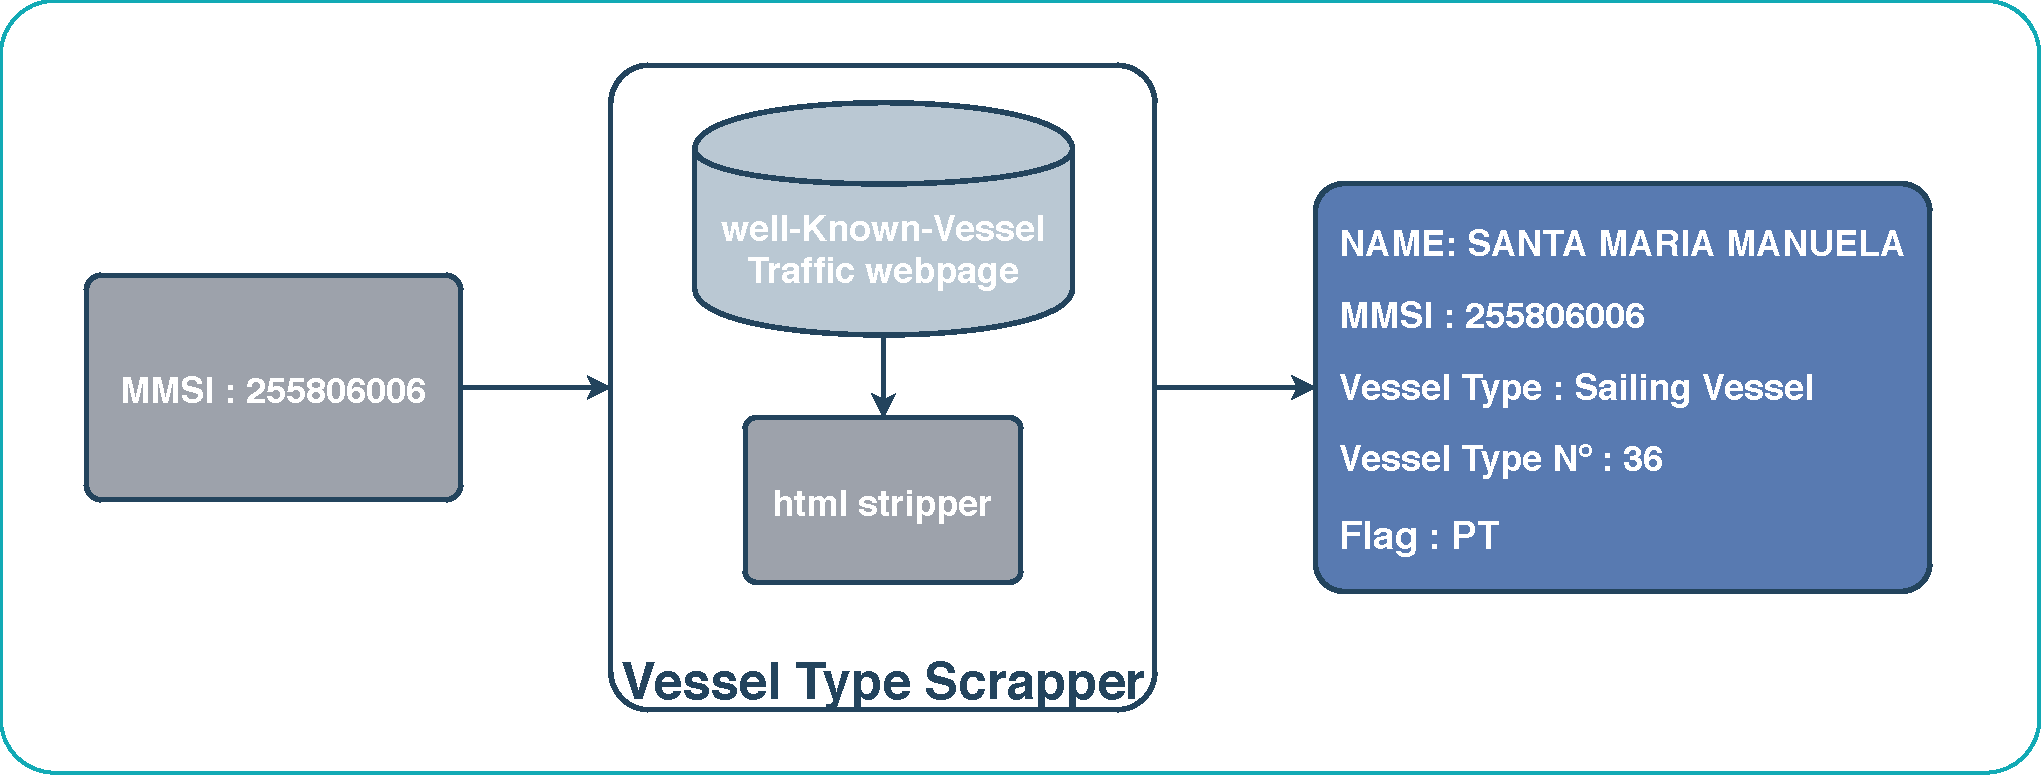
\includegraphics[width=\textwidth]{figures/Ch4/scrapper}
\caption{Example of the Vessel Type Scrapper retrieved information for Vessel MMSI: 255806006}
\label{fig:Scraper}
\end{figure}


\subsection{Distance to Coast}
\label{subsection: Distance to Coast}
Distance to Shore influences, the navigational behaviour for the major part of Vessel Types. In order to enrich the $BPs$ which will feed the Anomaly Detection modules, and as the distance to shore is without a doubt a valuable aggregation feature for the maritime domain. We extrapolated the Distance to Shore for every received AIS message. 

Although in order to calculate the distance to shore effectively either over historical batches of data or in real time to streams of AIS data, a efficient representation of the coastline is needed. 
For this we used the ocean coastline data\footnote{http://naturalearthdata.com}. This representation has mapped Global coastline in a vector of \textbf{547,503} points, which is equivalent having a 1:10m Global coastline representation.

The calculation of the closest point was done with a Nearest Neighbour approach, using the Ball Tree algorithm. The choice of this algorithm was done, due to the high volume of data we were using, and the possibility of using the Haversine Distance measures in the already implemented methods from \footnote{http://scikit-learn.org/stable/modules/generated/sklearn.neighbors.BallTree.html}.

Haversine is the most commonly used distance metric in the vessel navigation. As both Latitude(y) and Longitude(x) features are represented in a spherical coordinate system, the use of the most common Euclidean distance is not applicable. Thus we used the Haversine Equation~\ref{eq: Haversine}, represented under.

\begin{equation}
d = 2r sin ^{-1} \sqrt{sin^2(\frac{lat_{p_2}-lat_{p_1}}{2})+cos(lat_{p_1})cos(lat_{p_2})sin^2(\frac{lon_{p_2}-lon_{p_1}}{2})}
\label{eq: Haversine}
\end{equation}

Where $d$ takes as input $({p_1}, {p_2})$, and it calculates the haversine the 2 point represented as $p1(lat_1, lon_1)$ and $p2(lat_2, lon_2)$. $r$ represents the approximate radius of the Earth which for this work we considered \textbf{6,367Km}.

\subsubsection{Distance to Port}
Distance to Port, to the maritime scenario, and more specifically maritime international trade, represents an additional feature which is of great importance. The Estimation of Time of Arrival presents itself as a necessity for container terminals, as this terminals base operational decisions on such estimation. The estimation of time of arrival, and the prediction of the arrival port based on past vessel trajectory information, are two tasks which use the distance to port feature for such purpose, \cite{Moussa2018ScalableSpark}, \cite{Rosca2018PredictingRoutes}.

This being said, we enriched each $Behaviour Point$ by calculating the actual nearest port, and the distance to it. To achieve this, we used a similar approach as explained above in Subsection~\ref{subsection: Distance to Coast}.

Although, getting a list of every port was not trivial, as there are numerous ports around the World, and such information is not 
centralised nor normalised.
We accessed the detailed information of the World Port Indexes in \footnote{http://msi.nga.mil/MSISiteContent/StaticFiles/NAV\char`_PUBS/WPI}. The World Port Index data was in a GIS(Geographic Information System) shapefile format, which is common format for the Maritime Domain, but not usable in our Framework. Therefore, we firstly normalised the data format using the Python dbfread\footnote{http://dbfread.readthedocs.io}, and then stored the normalised port data in our data-base. 
For each of the \textbf{3,865} ports we extracted the respective Port position, Country, and Name. 
In Figure~\ref{fig: 4 Ports} we present the port position over the Iberian coast in Orange.

\begin{figure}[H]
\centering
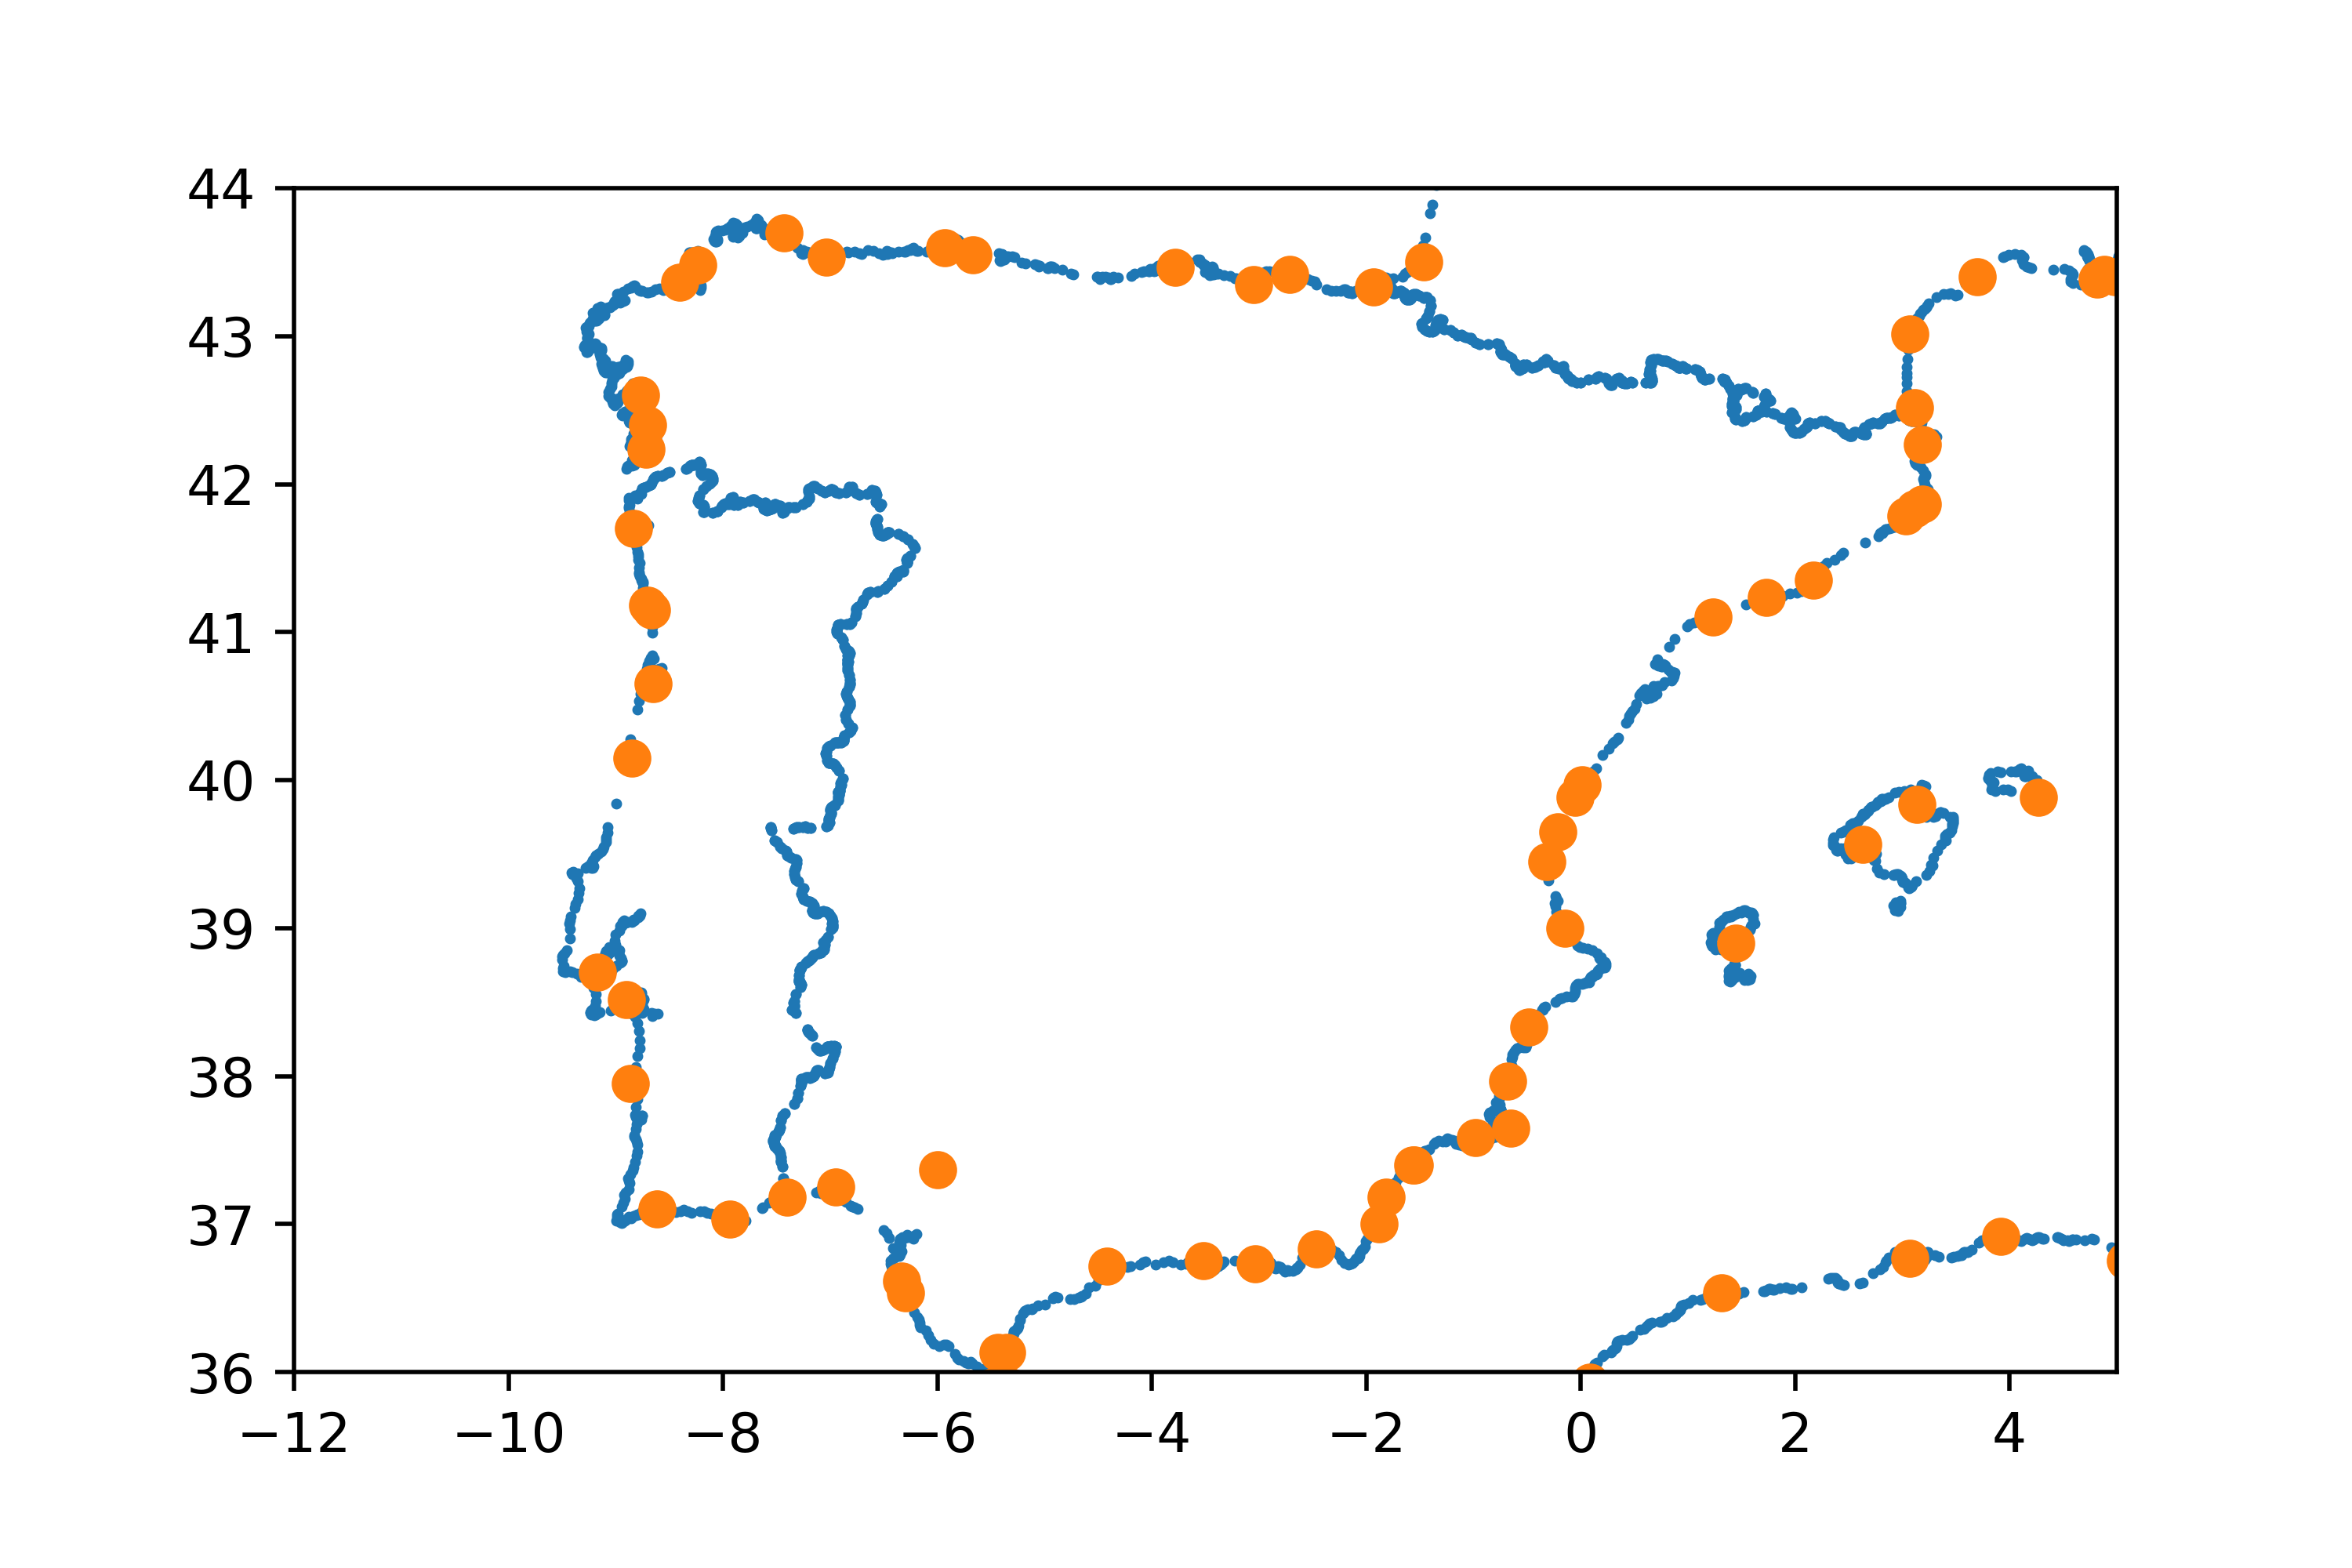
\includegraphics[scale = .9]{figures/Ch4/ports.png}
\caption{Iberian Ports(in orange), with the considered coastal Points(in Blue)}
\label{fig: 4 Ports}
\end{figure}

\subsection{Stopped/Moving}
\label{subsection: Stopped/Moving}
Enriching the reported $BPs$ by determining if at this point in time a vessel was in fact moving or stopped represents an overall information gain over the whole vessel trajectory. Such information can be used for the understanding of the normal vessels behaviour, or the detection of global points of interest.
Thus, in order to gain such information, we used two different method. The first one was a point based approach, where we infer if whether a vessel is stopped or moving based on the last report, this method is described under in this Subsection. The second approach involves the use of a vessels past trajectory information, we present this approach further in this Chapter in Section~\ref{subsection: Smoothed Stopped / Moving}.

\textbf{Rule Based Approach}:
This approach is vastly used in the literature, as it is the simplest way to characterise the stopping of a vessel, based solely on the vessels reported speed or as reported by the AIS the Speed Over Ground (SOG). Thus, a $BP$ which has a reported speed under a certain defined threshold $\Delta$ is considered as stopped and the opposite are considered moving. As it is shown in equation~\ref{eq: MovingRule}, where $BP_n$ represents actual Behavioural Point we want extrapolate the stopped or moving feature.

\begin{equation}
kinematic status(p_n) = \left\{\begin{matrix}
BP_n.SOG > \Delta; & Moving\\ 
BP_n.SOG \leq  \Delta; & Stopped
\end{matrix}\right.
\label{eq: MovingRule}
\end{equation}

The most commonly used $\Delta$ value found in literature was 0.5 knots.
This approach despite fitting most of the vessels behaviours, for the some types of fishing vessels it does not fit such behaviours. This occurs as some fishing activities, require the vessel to be drastically slow down for short periods of time.
In Figure~\ref{fig: 228858000}, we present a fishing vessel trajectory, where points represented in blue are considered as stopped points.   

\begin{figure}[H]
\centering
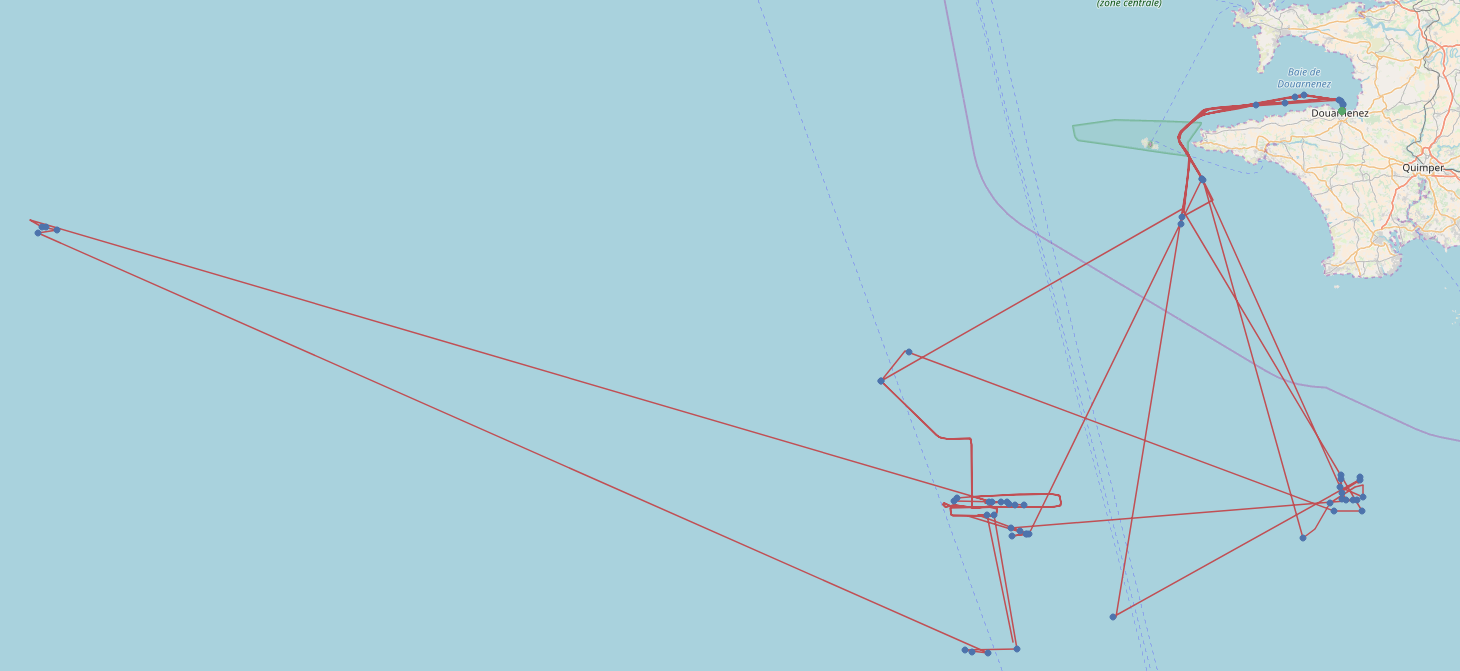
\includegraphics[width=\textwidth]{figures/Ch4/simplestopMoving228858000_cropped.png}
\caption{Fishing vessel (MMSI: 228858000) trajectory. Where the Blue points represent the Stoped points on the overall trajectory.}
\label{fig: 228858000}
\end{figure}

\section{Unsupervised Trajectory Extraction}
\label{section: 4 Unsupervised Trajectory Extraction}
In this Section we present our interpretation and the definition of what was for this work considered as a vessel trajectory. 

\subsection{Trajectory Definition}
\label{subsection: Trajectory Definition}
Representing a trajectory in a optimal way, can become a difficulty task in the maritime domain. Currently there are a vast number of solutions described in the literature. They, represent a trajectory differently, depending on the type of problem.

Our approach to represent a maritime trajectory, was to consider a trajectory as a whole. This is, as vessel are obliged to broadcast their AIS information in a semi-continuous rates. By normalising each broadcast by defining a \textbf{Behavioural Point}, we can aggregate each $BP$ based on the $BPs$ vessel identifier which is the vessel MMSI. Thus the aggregation of $BPs_{MMSI}$ represents for us a trajectory, which can be represented as:
\[TR_{MMSI} = BP_{MMSI_1}, BP_{MMSI_2}, BP_{MMSI_3}, BP_{MMSI_4}, \cdots , BP_{MMSI_n}\]
Every trajectory is then sorted, and kept sorted based on the Time-Stamp of each $BP_{MMSI}$. The representation of the $BPs$ over a time allows us to consider a each trajectory ($TR_{MMSI}$) as a multivariate time-series.
Each trajectory, can be then defined as a group of $N$ time-series. Where $N$ represents the number of features considered for the $BPs$ definition.

Nevertheless, what was considered as most relevant, for our definition of a trajectory was the effectiveness, and scalability of such representation. This is, the effective adding of new $BPs$ to a trajectory, and the accessing of historical trajectories in effective time. We achieved this by implementing the data-base in Cassandra. From such we defined a set of pre-defined queries to which allowed the effective access to a whole or partial trajectory, in near real time.
In Figure~\ref{fig: TrajectorySMM_example} we represent an example of the vessel trajectory which was plotted over a map. 

\begin{figure}[H]
\centering
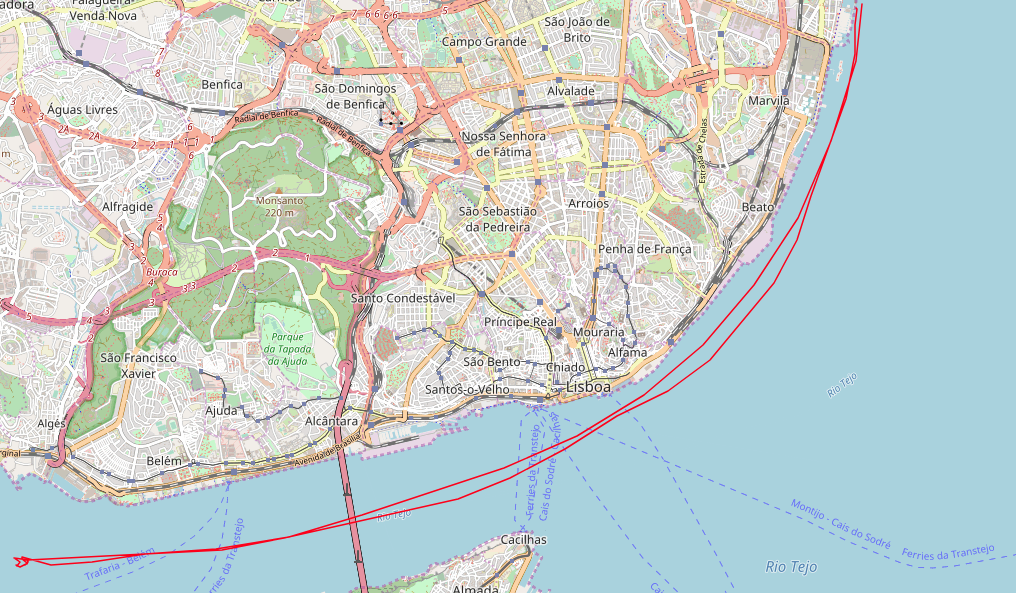
\includegraphics[width=\textwidth]{figures/Ch3/traj_example.png}
\caption{Trajectory snapshot(2017-11-05 10:22 to 2017-11-05 22:42) from Vessel MMSI: 255806006}
\label{fig: TrajectorySMM_example}
\end{figure}

The same trajectory plotted above, is also represented as a multivariate time-series, in Figure~\ref{fig: MTimeSeries_example}, by just considering the four most relevant kinematic features of a $BP$, the positional features (where $x$ represents the Longitude, and $y$ represents the Latitude) and the speed and course features. 


\begin{figure}[H]
\centering
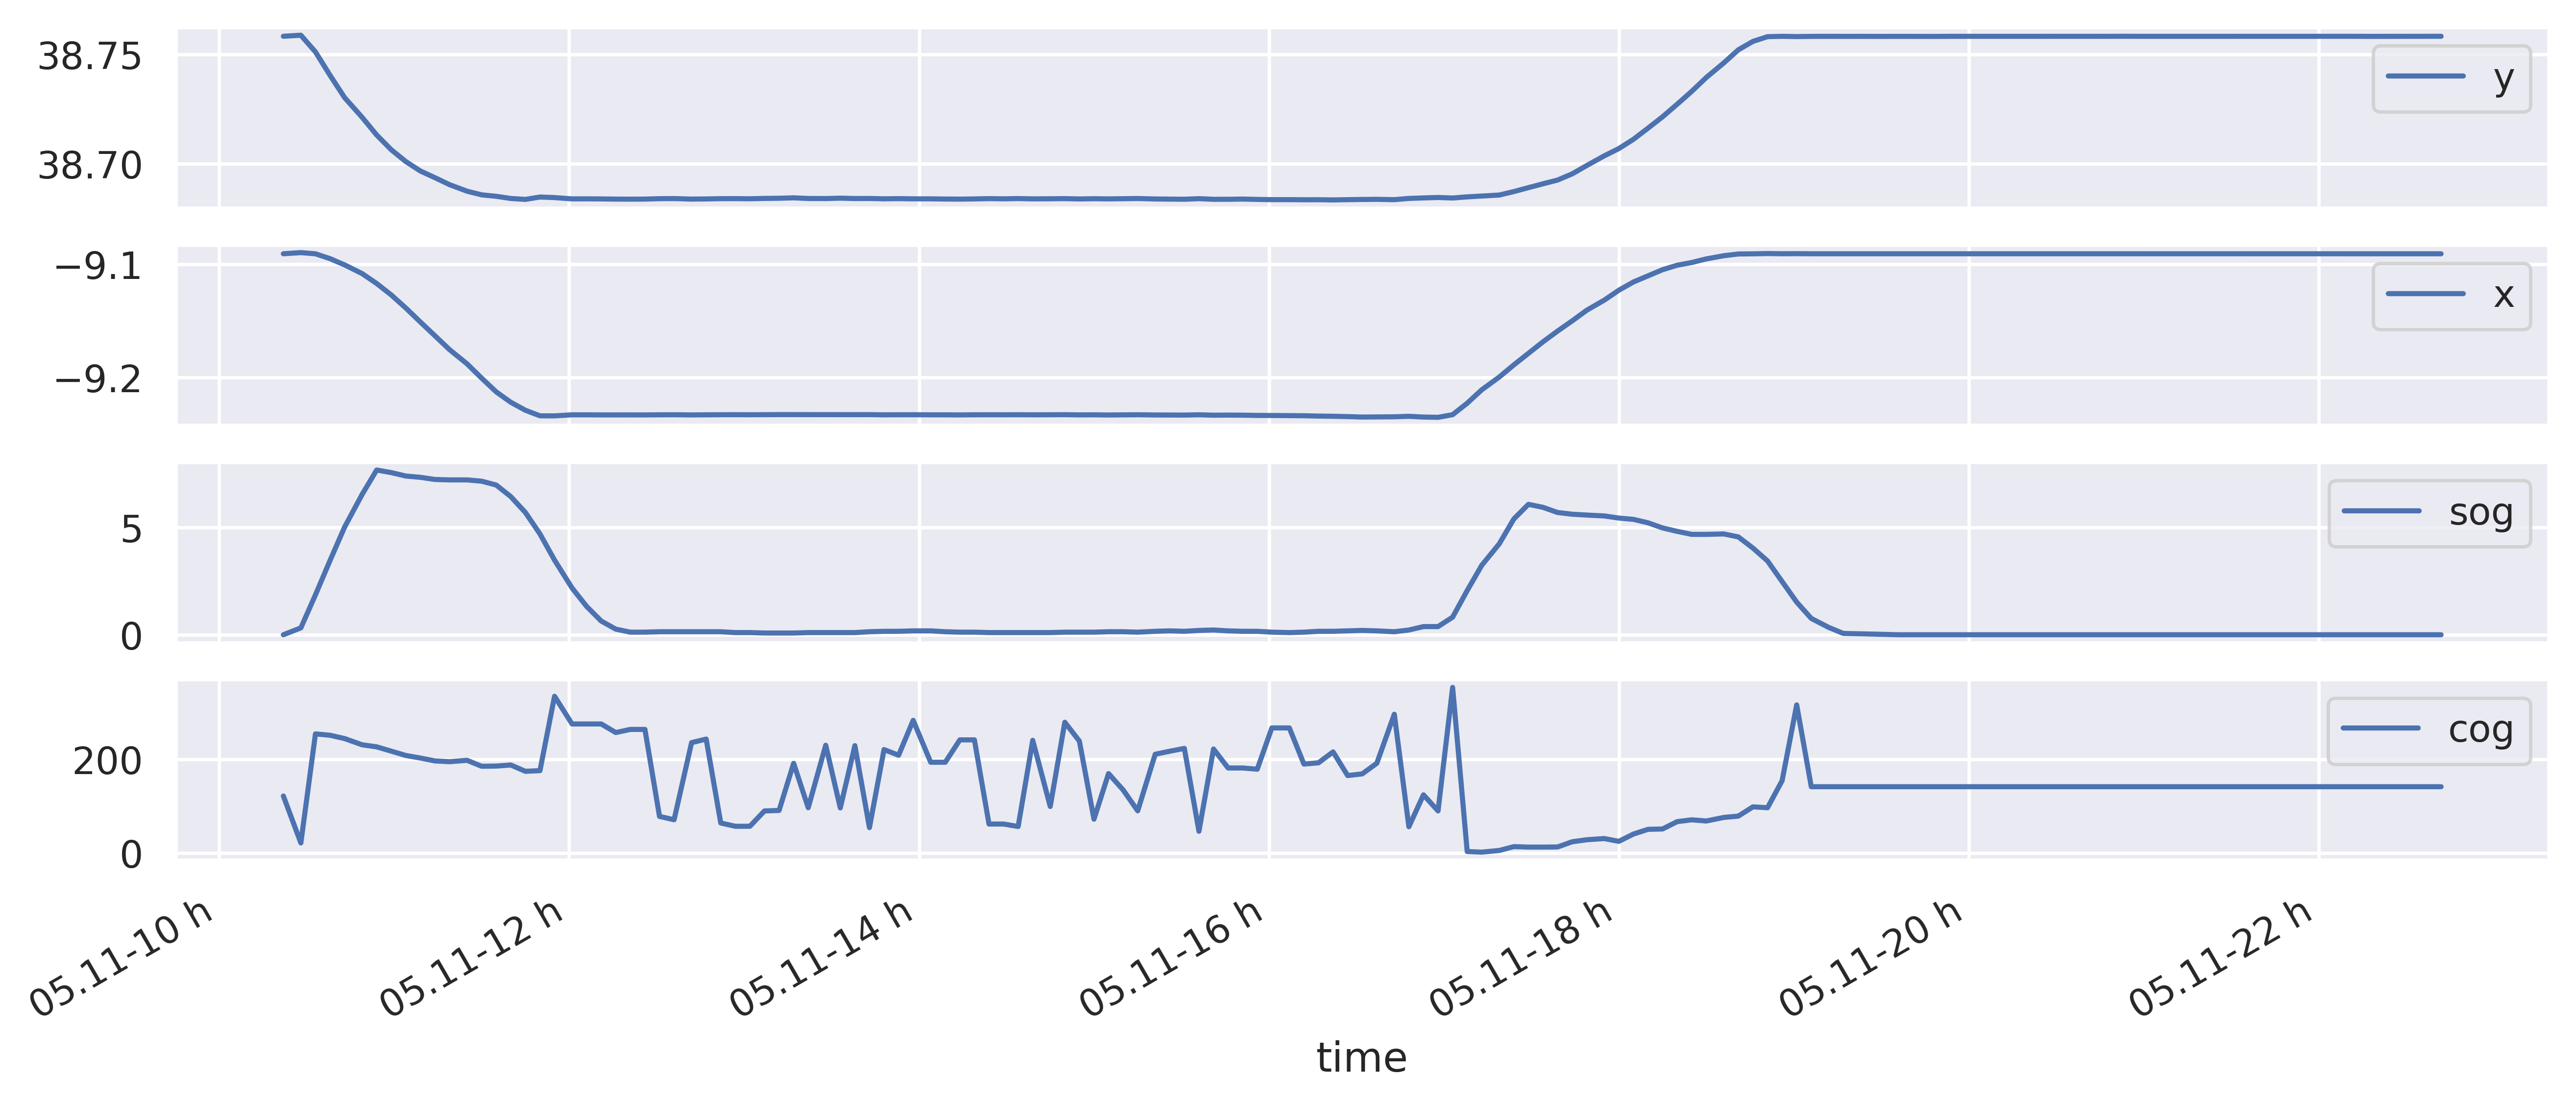
\includegraphics[width=\textwidth]{figures/Ch3/ts_example.png}
\caption{Trajectory represented in Figure~\ref{fig: TrajectorySMM_example}, presented as a multivariate time-series.}
\label{fig: MTimeSeries_example}
\end{figure}

\subsection{Smoothed Stopped / Moving}
\label{subsection: Smoothed Stopped / Moving}
In order to resolve the problem presented in Section~\ref{subsection: Stopped/Moving}, where the rule based stopped/moving approach had problems when dealing with some type of fishing activity trajectories. 
And also as a trajectory could be overseen as a multivariate time-series. We used a commonly used time-series analysis technique, \emph{Rolling Mean}. 
By smoothing the vessels $SoG$ time-series, based on the previous configurable $W$ $BPs$, where $W$ represent the window size considered. We smooth the random or abrupt variations in the observed speed features, which will in the end better describe the kinematic movement behaviour presented by these fishing vessels. 
The configurable $W$, allows the end-used of this framework, to configure the smoothness of the over the reported speed feature. This ultimately leads to a better representation of the vessel kinematics, which will be used for the anomaly detection methods presented in Subsection~\ref{subsection: 4 Time-Space Incompatibility},~\ref{subsection: 4 Navigational Status Validation} and~\ref{subsection: 4 Vessel Rendezvous}.

\begin{figure}[H]
\centering
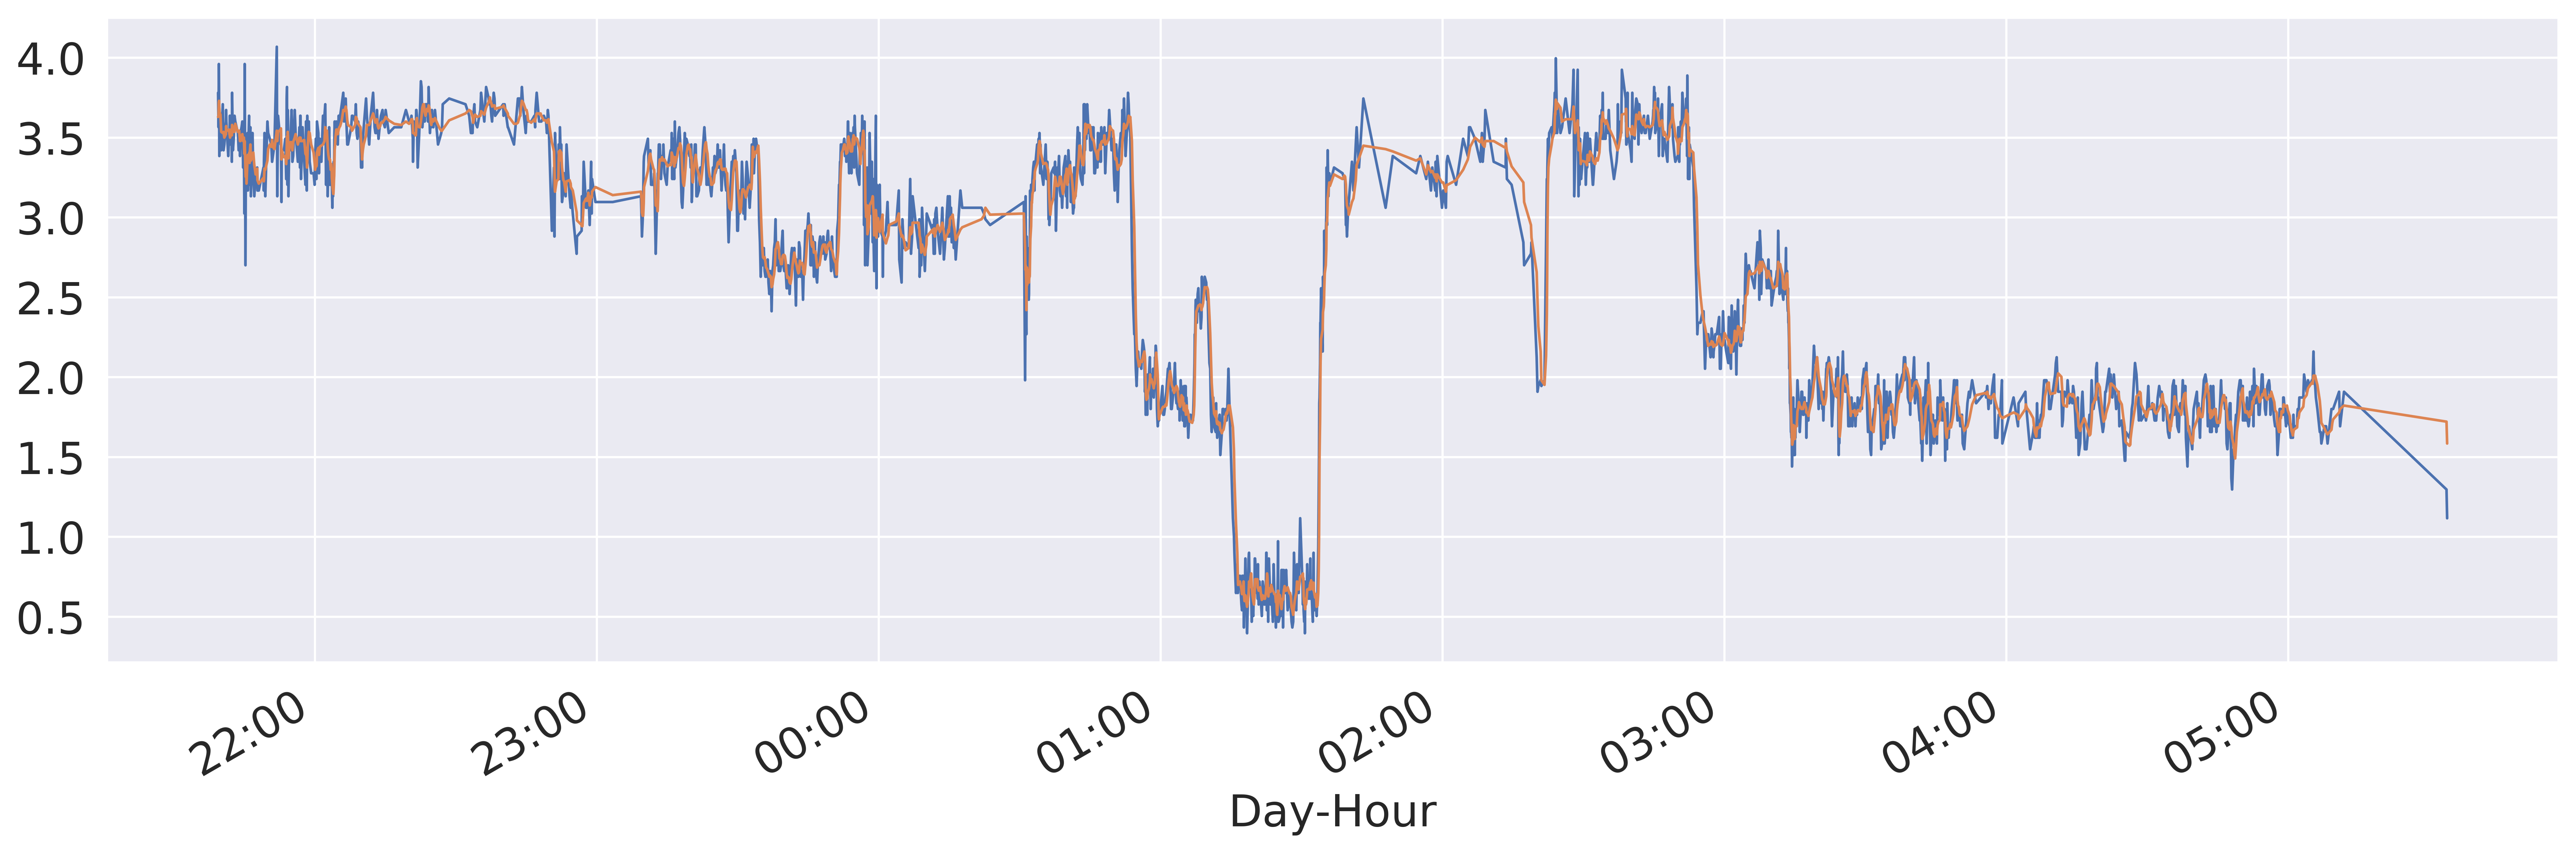
\includegraphics[width=\textwidth]{figures/Ch3/ts_smoothed.png}
\caption{Snapshot of Trajectory represented in Figure~\ref{fig: 228858000} SOG feature presented as a time-series.}
\label{fig: 228858000 ts smoothed}
\end{figure}

\section{Anomaly Detection Service}
\subsection{Time-Space Incompatibility}
\label{subsection: 4 Time-Space Incompatibility}
Time Space incompatible corresponds to an anomalous or incoherent situation where the reported actual vessels position is not compatible if compared with previous reported positions, and vessels kinematics. The detection of this situation, is also represented as an Anomaly Requirement \emph{$AR_4$}, in Section~\ref{section: Framework Requirements}.

In order to detect this incoherence's, we developed a method that takes as input an historical vessels trajectory $TR_{MMSI}$, and for each Behavioural Point ${BP_{MMSI}}^{T-1}$ we estimate the vessels position at instance ${BP_{MMSI}}^{T}$.
The estimation is done by assuming that a vessels movement can be represented in a \emph{Linear Motion}. As vessels tend to move in the most economical way, the Vessels travelled distance, was calculated, using the formula:
\begin{equation}
Distance = Velocity \cdot \Delta Time
\label{eq: dvt}
\end{equation}
Where $\Delta Time$ represents the actual time shift from point $(T-1)$ to $(T)$. The $Velocity$ represents the $BP_{SOG}$ feature, which is reported in knots. The $Velocity$ is firstly converted to $m/s$By calculating the Equation~\ref{eq: dvt} for each $BP^{T}$ based on the reported Position of the previous $BP^{T-1}$, and assuming a vessel tend to move in a somewhat linear motion, we can predict that vessel should be in a distance radius of $D$ for the next $BP^T$, as it is shown in Figure~\ref{fig: dvt}.

\begin{figure}[H]
\centering
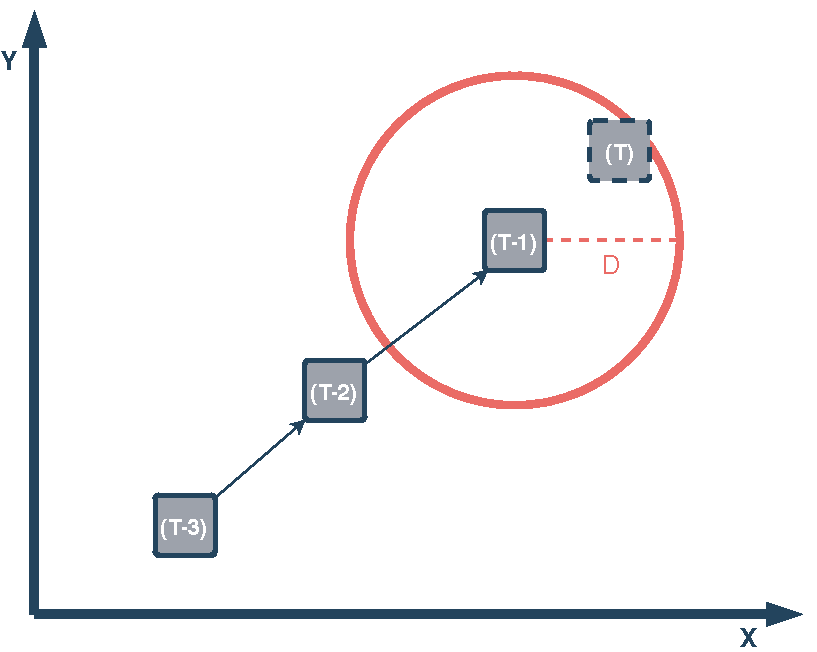
\includegraphics[scale = .6]{figures/Ch4/DVT.pdf}
\caption{Linear estimation based on the previous reported $BP$.}
\label{fig: dvt}
\end{figure}

By defining a configurable \emph{Distance Factor Threshold} $dft$, representing a factor that would be multiplied by $D$, is possible to deduct that, if the a vessel at Time $BP^{T}$ is at a distance superior than $(D.dft)$, it is considered at a incoherent position. Therefore it is reported as anomalous.

The emphasis of this Section was on the detection of Time-Space Incompatibly, which is depend on the level of error acceptance is achieved using the methods above. 
Although by assuming that vessels have a huge inertia, making them unable to perform quick changes of speed and direction, the authors in \cite{Sadowski2015AlgorithmsCompression} present a \emph{Linear Estimation Algorithm}.
As the reported $CoG$ represents the direction of movement, it is possible to based on Equation~\ref{eq: dvt}, to estimating the position of the Vessel, opposed to the distance from previous position. This is done by firstly calculating the Latitude and Longitude \emph{shift} based on the $BP^{T-1}$, using Equation~\ref{eq: dvt_xy}.

\begin{equation}
\begin{matrix}
\Delta X = Distance \cdot sin(COG \cdot \pi/180)
\\
\Delta Y = Distance \cdot cos(COG \cdot \pi/180)
\end{matrix} 
\label{eq: dvt_xy}
\end{equation}
Where $\Delta X$ and $\Delta Y$  represent the Longitude and Latitude features shift respectively. $Distance$ represents the Distance which is calculated using the Equation~\ref{eq: dvt}. Finally, the estimated coordinates of the vessel are: 
\begin{equation}
\begin{matrix}
X' = X + \Delta X 
\\ 
Y' = Y + \Delta Y
\end{matrix} 
\label{eq: estimated_dvt_xy}
\end{equation}



\subsection{Navigational Status Validation}
\label{subsection: 4 Navigational Status Validation}
AIS Navigational Status describes the vessel current activity based on a set static set of defined status, as shown in Table~\ref{Table: AIS Status}.

\begin{table}[H]
\centering
\caption{AIS Navigational Status enumeration.}
\label{Table: AIS Status}
\begin{tabular}{@{}cl@{}}
\toprule
\begin{tabular}[c]{@{}c@{}}Navigational \\ Status Value\end{tabular} & \multicolumn{1}{c}{Description} \\ \midrule
0 & under way using engine \\
1 & at anchor \\
2 & not under command \\
3 & restricted manoeuvrability \\
4 & constrained by draught \\
5 & moored \\
6 & aground \\
7 & engaged in fishing \\
8 & under way sailing \\
9 - 14 & reserved for future use \\
15 & Default \\ \bottomrule
\end{tabular}
\end{table}

The Navigational Status requires to be manually set, and constantly updated (according to the current vessel activity), by the vessel crew members.
This creates the problem of relying on Human action to update the actual vessel navigational status, which is prone to errors. 
The use of the wrong navigational status being considered an Anomaly represented as $(AR_4)$ in Section~\ref{section: Framework Requirements}, our approach towards the detection of such Anomaly, started by firstly gaining insight of each navigational status, and their usage at seas.
By accessing maritime knowledge via Maritime Officers, we enriched our previous description of each navigational status, by classifying the appropriate \emph{Stopped or Moving Label} to each status. Maritime Officers based the expected kinematics of each navigational status provided the following Table~\ref{Table: AIS Status Moving or Stopped}.
\begin{table}[H]
\centering
\caption{Expert stopped or moving label over the AIS navigational status.}
\label{Table: AIS Status Moving or Stopped}
\begin{tabular}{lc}
\hline
Expert Label     & Navigational Status Number \\ \hline
Stopped          & 1, 5, 6                    \\
Moving           & 0, 7*, 8                   \\
Non-Quantifiable & 2, 3, 4, 15                \\ \hline
\end{tabular}
\end{table}
$7^*$ (Engaged at Fishing) represents a special navigational status which cannot be validated with a stopped or moving analysis. Our efforts to validate this specific status are presented under in Subsection~\ref{subsection: Fishing Activity Detection}.

The actual navigational status validation, is done as a \emph{point based comparison}. By comparing the previous $BPs$ enriched feature \emph{Smoothed Stopped or Moving}(Section~\ref{subsection: Smoothed Stopped / Moving}) with the stopped/moving label Maritime Experts has defined for each Navigational Status.
An example for this validation could be:
If a $BP$ has been received with the Navigational Status \textit{0 - under way using engine}, but the reported Kinematics describe it as \textit{Stopped}, which for this Status should be \textit{Moving}.

\subsection{Fishing Activity Detection}
\label{subsection: Fishing Activity Detection}

Based on the Navigational Status Validation presented above we decided to enrich this methods with the detection of a special navigational status, the fishing activity (Navigational Status - 7 - Engaged in Fishing). 

Fishing is a activity that generates huge profits for the global maritime lobby. This activity being so profitable and competitive between fishing companies, generates a problem for the Maritime Authorities. To avoid informing other fishing vessel of lucrative "fishing spots", fishing vessels try to hide their location as most as possible. This behaviour is anomalous when AIS is turned off. Fishing vessels are more prone to undermine the fishing competition, leading to Illegal Unreported and Unregulated fishing \footnote{http://fao.org/iuu-fishing/en/}(IUU).  Linked to IUU is the depletion of fish stocks, as well as the destruction of marine habitats and therefore putting honest fishers at an unfair disadvantage and thus weakening coastal communities, particularly in underdeveloped countries~\cite{kroodsma2018TrackingFisheries}.

A vessel fishing activity is commonly defined as the period of time by which a vessel has fishing gear in the water. Since at the time we didn't have access to any Maritime Expert Classified datasets, we focused on the validation of this particularly navigational status (7 - engaged in fishing) by analysing the kinematic features capable of inferring whether the vessel is currently fishing or not. 
The main characteristic that identifies the fishing activity is the fast variation of direction together with a change in the speed. This can be seen as a generalisation as there are multiple different fishing, each different one having its own specific kinematic behaviour.
Nevertheless, we claim that a fishing behaviour may be reasonably assumed to be highly dependent on speed variations. Specifically speed variations allow the fishing activity to be described by two main behavioural patterns. The first one is the \emph{high speed behaviour}, typical of a vessel steaming at normal cruising speed from a fishing spot to another. The other one, the \emph{low speed behaviour} is represented by the speed when vessels tend to drop the fishing gear in the water, or preform other manoeuvres which can be related to the fishing activity itself. Based on the work presented by the authors in ~\cite{DeSouza2016ImprovingLearning, Natale2015MappingData, Mazzarella2014DiscoveringFootprints}, this double speed behavioural profile may be represented as a bi-modal distribution of speeds. Assuming that the speed profiles are characterised by only two speed modes, it is reasonable to apply Expectation Maximisation Gaussian Mix Models in order to estimate two distribution parameters, namely the respective mean and standard deviation of each mode, and to assign the observations to one of these behavioural profiles.
Such bi-modal Gaussian distributions may be appreciated in Figure~\ref{fig: 4 gmm_example}, where a typical histogram of the distribution of the reported speed is plotted.


\begin{figure}[H]
\centering
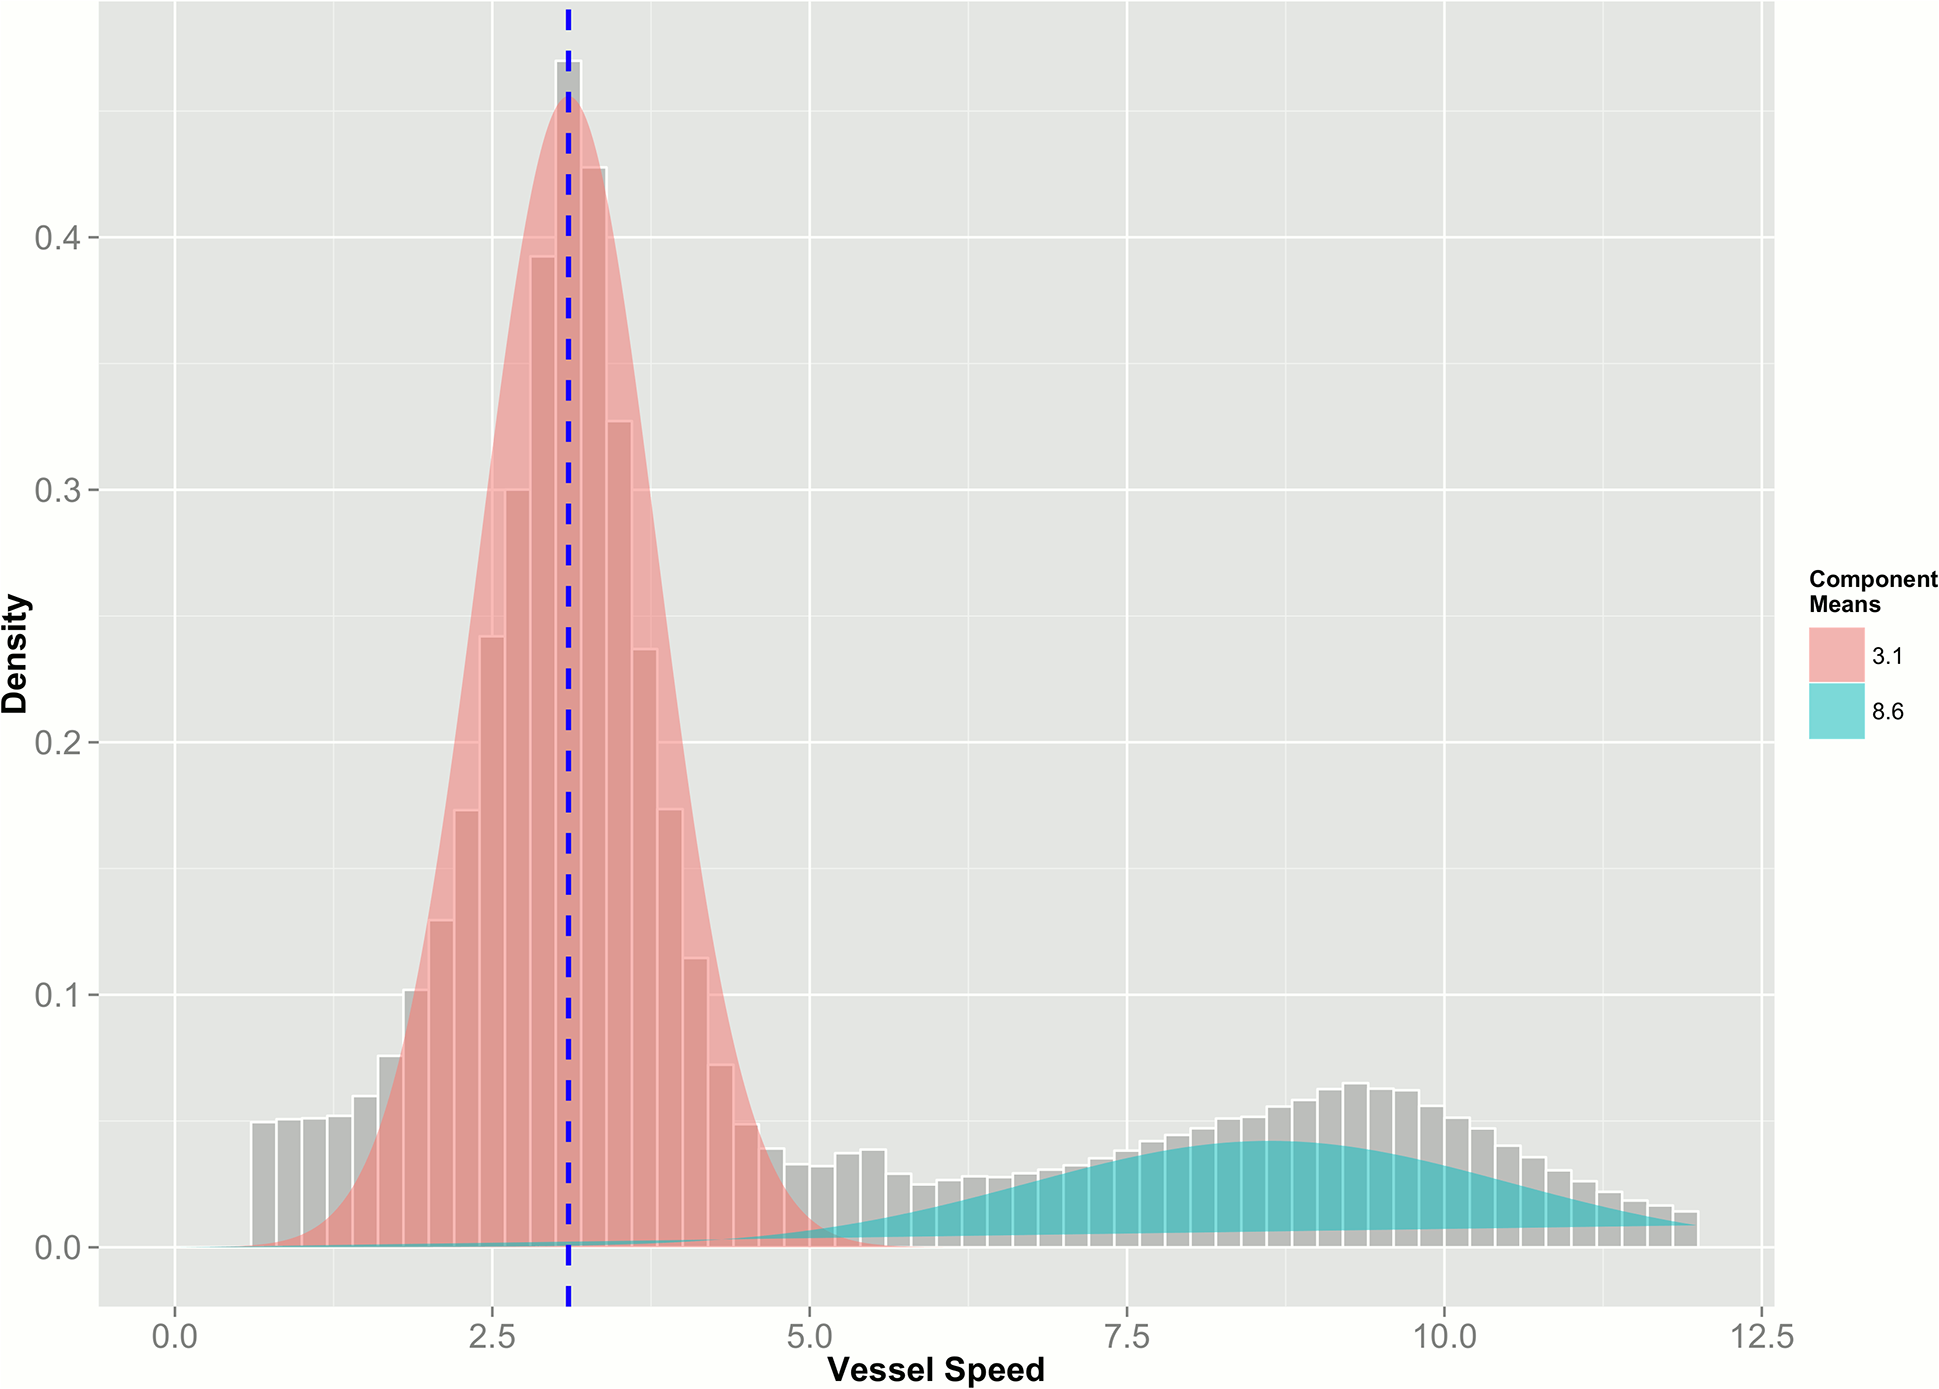
\includegraphics[scale = .7]{figures/Ch4/gmm_example.png}
\caption{Example of speed profile for one vessel fitted for a bi-modal distribution. Reprinted from~\cite{Natale2015MappingData}.}
\label{fig: 4 gmm_example}
\end{figure}

 
From the presented dataset in Section~\ref{section: Data Analysis} we fitted a Gaussian mix model to our data. This was done based on the approach presented by the authors in~\cite{Natale2015MappingData},  where we used the already developed methods of~\footnote{http://scikit-learn.org/stable/modules/mixture.html}. From the already  processed dataset, we filtered only the $BPs$ that were type Fishing Vessels (Vessel Type 30). This reduced the number of considered $BPs$ to approximately 3 Million. To avoid irregular vessel movement, and analyse the vessel movement patterns that could induce the vessel fishing activity, we filtered the $BPs$ that would be a distance of more than 2 Nautical Mile from shore, leading to a sub dataset of $436,043$ possible Fishing $BPs$.
The results and the discussion from the usage of this module are presented in Subsection~\ref{subsection: ch5 fishing validation}.

\subsection{Vessel Rendezvous}
\label{subsection: 4 Vessel Rendezvous}
Another anomaly requirement~\emph{AR6} which was defined by the \textsc{Marisa} project, was the development of services, able to detect when two or more vessels are approaching close to each other. The detection of this anomaly is complex, as it can occur in multiple scenarios. Although, for this current work we focused on the detection rendezvous, from huge batches of historical data, in a effective way. 

Rendezvous occurs when two vessels meet allowing for the transfer of cargo, fuel, provisions, fish catch, crew or gear from one vessel to another. When transshipping takes place far from port, it can allow fishing vessels to avoid scrutiny at port and conceal suspicious activities like illegal fishing. But most alarming this practice leads to other nefarious activity, ranging from smuggling to human trafficking,~\cite{Miller2018IdentifyingBehavior}.

Nevertheless, the concept of rendezvous is still quite complex to formalise by maritime officers, as there numerous legislation. Thus, for the purpose of this work, and because the emphasis is on the detection of possible rendezvous, a simplification of this vessel interaction is assumed, therefore: 

~\emph{Vessel Rendezvous}, is then defined for this work as, the interception or closeness of two or more vessels, in a configurable time period.

%by defining a distance threshold~\textbf{d}

In order to detect the rendezvous occurrences from multiple vessels, each single trajectory is partitioned into~\textbf{t} time-groups e.g. a time-group of 5min. Thus for each rendezvous analysis the maximum number of comparisons are the number of~\textbf{t} is defined by the trajectory with the oldest stored $BPs$.  

After all trajectories are grouped into $N$ time groups of size $t$, for each time group, if two or more vessels have reported in the same time-group, the Haversine distance(Formula~\ref{eq: Haversine}) between every combination of two vessels is calculated. If the any \textbf{C2} calculated distance is smaller than~\textbf{d}, an rendezvous anomaly is generated for those two vessels. \textbf{d} represents a configurable distance threshold for a rendezvous occurrence.

The method was implemented in such way, that the scale of approximations made could be controlled by the input configurations. But also, allow the input configurations defined the dimensionality of the problem. As when defining the time-groups size~\textbf{t}, this in fact defines the number of group validations will be calculated, but also determines the granularity of the detection.

Figure~\ref{fig:  Ch4 VesselRendevouz}(Left), shows two different vessel trajectories. While is obvious that the routes are similar in a positional way, they occur at different times, as is can be see in the Figure ~\ref{fig: Ch4 VesselRendevouz}(Right).

\begin{figure}[H]
\centering
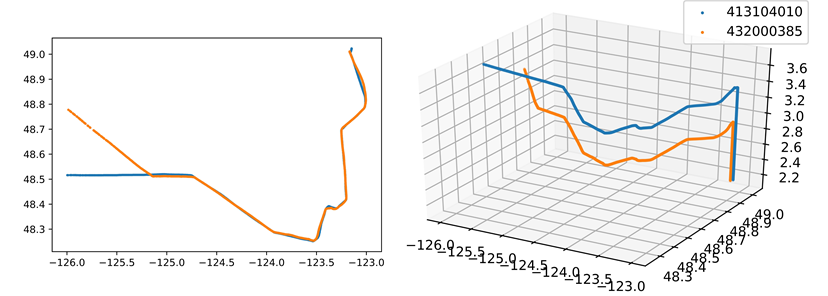
\includegraphics[width=\textwidth]{figures/Ch4/VesselRendevouz.png}
\caption{Routes of MMSI: 413104010 and 432000385; axes representing (lat.,long.)[Left]
and (lat.,long.,time)[Right]}
\label{fig: Ch4 VesselRendevouz}
\end{figure}




%-----------RB-ADS-----------

\section{Rule Based Anomaly Detection Service}
\label{section: 4 Rule Based Anomaly Detection}
A Rule is defined as something that can, at least in the way we approach them, be expressed as an if-then sentence, ~\cite{Edlund2006Rule-basedSurveillance}
Anomaly Detection based on the definition of rules, is extremely used in the literature, as it represents an effective way to detect Anomalies at seas. Although this in only viable if and only if the rules are defined by Subject Matter Experts (SMEs)~\cite{Boinepalli2014AAlgorithm, Will2011FastProcesses}.

Rule Based Anomaly Detection Service, was developed to detect Anomalies that can be codified into a rule or a set of rules, in real-time. 
Our approach to detect Anomalies in real-time was by storing the $N$ last Behavioural Points for each Vessel in a Service Cache, working like a first in first out (FIFO) queue. $N$ is a configurable Value, which represents the limit of messages stored in Service Cache for each Vessel, we provide an intuitively way to reduce the hardware requirements to run this service in Real-Time.

When the Service Cache has stored $N$ $BPs$ for a certain Vessel the Rule Based Anomaly Service is called for this Vessel, as demonstrated in Figure~\ref{fig: RB-ADS}, in Vessel MMSI n case.
If a Vessel queue has $N$ $BPs$, and was the Rule Based Anomaly Service was already called of this messages, all Vessel Service Cache being FIFO, we discard the oldest $BPs$, thus the Vessel Queue after is full for the first time it as always $N$.

\begin{figure}[H]
\centering
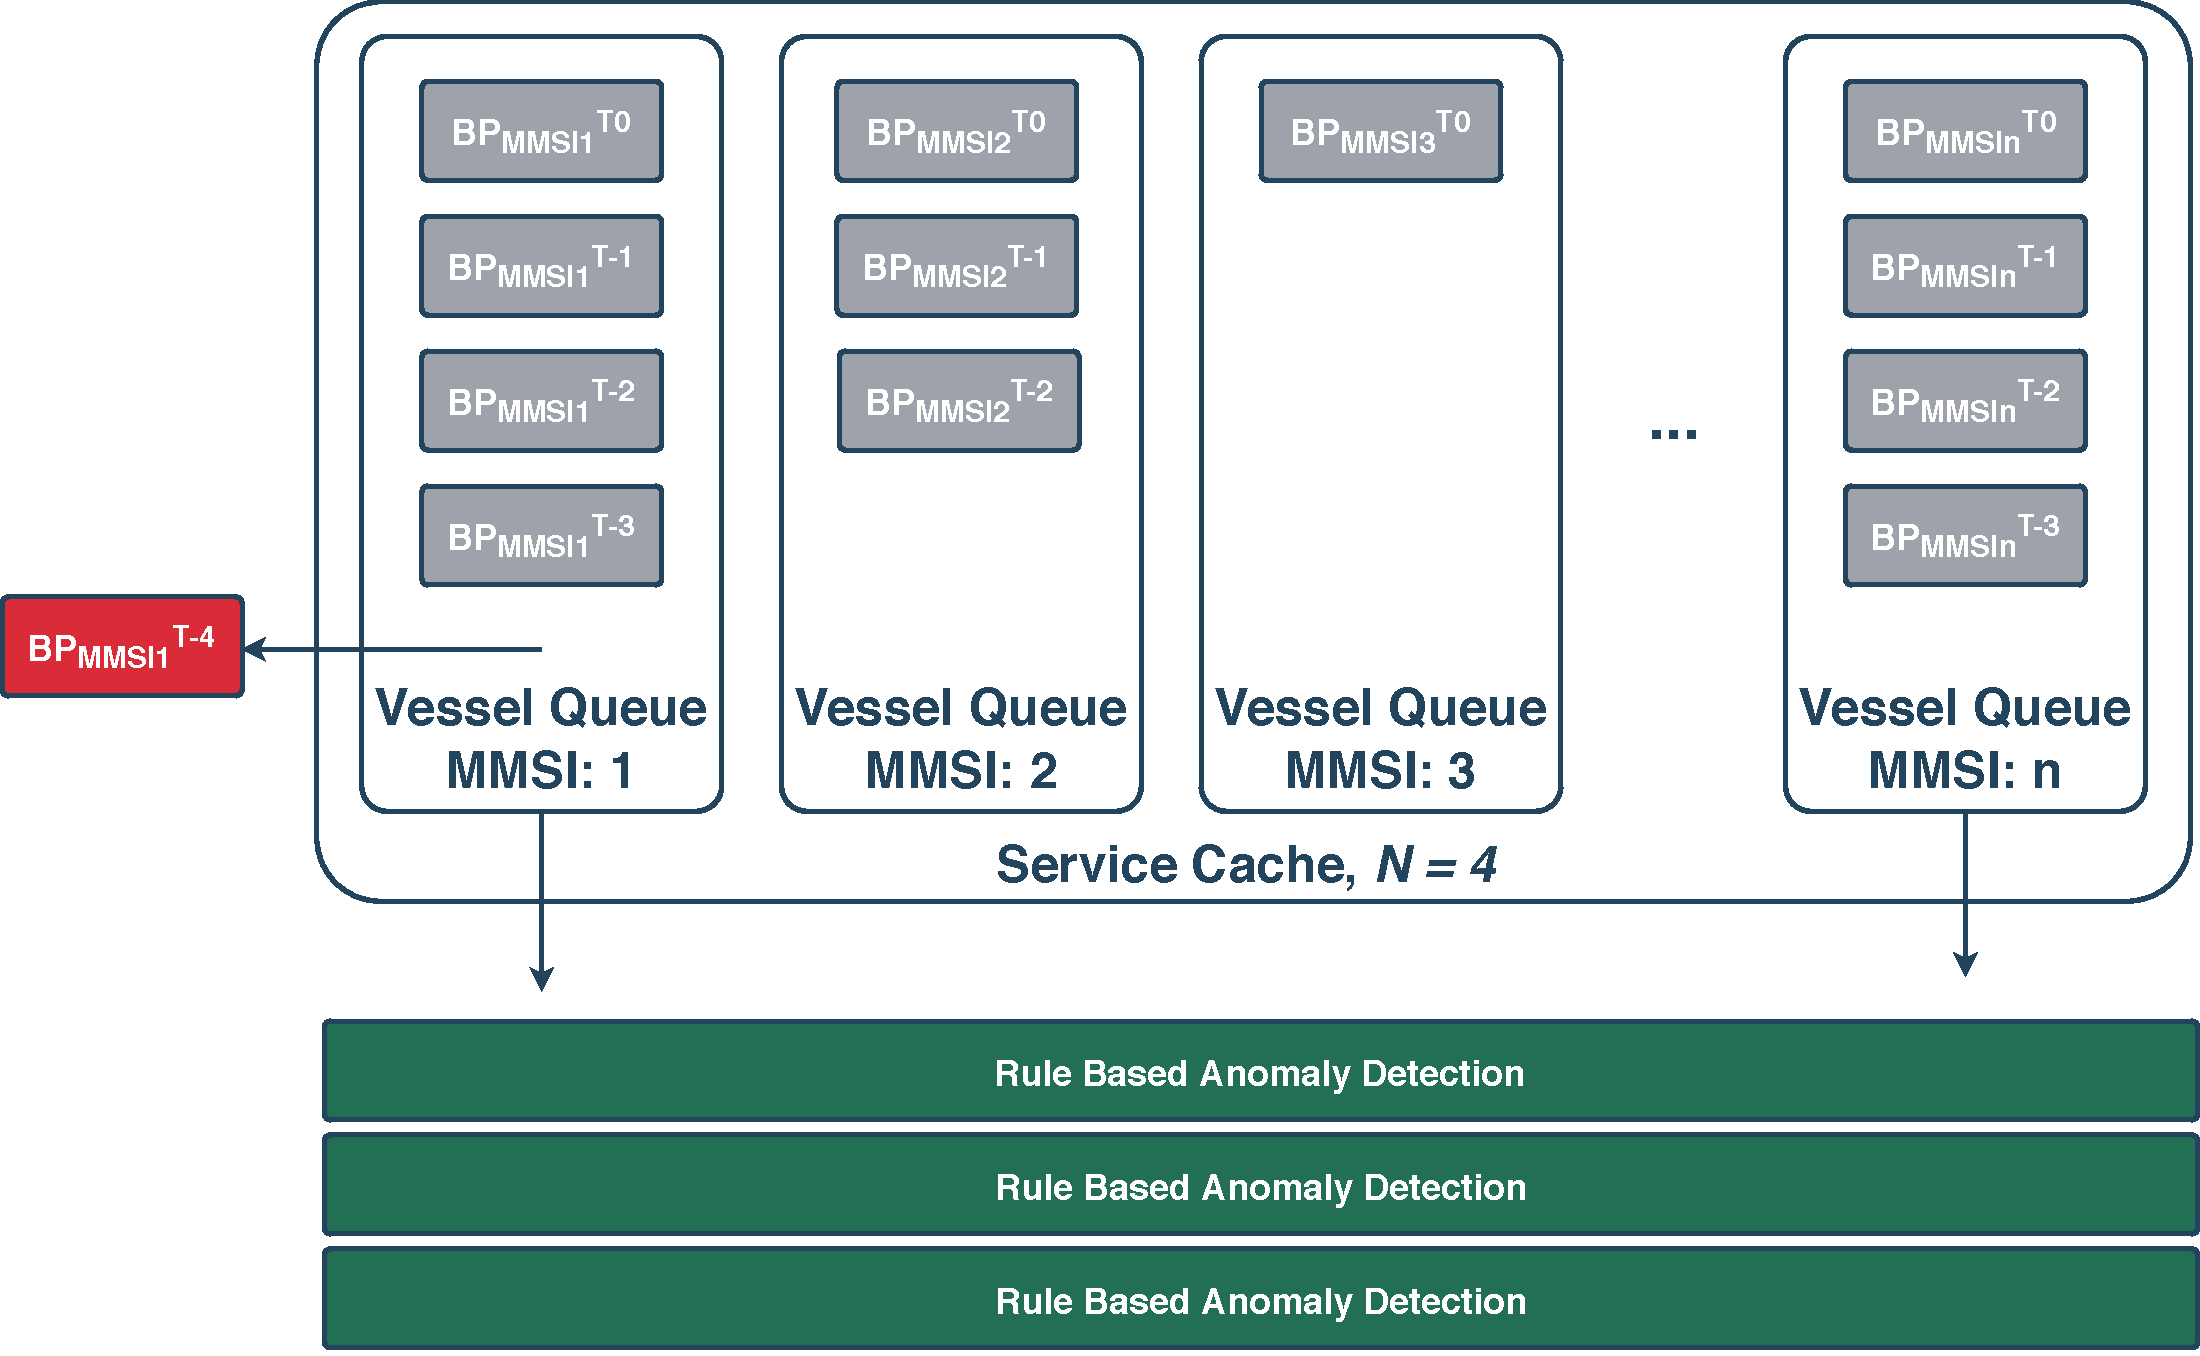
\includegraphics[scale = .36]{figures/Ch4/RB-ADS.pdf}
\caption{Demonstration of a possible cases for RB-ADS Service Cache coordinator.}
\label{fig: RB-ADS}
\end{figure}

Rule-Based Anomaly Detection Service, allows a detection of Anomalies based on little previous knowledge of each Vessel Trajectory. Despite the Service could be configured with any Rule that could be written for either Temporal, Spatial or Features based Rules, for example:

\textit{If Vessel MMSI: X in Zone: Y Stopped for more than M minutes then Report as Anomaly.}

For this work we decided to focus on the creation of configurable Rules that could detect the Anomalies presented in Section~\ref{section: Framework Requirements}, as were the Anomalies that would be Validated by Maritime Officers,  which we present in Subsections Under.

\subsection{Speed}
\label{subsection: 4 Speed}
Speed represents a Set of configurable Rules that were implemented to detect the Anomaly, $(AR_2)$, defined in Section~\ref{Table: Anomaly Requiremtens}.

Our first approach for the detection of an \textit{Abnormal Change of Velocity} was, calculating the $SoG$ difference from the latest received, $BP^T$ with the previous $BPs^{T-1}$, stored in the Vessel Queue.
If the difference is bigger than a defined $SoG$ $Treshold$, then an Anomaly is generated with the $BPs$ stored in the Message Queue, and the configurations that generated this Anomaly, which could be represented as:
\begin{align*}
\mathbf{if}\;\;& abs({BP_{MMSIn}}^{T}.SoG - {BP_{MMSIn}}^{T-1}.SoG) > SpeedThreshhold
\;\;\mathbf{then} \\ 
&Anomaly[{BP_{MMSIn}}^{T}, {BP_{MMSIn}}^{T-1}] 
\end{align*}
Although, calculating the $SoG$ difference was only viable if  $N = 2 $ was considered as the size of the Vessel Queue.
When considering more than two $BPs$ the difference is not representative of the actual \textit{Abnormal Change of Speed}, in order to mitigate this we created a new configuration, representing the operation it should be done in this case, which for this anomaly we considered the Average Difference, the Max Difference.

\subsection{Course}
\label{subsection: 4 Course}
Similar the \textbf{Speed} defined above, Course represents a Set of configurable Rules implemented for the Anomaly detection, of $(AR_1)$, which is the \textit{Detection of Abnormal change of Direction}. 
Our approach for the detection of $(AR_1)$ was quite similar to the {Detection abnormal change of Velocity}. 
Although, we noticed depending how Vessels are Moored at port\footnote{http://marineinsight.com/marine-navigation/mooring-methods-ships/}  Vessels tend to swing, due to the Sea Currents, or just from the movement of other Vessels moving in Ports. This creates abrupt changes of $CoG$, which are not representative of the Anomaly Requirement $(AR_1)$.

In order to mitigate this problem, we defined other configurable condition, Minimum SoG Threshold. Thus, the representation of the configurable Set of rules for the detection of rule for the detection of $(AR_1)$, is :

\[ If\; abs(MQ_{T}.CoG - MQ_{T-1}.CoG)\;and\; MQ_T.SoG > S\; then\; Anomalous.\]

\subsection{AIS Signal Loss}
\label{subsection: 4 AIS Signal Loss}
The \textit{disappearance from sensor coverage for more than a configurable Time Period}, $(AR_3)$, from a data stand point the is represented as the loss of signal, or in other words, the non reception of AIS messages from this Vessel for more than $M$ Minutes.

In this work, we detect the loss of signal from Vessel, by analysing when did a certain Vessel transmitted for the last time. This is done in real time, by the RB-ADS by one of two ways: the A priori way or the posteriori way.

First, as we store the Last $N$ $BPs$ for each Vessel that we received AIS messages from, in a the respective Message Queue from the Service Cache. By calculating the difference between the the last received ${BP_{MMSI}}^T$ to the ${BP_{MMSI}}^T-1$, we can know what was the elapsed time. Therefore, if this elapsed Time is bigger than a configurable Time $M$, this is reported as Anomaly. This method is considered a posteriori, as we are waiting for a new message to generate a Signal Loss Anomaly.

The a priori way, is when a Signal Loss anomaly is generated with out the reception of the a new message of a certain Vessel. Having the latest $BP$ for each Vessel stored in the Vessel Queue, if more than $M$ minutes have passed without receiving a Message for this Vessel an anomaly is generated. Both methods of detection represent the actual Signal Loss from a Data Stand point, and depending on the situation both can generate value to the End-Users. 


\chapter{MAD-F Evaluation}
\label{chapter:Chapter 5}
\lhead{Chapter 5. \emph{MAD-F Evaluation}}

In this Chapter, we present a group of experiments on the MAD-F capabilities. Firstly, we undertake data ingestion and storage performance test, which is followed by a exploratory analysis of the gathered data. Secondly we validate each of the ADS modules, starting with the RB-ADS Experiment, where the data that was collected previously is Experiment is injected in this module with the help of a simulator. After an Experiment over the ADS is conducted, where for each of the anomalies that are detected we provide and exploratory analysis of the results.
The \emph{validation} of the results presented in this Chapter, can only truly be done by Maritime Officer. What is to be called as anomalies in this work must not be interpreted as an actual maritime illegality, but only as a possible anomaly, which needs always to be validated by Maritime Officer. The real validation of the developed MAD-F will be done by the project end-users the Maritime Experts. \textsc{Marisa} being an highly collaborative and undergoing project, such validation at the time of writing this dissertation were still to occur. The validation of the MAD-F by the project end users is described under in Section~\ref{Section: 5 Marisa Validation}. 
All the experiments under in this Chapter were conducted on a Desktop PC using a Intel Core I5-7600k CPU with 16Gb of RAM.

\section{Data Ingestion Experiment}
\label{section: Experiment Data}
Data Ingestion Experiment refers to the Experiment were we accessed the performance of the Data-Ingestion capability of MAD-F. In order to achieve this, we provided a real NMEA feed as input to our the Data Ingestion Module. The NMEA feed was provided by the Portuguese Navy via the \textsc{Marisa} project, and this specific feed aggregated messages from multiple antennas around Portugal.
 
With the provided feed, we allowed the MAD-F to be executed for five straight days, thus ingesting pre-processing and wrangling the NMEA feed into Behavioural Points. As for this experiment we used a real NMEA feed, the messages were firstly decoded into a readable format, and only then after the whole pre-processing was done, the $BPs$ were stored in the Trajectory Extraction Cassandra Data-Base.

From the 5 days of data acquiring, we acquired from a total of $2,259,615~BPs$ from $5,563$ different Vessels.
As the provided feed did not broadcast any vessel static information, from the vessel that generated each message. The vessel static information namely the vessel type and country of origin, were scrapped from the internet using the developed \emph{Vessel Type Scrapper} which we presented in Section~\ref{subsection: Vessel Type}. 
From the $5,563$ vessels, $6$ of them were not considered for this Experiment. The MMSI of this vessels was either not found or their MMSI was representative for more than one Vessel. The latter, represents an abnormal situation which could be denominated Spoofing, as represented by the authors in~\cite{Ray2015DeAISRisks} or in \footnote{http://globalfishingwatch.org/data/spoofing-one-identity-shared-by-multiple-vessels}. This is a occurring problem when handling AIS data, and will be discussed in the future work.
In Figure~\ref{fig: 5 Vessel Type Distribution}, we present the vessel type distribution from the acquired $BPs$.
\begin{figure}[H]
	\centering
	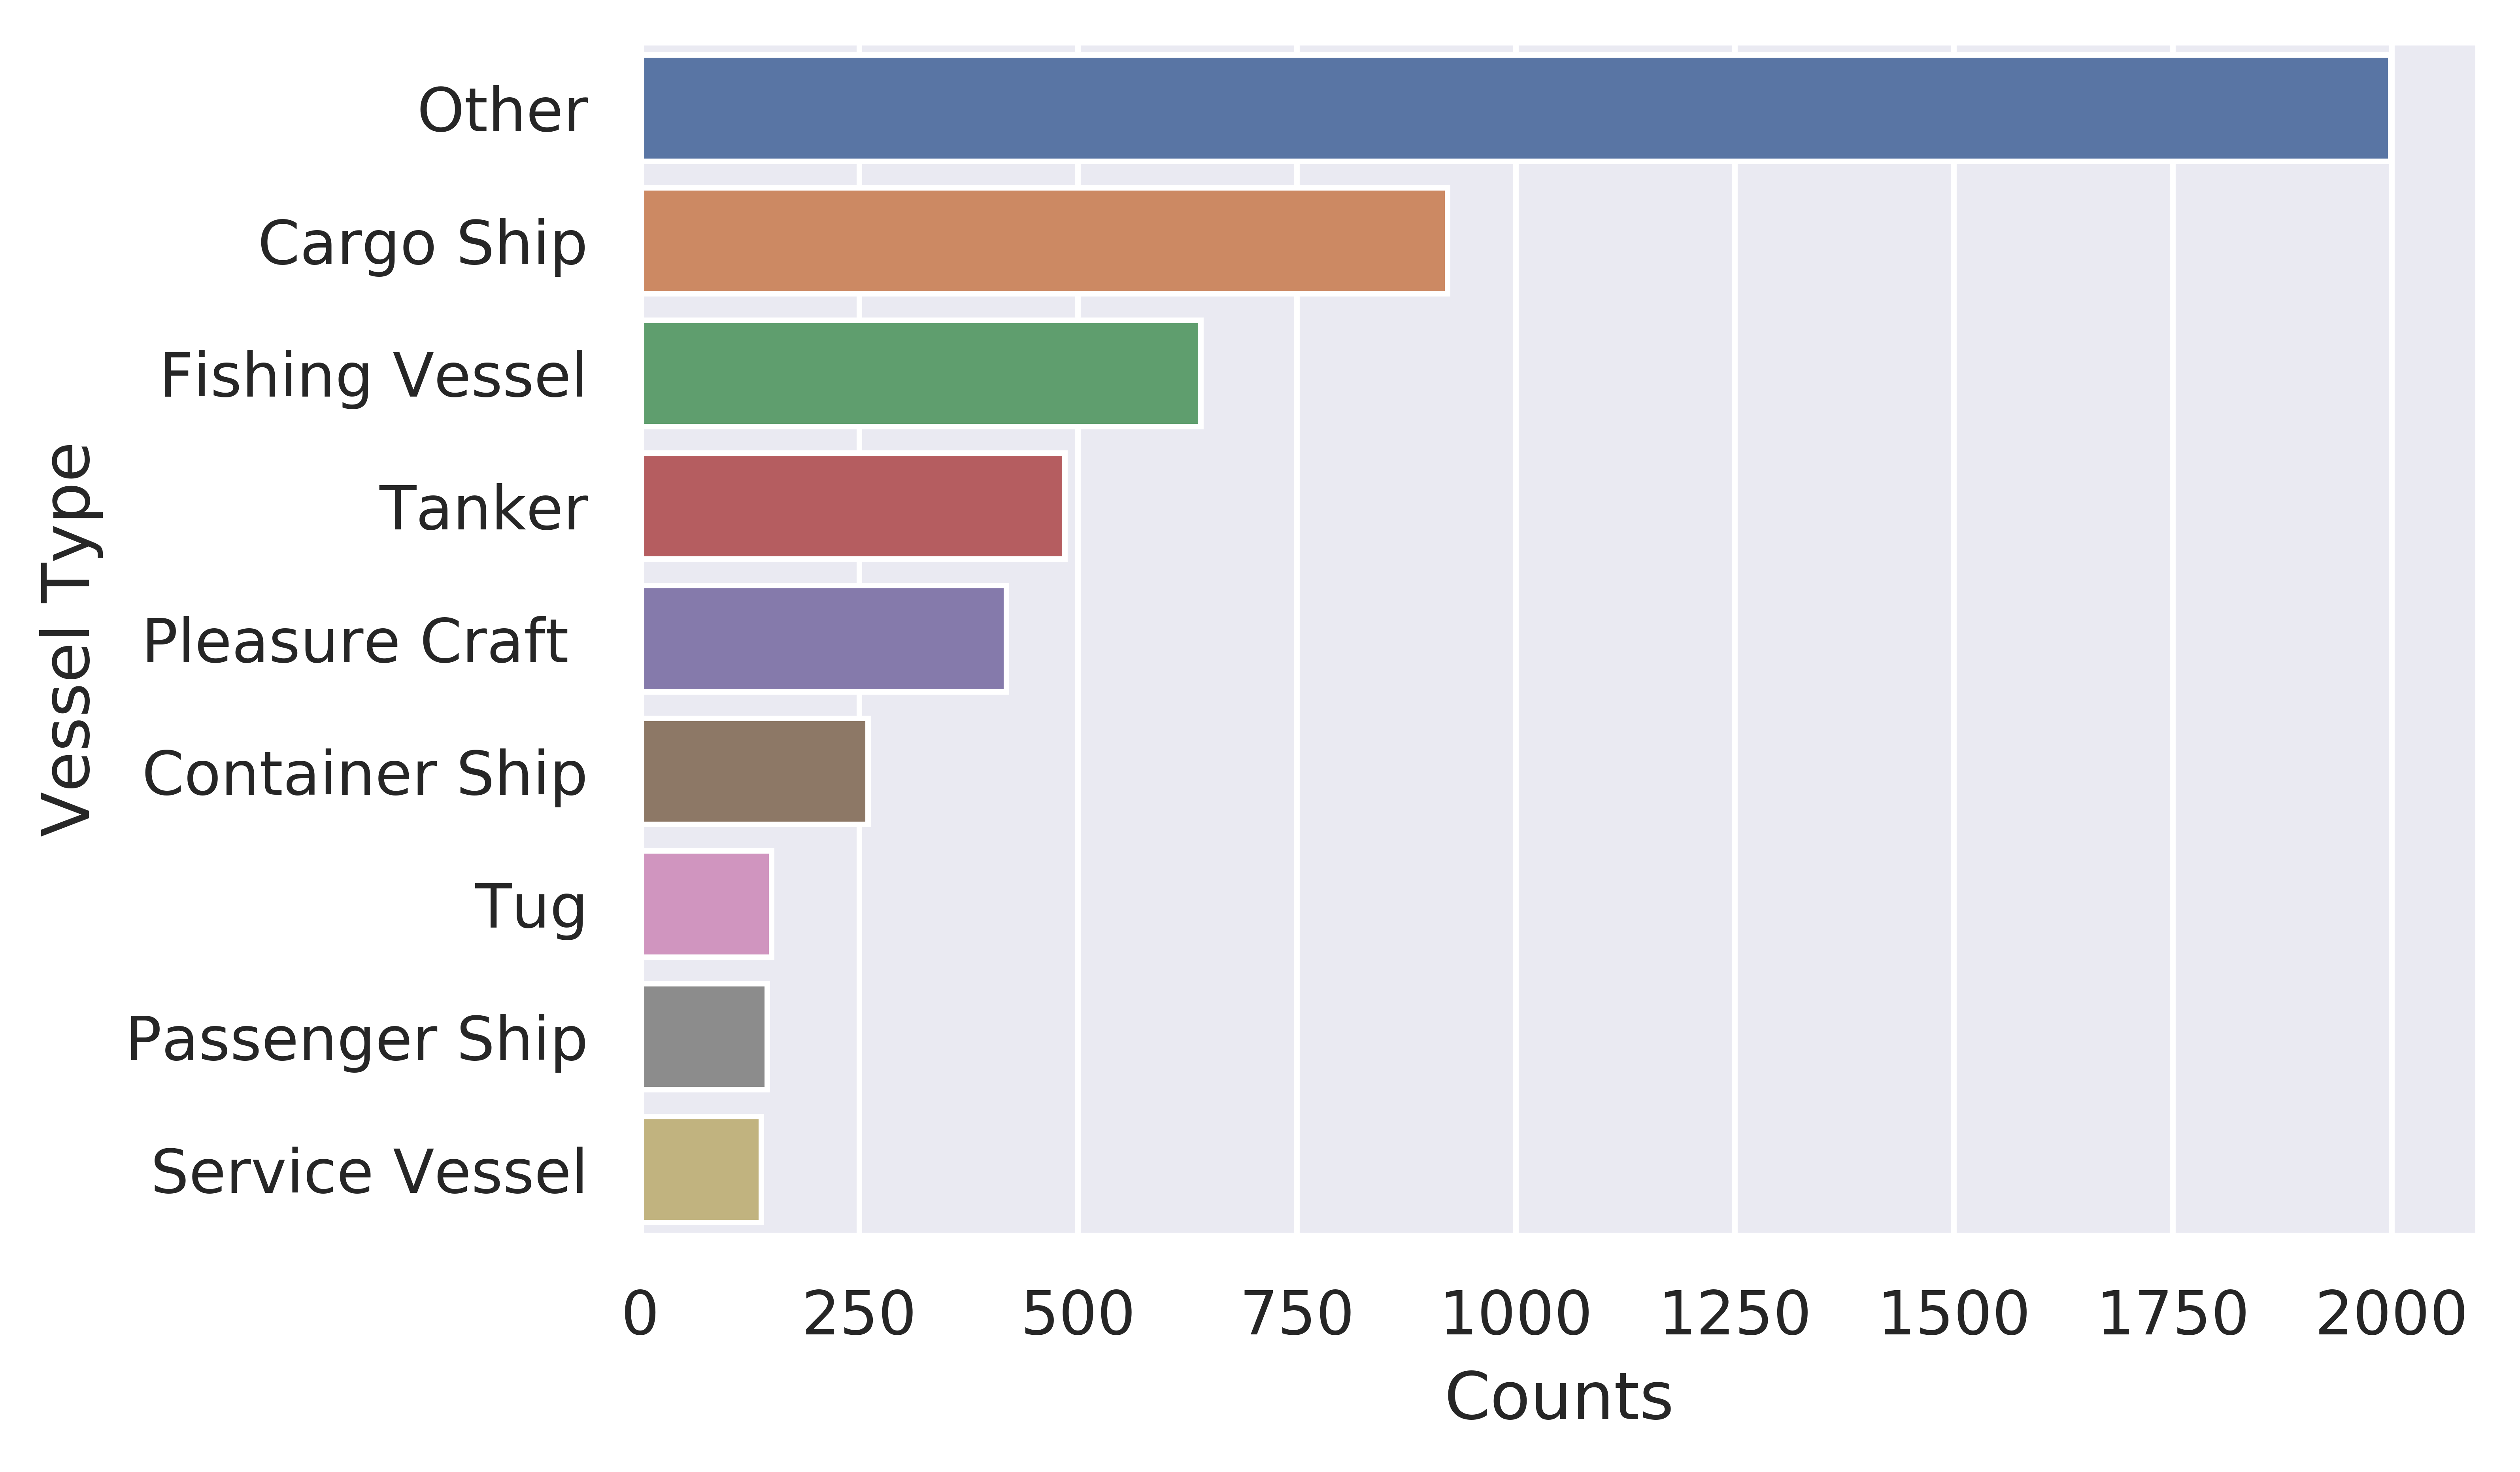
\includegraphics[scale = .7]{figures/Ch5/DataValidationVesselType.png}
    \caption{Vessel Type distribution of $5,157$ Vessels.}
    \label{fig: 5 Vessel Type Distribution}
\end{figure}

Another feature calculated while transforming data into $BPs$ was the point-based closest distance to coast and ports, which was done to every received NMEA AIS message received. In order to validate if this calculation were in fact being accurate, we analysed based on the received $BPs$ which countries were the closest and the respective ports.
In Table~\ref{Table: 5 Closest Countries} we present the distribution of closest countries. 
\begin{table}[H]
\centering
\caption{Most Frequent Closest Countries Counts.}
\label{Table: 5 Closest Countries}
\begin{tabular}{@{}lcc@{}}
\toprule
Country & Counts & Counts(\%) \\ \midrule
Spain & 1,306,436 & 58\% \\
Portugal & 663,841 & 29\% \\
Morocco & 259,776 & 11\% \\
Gibraltar & 26,885 & 1\% \\
France & 2,516 & 0.1\% \\ \bottomrule
\end{tabular}
\end{table}
In Table ~\ref{Table: 5 Closest Ports} we present a post validation of the closest Ports for every received message. This was done as a way to analyse if based on the the closest country the most closest ports seems plausible, as a individual message validation would be impossible. Thus, under we present a subset of top most frequent closest ports from the $69$ total possible Ports found in the data.
\begin{table}[H]
\centering
\caption{Most Frequent Closest Ports Counts.}
\label{Table: 5 Closest Ports}
\begin{tabular}{@{}lcc@{}}
\toprule
Port Name & Counts & Counts(\%) \\ \midrule
Lisboa & 142,464 & 6,3\% \\
Villa Garcia De Arosa & 112,254 & 5\% \\
Europa Point(Gibraltar) & 109,273 & 4,8\% \\
Lagos & 107358 & 4,7\% \\
Las Palmas & 106,116 & 3,5\% \\
Cadiz & 79,577 & 3,5\% \\
La Corunha & 78,929 & 3,5\% \\
Malaga & 65,227 & 2,9\% \\
Vigo & 64,759 & 2,9\% \\
Faro & 62,925 & 2,9\% \\ \bottomrule
\end{tabular}
\end{table}

By displaying all the 2.2 Million $BPs$ into a density plot, we try to positional occurrence of the transmitted messages. As scattering Millions of points is computational heavy, and if "normal" plotting packages were to be used not possible with the Hardware specifications presented in the begining of this Chapter. Thus the density plots presented in this Chapter were using the~\footnote{http://vaex.astro.rug.nl}, which is optimised huge datasets. 

\begin{figure}[H]
	\centering
	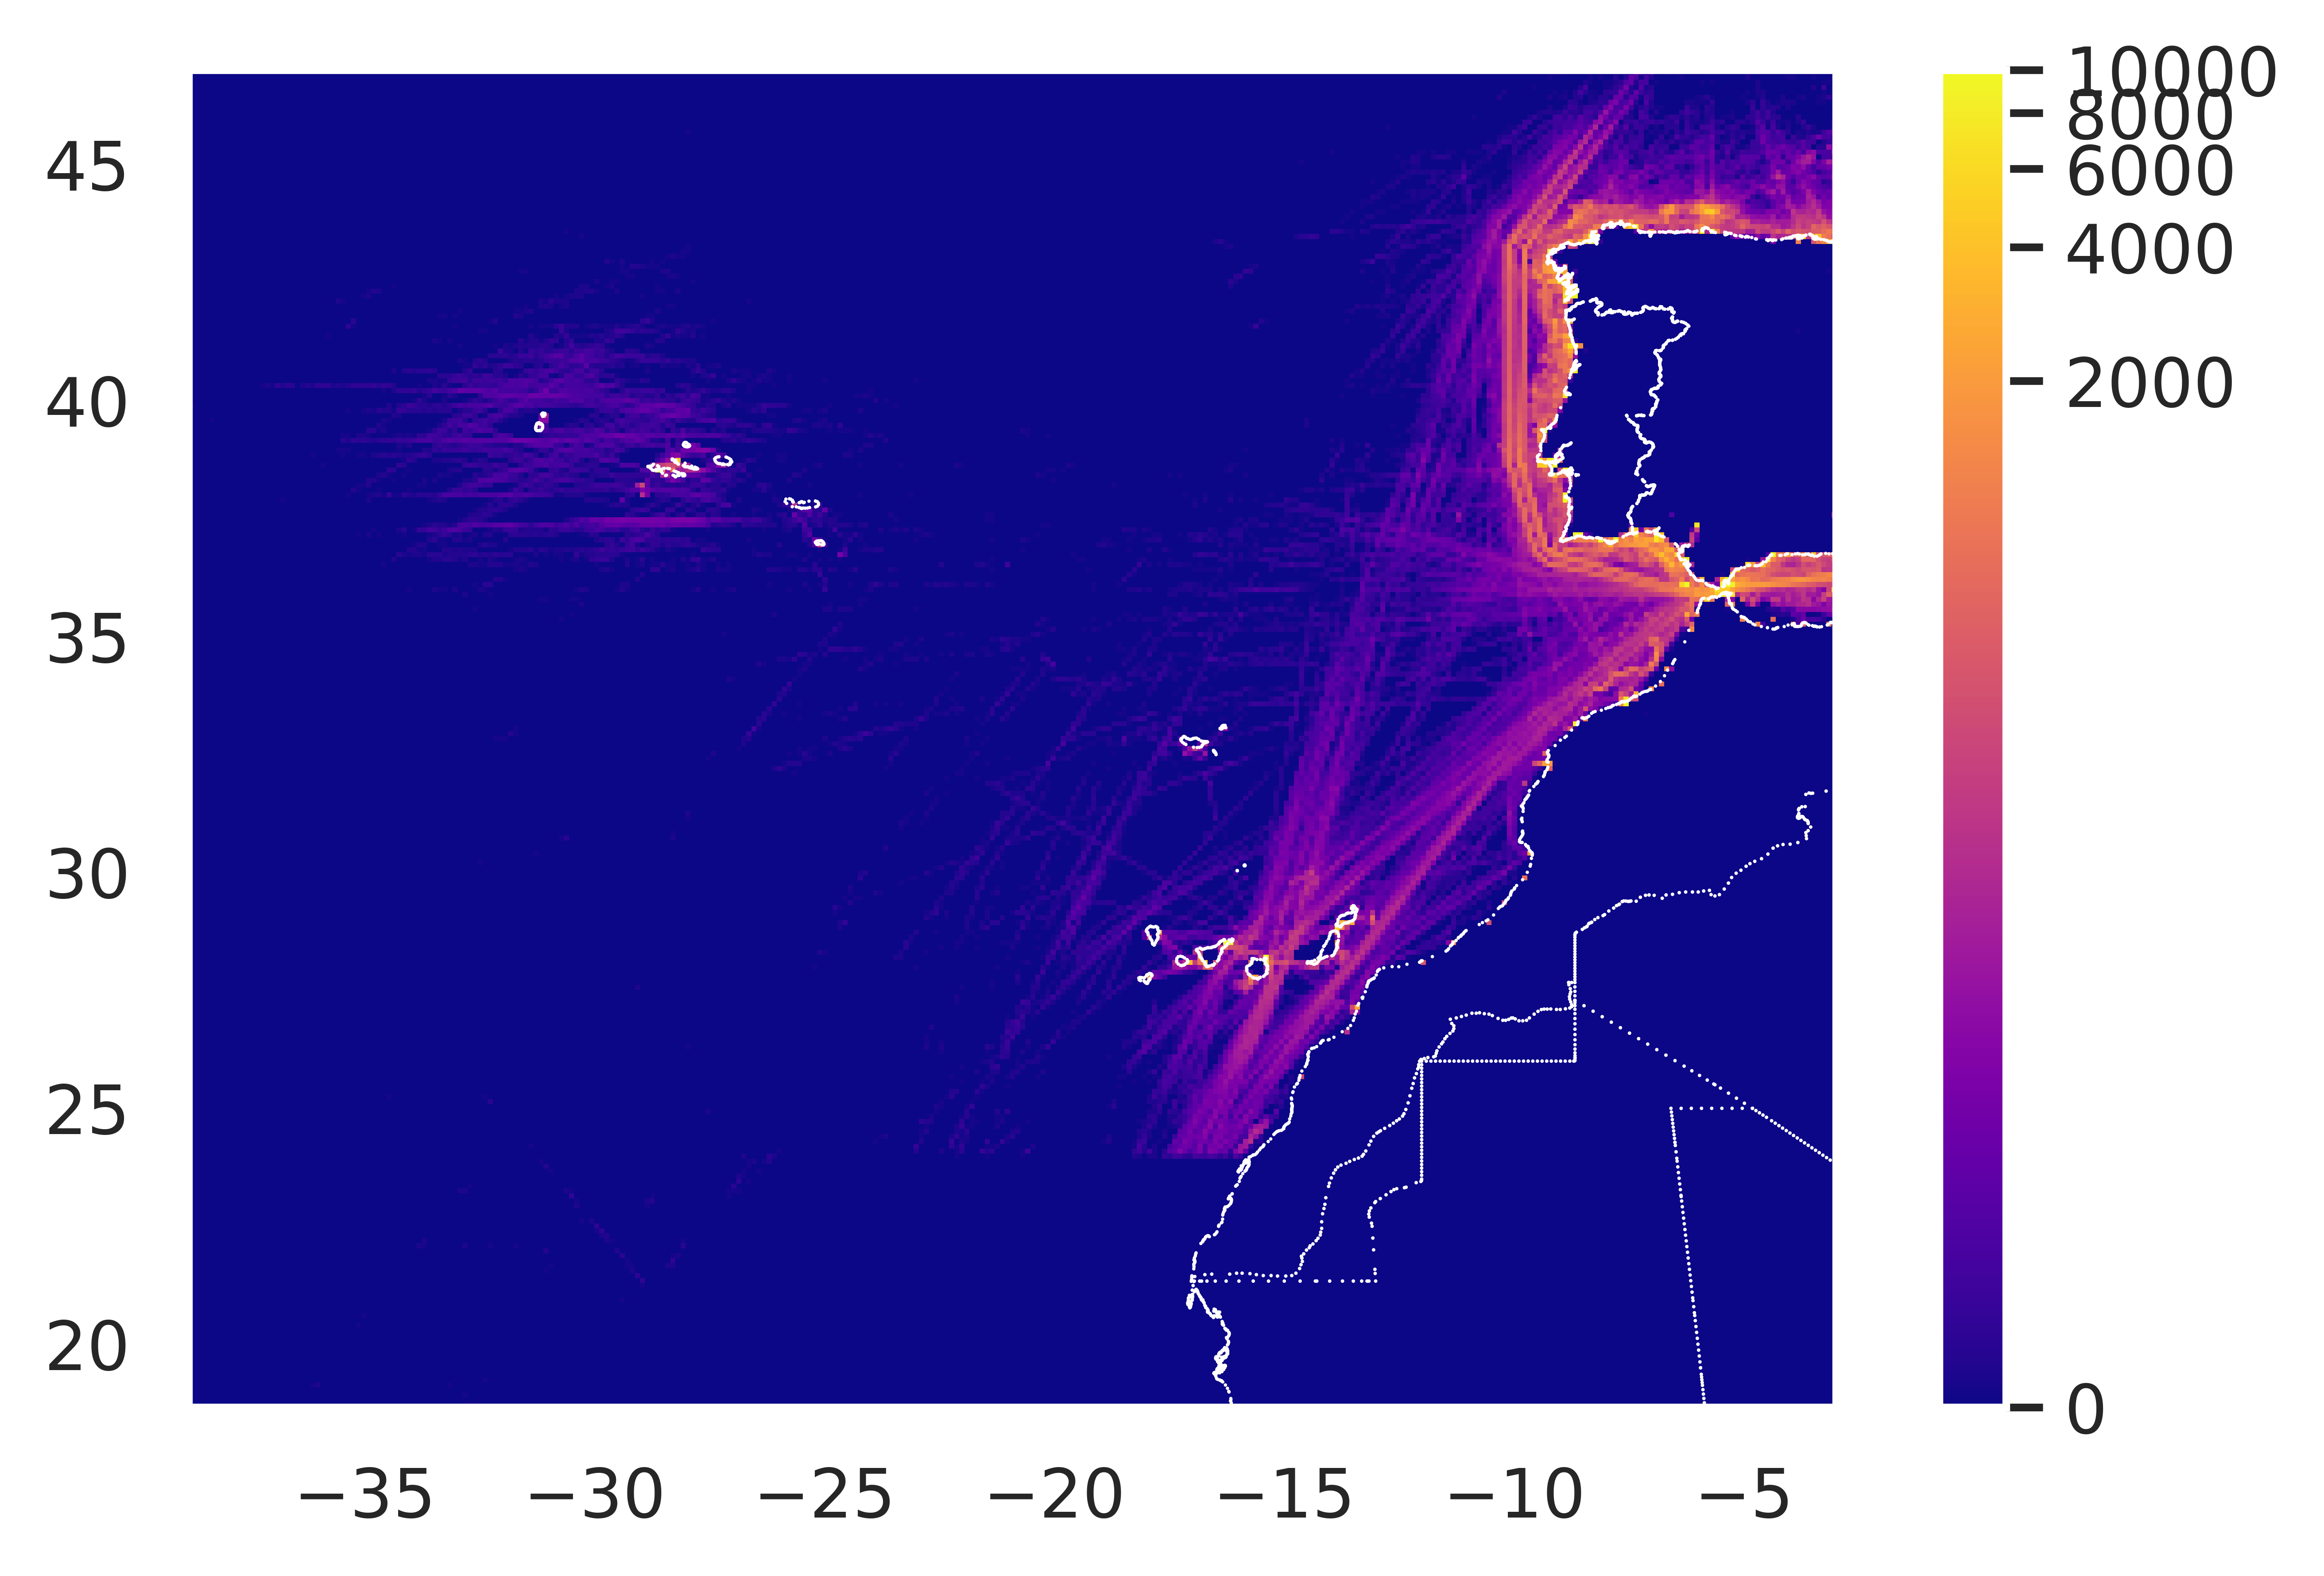
\includegraphics[width=\textwidth]{figures/Ch5/ThesisExpDensity.png}
    \caption{Density map, with all the approximately
    $2.2$ Million points.}
    \label{fig: 5 Exp1DensityMap}
\end{figure}

What we found by analysing Figure~\ref{fig: 5 Exp1DensityMap} is that in fact the messages that were received via the Portuguese Navy antennas. Which explains the reception of messages near the Madeira and Azores islands.  What is possible also to analyse in the Figure, is nearby the Portuguese coastal line a few lines of high density traffic show up. These lines represent the navigational lanes, and when navigation in this lanes vessels tend to have a more standardised behaviour. Such fact can be explored other types of AD, and is presented by the authors in~\cite{Yan2016} and~\cite{Silveira2013UsePortugal}. The acknowledge of this lanes for anomaly detection will be endorsed in future work.


\section{RB-ADS Experiment}
\label{section: RB-ADS Experiment}
This experiment was conducted, in order to validate the real time capacities of the RB-ADS Module. In order to validate such capacities, we focused this experiment on the validation by analysis of the anomalies which were generated, and whether this anomalies were generated in near-real time.
This experiment was simultaneously conducted as the previous Experiment~\ref{subsection: Data Ingestion}. This was possible as the incoming messages after being ingested and pre-processed they were stored in the Trajectory Extraction module as $BPs$ but simultaneously the same $BPs$ were inputted in the RB-ADS module.
The RB-ADS module managed the incoming $BPs$, using the implemented service queue, which we explained in~\ref{section: 4 Rule Based Anomaly Detection}. For this experiment we set the service queue $N$, size to \textbf{$2$}. This made the anomaly detection be executed, if any vessel queue had two $BPs$, with the set of rules, which we defined and are represented under in Table~\ref{Table: 5 exp. RB-ADS rules}. 

\begin{table}[H]
\centering
\caption{RB-ADS Experiment, rule configurations, where the columns represent the variables.}
\label{Table: 5 exp. RB-ADS rules}
\begin{tabular}{@{}ccccc@{}}
\toprule
Rule & SOG variation & GOG variation & SOG min. & Time Elapsed \\ \midrule
R1 & - & - & - & 15min. (post.) \\
R2 & \textgreater{}15 knot & - & - & - \\
R3 & - & \textgreater 25º & \textgreater 0.5 knot & - \\ \bottomrule
\end{tabular}
\end{table}

From the 5 days of executing the MAD-F, as mentioned in Section~\ref{section: Experiment Data} a total of $2,259,615 BPs$ were processed and ingested in the RB-ADF modules. With the presented set of rules a total of $191,481$ anomalies were generated. These number of anomalies is rather large, representing approximately $8\%$ of all the $BPs$ were considered anomalous for one of these rules. In Table~\ref{Table: 5 exp. results rules} we detail more explicitly the total number of anomalies by analysing the rules which generated such anomalies. As well as the matching the defined rules for this Experiment with the anomaly requirements, which were defined in~\ref{section: Framework Requirements}.

\begin{table}[H]
\centering
\caption{Anomalies found for each Rule with the respective Anomaly Requirement.}
\label{Table: 5 exp. results rules}
\begin{tabular}{@{}ccccc@{}}
\toprule
Rule & R1 & R2 & R3 & Total \\ \midrule
Count & 82,866 & 2,144 & 106,471 & 191,481 \\
\begin{tabular}[c]{@{}c@{}}Anomaly\\ Requirement\end{tabular} & AR3 & AR2 & AR1 & - \\ \bottomrule
\end{tabular}
\end{table}

From the results presented above what is possible to analyse, is that the most occurring anomaly was the abnormal change of direction this despite the filtering of normal course variations on vessels which were stopped. We further analysed the time difference between same vessel transmissions. What we found out was that the \emph{mean transmission rate}, was of approximately \textbf{10min.}, which is high for a real AIS feed. Although, if the $BPs$ which were considered anomalous from the $R1$, were not considered for the calculation of this mean, the \emph{mean transmission rate} would be \textbf{5min.}. Thus, if a new rule were to be applied where from the $R3$ only messages that had been transmitted with a time difference inferior to 5 minutes, which could be represented as  $COG.diff>25~and~TimeDiff.<5minutes$, only \textbf{7} anomaly occurrences would occur.

The additional rule presented above, was not validated with the live NMEA feed, as this was a live stream. Nevertheless, this rule was still validated with the same data. As the results from the Experiment~\ref{section: Experiment Data} were stored in the trajectory data-base, these could be accessed multiple times. For the purpose of these current work we developed a $BPs$ simulator which from the stored trajectories would simulate the real reception of AIS streams (from the perspective of the RB-ADS module).

The simulator gathers $BPs$ from the trajectories (or a group of) stored in the trajectory data-base, and send this $BPs$ to the RB-ADS, as presented in~\ref{fig: 5 BPs Simulator}.
\\
\begin{figure}[H]
	\centering
	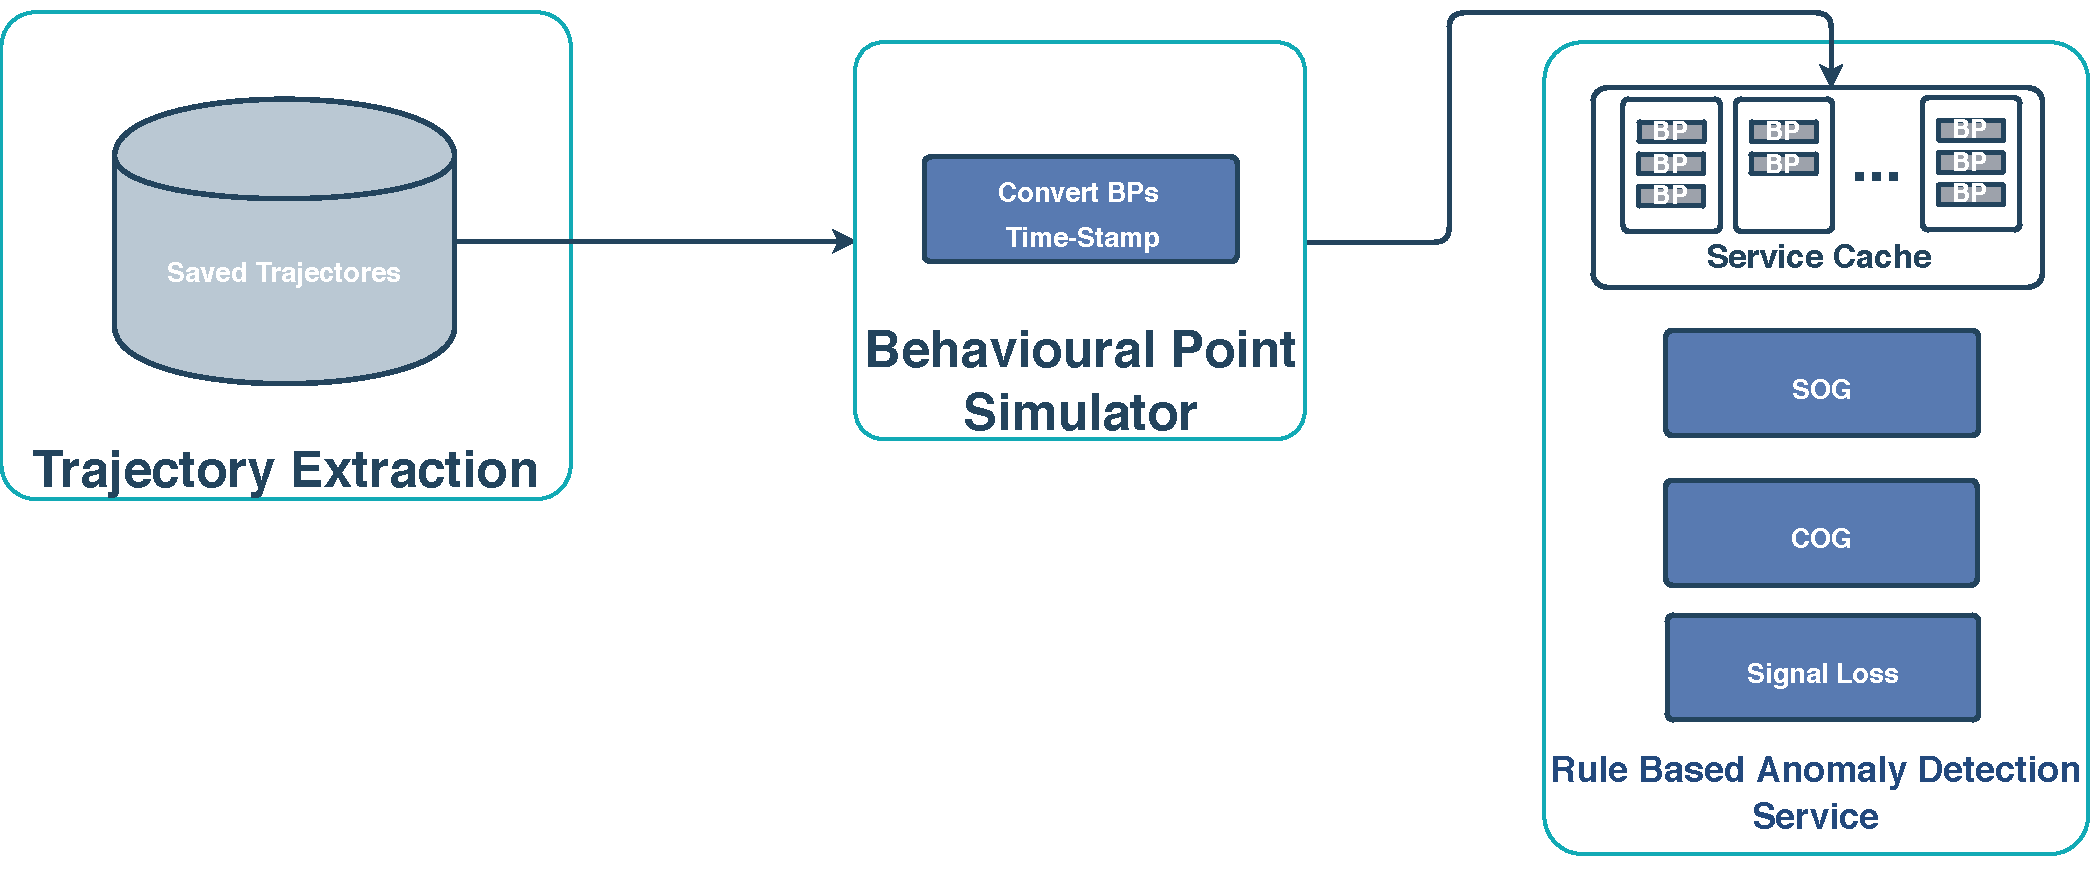
\includegraphics[width=\textwidth]{figures/Ch5/SRM-Exp-Simulator.pdf}
    \caption{BPs Simulator.}
    \label{fig: 5 BPs Simulator}
\end{figure}

The simulator worked by setting the a \textbf{Initial-Simulated-Time} as if it was the current Time. This time was the first time-stamp of the stored $BPs$. Based on this \textbf{Initial-Simulated-Time}, the following $BPs$ would be sent based on the time difference from this \textbf{Initial-Simulated-Time}. As it would be impractical to wait 5 days for the simulation of the reception of this data, the developed simulator was implemented with a \emph{speed up factor}. This some what allowed us to replicate the real reception of the same data, while simultaneously analysing the results of different rules.

\iffalse
Thus, using the $BPs$ simulator additional rules could be applied with the same data, thus gaining insight on the generated anomalies. 

which were considered anomalous for $R1$ were not considered in $R3$, which would be the same as defining a new rule that would be $COG.diff>25~and~Time$ which we gonna name \textbf{$R4$}.
If $R4$ would be applied on the same data, only   

As new $BPs$ were being created by the MAD-F, from the NMEA feed, the RB-ADS module was generating anomalies, based on the rules previously defined. This in the end generated a total of XXX anomalies, which we detail in Table XXX.

\todo[inline]{SEE IF I WANT TO TALK ABOU THE MEADIAN TIME ETC ETC...}

was acquiring messages from the NMEA feed, the
we injected the resulting $BPs$ from the Experiment~\ref{section: Experiment Data} in the RB-ADS module. Therefore this experiment was not conducted using the real-time data NMEA feeds. If the feed would be used,  we would loose control of the incoming data, which would make this experiment not possible to replicate.

For this Experiment the \textbf{Initial-Simulated-Time} was set first received $BP$ from the Experiment~\ref{section: Experiment Data}, which was XXXXXXTODOXXXXXX.  

As it would be not practical waiting 5 days for this Experiment, we 
Thus, we ran RB-ADS with the simulator setted to a speed of X. 

The RB-ADS was then executed with the set of rules represented under in Table and with the RB-ADS parameters represented in Table~\ref{Table: 5 exp. RB-ADS rules}.


With the parameters described above, we generated a sum of XXX anomalies from the 3 rules used, as detailed in table XX. 
\fi

\section{Anomaly Detection Service Experiment}
\emph{ADS Experiment} for this current work represents our validation process of the developed offline AD functionalities. The steps towards this experiment were similar to the Experiment~\ref{section: RB-ADS Experiment}. As this module was developed to access more complex anomaly detection methods by the use of batches of historical data. We did not conduct this experiment same data as presented in~\ref{section: Experiment Data} or had a similar approach as for the Experiment~\ref{section: RB-ADS Experiment}.
As we already had preconceived knowledge of the dataset which we used in our initial data-analysis (Section~\ref{section: Data Analysis}). We conducted this Experiment with the same dataset, as it in fact represented an huge batch of historical data.
presented an huge batch of data. 

Before performing of the \emph{ADS Experiment} itself, the raw dataset was injected in the MAD-F as a single batch of data. This transformed a the historical AIS dataset into a normalised set of $BPs$, which was kept stored in \emph{Trajectory Data-Base}. What is to note is that if this group of $BPs$ were to be stored as files, these files would be nearly 5 GB(if stored as .csv type files).
As the transformation of the dataset in $BPs$ made the dataset pass through the "pre-processement" pipeline. This cleaned the whole dataset which was of initially 18,84 Million rows (AIS messages), from 4555 different Vessel, into approximately 17,10 Million $BPs$.
After the $BPs$ were store as trajectories, and additional "manual" filtering was done. We filtered the trajectories with a size inferior of 100 $BPs$. This filtering only slightly reduced the number of total $BPs$ considered for this experiment to 17,06 Million, although the number of considered Vessels was dramatically reduced to 1588 Vessels.

The ADS experiment was divided into two Sections. The first section presents the results obtained for the Vessel Rendezvous detection, and the second section presents the results for the Incoherent Navigational Status and Time Space incompatibility. The results are presented as the generated anomalies from the ADS module. From each subsection we present an explanatory analysis of the generated anomalies.  

\subsection{ADS - Rendezvous Experiment}
\label{subsection: ADS - Rendezvous Experiment}
This subsection, shows the results and our analysis of the results obtained from the Rendezvous sub-experiment. This sub-experiment was conducted on the the historical batch of data which was described above. The Rendezvous detection, as any other module of the proposed MAD-F was developed to be configured with the set of parameters most adequate for the situation which would be deployed. This choice of parameters in any real scenario would be done by Maritime Experts. Although for the sole purpose of this Experiment, the choice of parameters was done by us. This Experiment was conducted with four different sets of configurations(Table~\ref{Table: 5 ADS Rendezvous input paramenters}).

\begin{table}[H]
\centering
\caption{Anomaly Detection Service - Rendezvous input parameters.}
\label{Table: 5 ADS Rendezvous input paramenters}
\begin{tabular}{@{}cccc@{}}
\toprule
Rendezvous Parameter & BPs & Time-Window & Distance Threshold \\ \midrule
C1 & 17.1M & 10 min. & 50 yards \\
C2 & 17.1M & 2 min. & 50 yards \\
C3 & 17.1M & 10 min. & 10 yards \\
C4 & 17.1M & 2 min. & 50 yards \\ \bottomrule
\end{tabular}
\end{table}

The four different set of configurations were chosen in order to demonstrate the rendezvous anomaly detection capabilities. By varying the configuration the rendezvous detection can either be done in a more precise way, or in a more efficient way. The variation of \emph{Time-Windows} directly impacts the granularity of the detection and the variation of the \emph{Distance Threshold} impacts the proximity the vessels were to each other. In the Table~\ref{Table: 5 ADS Rendezvous results} we present the results obtained with the configurations presented above.

\begin{table}[H]
\centering
\caption{Rendezvous experiment results, with the variation of the configuration parameters. }
\label{Table: 5 ADS Rendezvous results}
\begin{tabular}{@{}cccc@{}}
\toprule
Parameters & Rendezvous Detected & Time Groups & Time Elapsed (aprox.) \\ \midrule
C1 & 35,667 & 131,760 & 50s \\
C2 & 120,773 & 26,352 & 4min. \\
C3 & 5,704 & 131,760 & 2min. \\
C4 & 18,993 & 26,352 & 40s \\ \bottomrule
\end{tabular}
\end{table}

From the results presented above, the first thing we noticed was that the number of occurrences was larger than expected. Regarding the variation of configurations what was found out, was that the variation of distance threshold impacts the number of possible rendezvous detentions, which was expected.
What was not expected was the number of occurrences increasing with the decrease of the time-groups sizes. 
Although, after analysing the results, this results did exactly what the method was developed for. As for this work, we considered an anomaly to be a single instance in time, and not the time group of which the anomaly had occurred. When considering lower time-groups sizes if two vessels had report twice in same position, two anomalies would be created. For the purpose of this analysis, and in order to mitigate this duplication of technically the same anomaly, thus gaining insight of how many rendezvous had occurred. We grouped the anomalies, therefore, if the anomalies were generated by the same group of vessels, in consequent time-groups they would be considered the anomaly with same with a larger duration. 
What was discovered from this grouping of consequent anomalies was that, with the configuration parameters \textbf{C4}, only \textbf{75} combinations of two vessels generated rendezvous anomalies. Although each combination of vessels generated multiple times rendezvous occurrences, with some combinations generating up to \textbf{7,436} times.

After analysing the frequency of occurrence, we analysed the location where the possible rendezvous had occurred. This led us to conclude that most of the detected rendezvous occurrences occurred nearby port.
As the only truly way to validate the results was by providing this results to a Maritime Officer which could not be achieved for the sole purpose of this present work. We decided to represent the Rendezvous occurrences which we detected on a distance of above 2 Km of the closest Port, thus creating a footprint of the possible Rendezvous occurrences for the whole dataset. A similar analysis is done by the authors in~\cite{Miller2018IdentifyingBehavior}. 

In Figure~\ref{fig: Chapter 5 Rend2Mapsr}, we present the a visual representation of the locations where the Rendezvous anomaly occurrence, from the area near the port of Brest(France). By displaying only the rendezvous events that occurred 2Km away from the closest port, the number of rendezvous occurrences is significantly reduced, it is possible to visualise in Figure~\ref{fig: Chapter 5 Rend2Mapsr}(Right). Nevertheless, as the a port for this work was considered as a single point, and a port can be way larger than just a single point. Filtering by the distance to port, by just considering as a point can cause a occurrence to not be filtered as sill in port. This problem will be addressed for Future Work.


\begin{figure}[H]
	\centering
	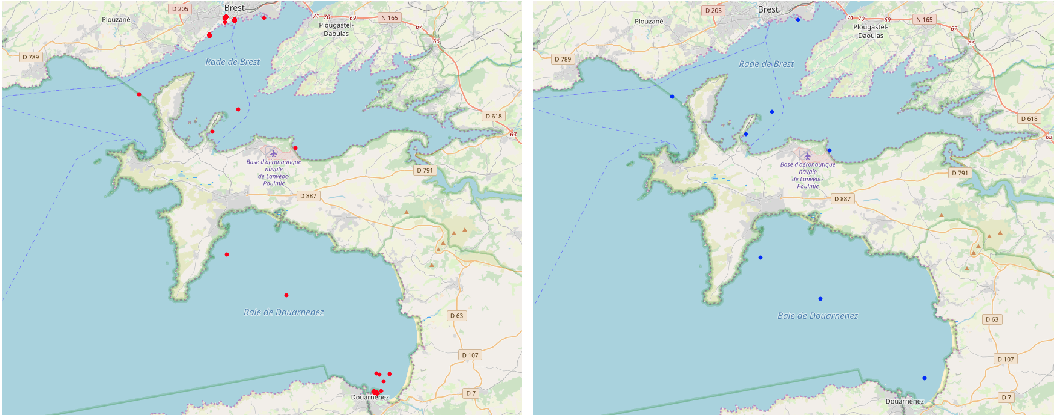
\includegraphics[width=\textwidth]{figures/Ch5/ThesisExpRend.pdf}
    \caption{Rendezvoused results, on the left no distance filter is applied and in right 2Km distance to port is applied.}
    \label{fig: Chapter 5 Rend2Mapsr}
\end{figure}


%As vessels being close to each-other inside a port is not anomalous, and brings no value to the Maritime Officers, we analysed the distance to port from the detected rendezvous occurrences. 
%In TableXXXX%~\ref{Table: 5 Distance to Port Rendevouz} we present the distance distribution, from the.
%The occurrences based in the Distance to Port, show that 20\% of the detected Rendezvous occurrences occur at Distance less than 500 Meters to Port. 

\subsection{ADS - Time Space Incompatibility Experiment}
\label{subsection: ADS - Time Space Incompatibility Experiment}
The time space incompatibility Experiment, serves for this present work as a Experiment in which we analyse the results from the ADS time-space incompatibility anomaly detection module. In order to achieve this, we took two different analysis for the this Experiment. First we analyse the overall anomalies generated, by varying the input parameters of this service. Secondly, as this service represents a some what first approach towards a vessel positional estimation, we applied the implemented linear estimation to the vessel trajectory, which was presented in~\ref{subsection: 4 Time-Space Incompatibility}, to a single trajectory which was presented in~\ref{subsection: Trajectory Definition}.

By following a similar approach as the one presented for the rendezvous Experiment, we used the historical batch of data previously described also for the detection of the space time incompatibility. As the \emph{Distance Factor Threshold}, is the configuration parameter for this specific anomaly detection, and it should be configured by a Maritime Expert depending on the scenario. For this Experiment we varied the $dft$ and analysed the results.  In Table~\ref{Table: 5 Time Space} we present the number of occurrences of the what was interpreted for this present work as the \textbf{AR5}(presented in Section~\ref{section: Framework Requirements}). 

\begin{table}[H]
\centering
\caption{Time space incompatibility occurrences, by varying the $dft$, and comparing with the $BP$ time shift.}
\label{Table: 5 Time Space}
\begin{tabular}{@{}cccccc@{}}
\toprule
Distance Factor Threshold & Delta Time & \textless{}2min. & \textless{}5min. & \textless{}15min. & \textgreater{}15min. \\ \midrule
500m & 6,581 & 391 & 866 & 1,978 & 4,559 \\
1km & 4,289 & 187 & 229 & 685 & 3,569 \\
2.5km & 2,373 & 53 & 53 & 95 & 2,257 \\
5km & 1,353 & 38 & 38 & 40 & 1,295 \\ \bottomrule
\end{tabular}
\end{table}

What was expected from this anomaly detection, was that the number of detected anomalies would increase with the decreasing of $dft$, this was confirmed by our Experiment. From this conclusion we further analysed this results by comparing the number of detected anomalies with the time shift from the previous $BP^{T-1}$, as we described in Section~\ref{subsection: ADS - Time Space Incompatibility Experiment}.
What is possible to analyse is the correlation from the time elapsed with the number of detected time space incompatibility occurrences. Thus, an Signal Loss Anomaly would also trigger a time space incompatibility anomaly.

Additionally for this Experiment, we applied the enriched Linear Estimation Equation which was presented in Section~\ref{subsection: 4 Time-Space Incompatibility} to a single trajectory of a Vessel, as we present under in Figure\ref{fig: Chapter 5 SMM linear estimation}. 
\begin{figure}[H]
	\centering
	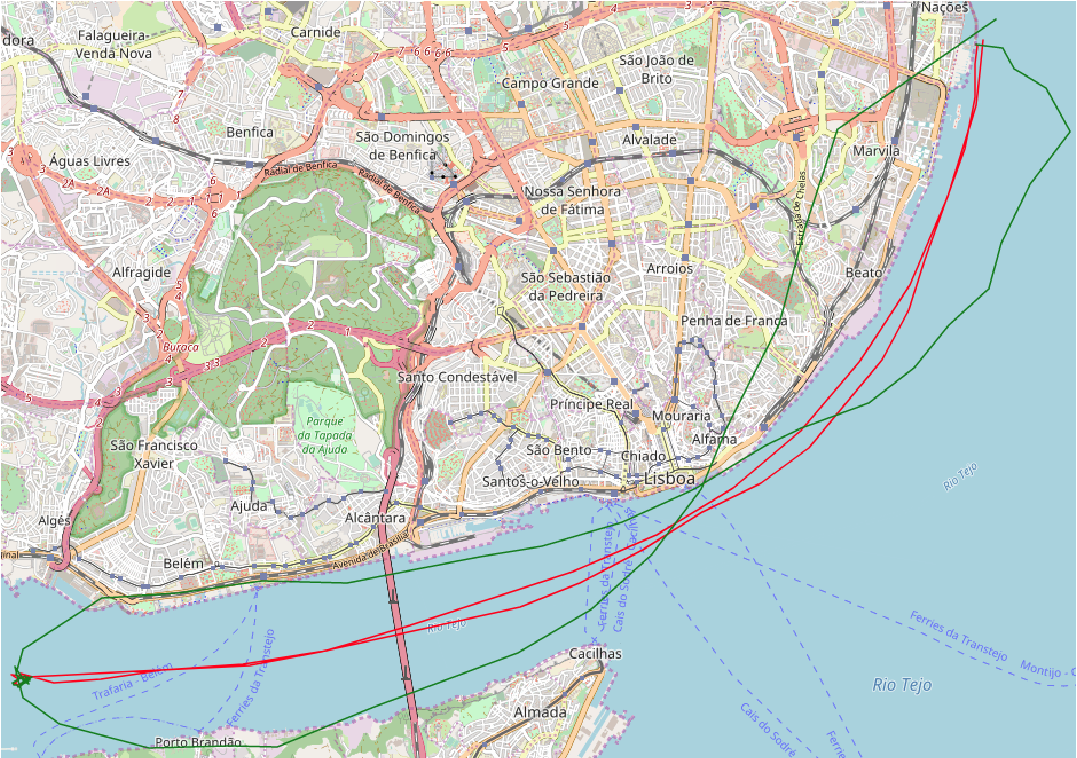
\includegraphics[scale = 0.75]{figures/Ch5/SMM_Estimation_Croped.pdf}
    \caption{Linear Trajectory estimation (Green), applied to the Vessel Trajectory (Red) presented in Section~\ref{subsection: Trajectory Definition}.}
    \label{fig: Chapter 5 SMM linear estimation}
\end{figure}
For any historical trajectory it is possible to know where the was each for every transmission, by calculating the haversine distance between the estimated position at $T^{-1}$ and the actual vessel position at time $T$. This distance represents the distance estimation error. For this trajectory which length was of $138$ $BPs$, the mean distance estimation error was of \textbf{361 meters}. This result for this trajectory were suboptimal, as firstly a Vessel position should never be estimated to be in land, and secondly this specific trajectory had $98$ $BPs$ with a reported $SOG$ under 1knot. Despite all, the presented sub-esperiment, serves as a baseline, for the implementation of more advanced trajectory estimation mehtods as we will discuss in Future Work,~\ref{chapter:Chapter6}.

\subsection{ADS - Navigational Status Validation Experiment}
\label{subsection: ADS - Navigational Status Experiment}
The Navigational Status Validation Experiment, was conducted with similar approach as the Experiment~\ref{subsection: ADS - Rendezvous Experiment}.
This experiment, started with the analysis of the usage frequency of each Navigational Status, as it is presented under in Table~\ref{Table: 5 Status Counts}.
\begin{table}[H]
\centering
\caption{Navigational Status Counts, where the \% is rounded to two decimal places.}
\label{Table: 5 Status Counts}
\begin{tabular}{@{}ccc@{}}
\toprule
Navigational Status & Count & Count(\%) \\ \midrule
0 & 8,895,694 & 52\% \\
15 & 5,334,804 & 31\% \\
5 & 1,030,712 & 6\% \\
7 & 1,012,271 & 6\% \\
3 & 391,141 & 2\% \\
1 & 177,925 & 1\% \\
8 & 71,664 & 0.0\% \\
2 & 23,306 & 0.0\% \\
6 & 14,955 & 0.0\% \\
4 & 62 & 0.0\% \\ \bottomrule
\end{tabular}
\end{table}

In Table~\ref{Table: 5 Status Counts} what is possible to notice is that the distribution of the reported navigational status is extremely skewed. With approximately $83\%$ of all the analysed $BPs$ were reported as either Status 0(Under Way Using Engine) or 15(Default State). 
Despite this skewed distribution, the experiment was still conduced for the statuses that were quantifiable in a stopped or moving expert label, which was explained in Section~\ref{subsection: 4 Navigational Status Validation}. 
This ultimately reduced the $BPs$ which were evaluated by this experiment. Nevertheless the experiment was conducted with $10.1$ Million $BPs$, where the results under in Table~\ref{Table: 5 Status Results}.
%which limited reduced the  Experiment and as described in Section XX, we validated the Navigational Statuses that could be described in a Stopped or Moving kinematic label.  The skewed distribution of the Navigational Status reported in this Data-Set, allowed this validation to be done for the major part of this Data-Set. We were able to validate, validate XXMILION MESSAGES XXPERCENTAGE...
  
\begin{table}[H]
\centering
\caption{Results for Navigational Status Validation Experiment, with the Stopped or Moving approach. }
\label{Table: 5 Status Results}
\begin{tabular}{@{}lllc@{}}
\toprule
Navigational Status & Count & Incoherent Count & Incoherent \% \\ \midrule
0 (using engine) & 8,895,694 & 5225362 & 58.74\% \\
1 (at anchor) & 177,925 & 54,085 & 30.40\% \\
5 (moored) & 1,030,712 & 246,430 & 23.91\% \\
6 (aground) & 14,955 & 2,091 & 13.98\% \\
8 (sailing) & 71,664 & 24,607 & 34.34\% \\
Total & 10,190,950 & 5,552,575 & 54.49\% \\ \bottomrule
\end{tabular}
\end{table}

From the results presented above, it is clear that the major part of the used Navigational Statuses were reported wrongly. Similar results were found in~\cite{Machado2019VesselOutliers}, using a different dataset. A possible reason for such high number of miss used navigational status, might be justified by the fact that the Navigational Status is set by the crew on the AIS device. 
Although to try to better understand this results we started by analysing the areas where the miss-use of navigational status would occur. This analysis is presented in the form of a density plot, which was done using the same packages, as in Experiment~\ref{section: Experiment Data}.

\begin{figure}[H]
	\centering
	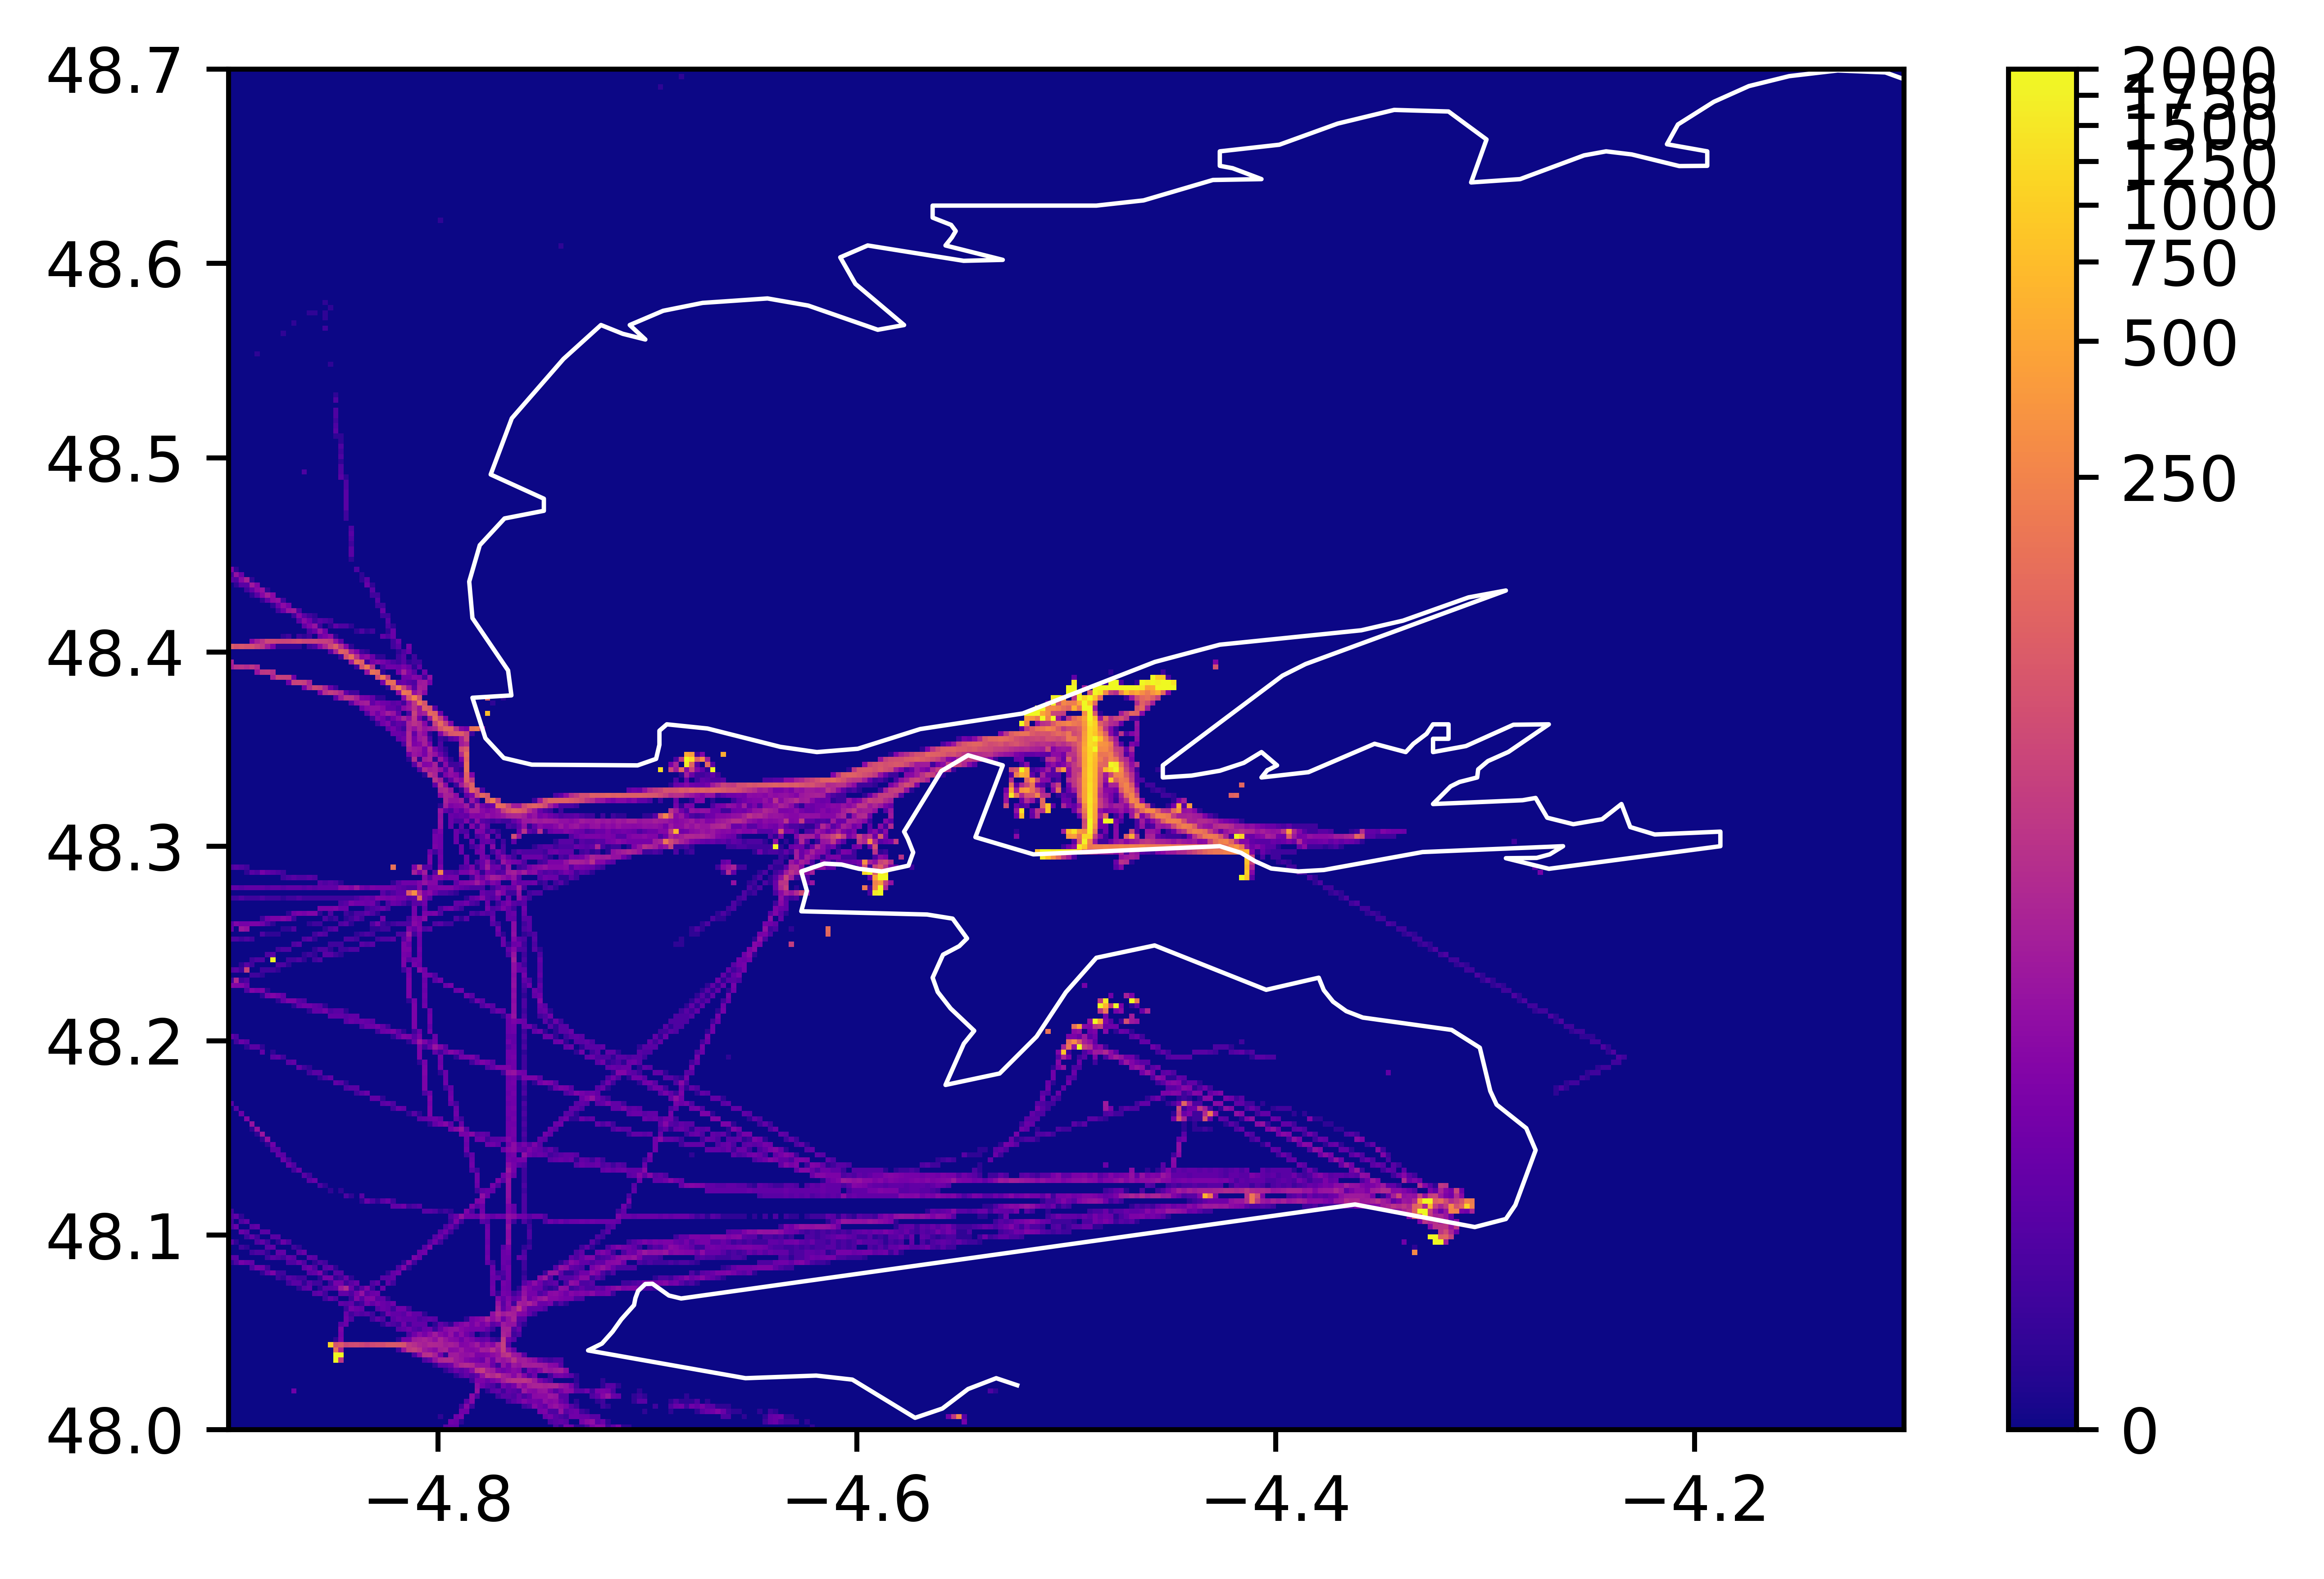
\includegraphics[width=\textwidth]{figures/Ch5/ThesisExpStatusDensityZoom.png}
    \caption{Density map, with all the 5,5M occurrences of wrong Navigational Status.}
    \label{fig: 5 Exp StatusDensityMap}
\end{figure}

What we were able to notice in Figure~\ref{fig: 5 Exp StatusDensityMap}, is that the high density areas where the Navigational Status is reported wrongly, are areas really close to port. As the AIS navigational status needs to be changed each time the vessel arrives at port. This led us to believe that the crew members "forgets" to change the navigational status, while in port. Which is then represented on the data, as the Vessel being stopped on port for long periods of time with the navigational status 0(under way using engine). 

\subsubsection{ADS - Fishing Status Validation Experiment}
\label{subsection: ch5 fishing validation}
Fishing status validation is a sub-Experiment related to the Experiment presented above. As to the best of our knowledge there are no current \emph{public} classified fishing trajectories datasets, the approach taken to validate the usage of this specific status was merely by our analysis. What we done for this sup-Experiment, was the usage of the already pre-defined Gaussian Mix Model presented in Section~\ref{subsection: Fishing Activity Detection}. The model was applied on the sub-set of $BPs$ which had the AIS navigational status reported as \textbf{7 - engaged in fishing}. Despite the acknowledged generalisation and the limited validation of the presented model the presented results serve as our first steps towards the implementation of a MAD-F \emph{fishing detection module}. This will be discusses for future work in Chapter~\ref{chapter:Chapter6}. 

For this sub-experiment we first provide an exploratory analysis of the reported $BPs$ and what would be expected to be reported from fishing vessels. From approximately 3 million $BPs$, transmitted by the fishing vessels (vessel type 30) only about 30\% was in fact transmitted with the navigational status 7(engaged at fishing), as the rest half of them were reported with the default AIS status and as we present in Table~\ref{Table : 5 Fishing Status Counts}. 

\begin{table}[H]
\centering
\caption{Fishing Vessels, Navigational Status Counts, where the \% is rounded to two decimal places.}
\label{Table : 5 Fishing Status Counts}
\begin{tabular}{@{}ccc@{}}
\toprule
Navigational Status & Count & Count(\%) \\ \midrule
15 & 1,290,264 & 0.42 \\
7 & 919,515 & 0.30 \\
0 & 749,419 & 0.25 \\
3 & 37,092 & 0.01 \\
5 & 25,505 & 0.01 \\
8 & 6,394 & 0.00 \\
2 & 2,164 & 0.00 \\
6 & 2,055 & 0.00 \\
1 & 19 & 0.00 \\ \bottomrule
\end{tabular}
\end{table}

We further analysed the transmitted navigational status by analysing, if weather any other vessels had transmitted the engaged at fishing navigational status. As presented under in Table~\ref{Table : 5 Fishing Vessel Type}, we noticed that approximately 10\% of the reported $BPs$ were in fact transmitted by other types of Vessel.

\begin{table}[H]
\centering
\caption{Vessel types which had reported the engaged at fishing navigational status.}
\label{Table : 5 Fishing Vessel Type}
\begin{tabular}{@{}lcl@{}}
\toprule
Vessel Type & Vessel Type Nº & Count \\ \midrule
Fishing Vessel & 30 & 919,515 \\
Other & 90 & 92,576 \\ \bottomrule
\end{tabular}
\end{table}

After this initial analysis, we applied a fishing navigational status validation, by classifying the reported engaged at fishing $BPs$ into a steaming (high speed) or fishing (low speed). From this results we further analyse this classification by comparing this results with the mean speed average, from each group, as we present under in Table~\ref{table: ch5 GMM}.

\begin{table}[H]
\centering
\caption{Fishing, not Fishing classification using the Gaussian Mix Module.}
\label{table: ch5 GMM}
\begin{tabular}{@{}lcc@{}}
\toprule
Label       & Count     & Mean SOG \\ \midrule
Fishing     & 1,552,816 & 6.89   \\
Not Fishing & 1,487,490 & 2.60   \\
Total       & 3,040,306 & 8.72   \\ \bottomrule
\end{tabular}
\end{table}

\section{Marisa Validation Trials}
\label{Section: 5 Marisa Validation}

This section presents how the validation of the developed MAD-F will be processed. The evaluation presented above serves as our own analysis and examination of the results produced by the developed MAD-F. Even though the present work was developed in a highly collaborative spirit, the results used must be evaluated under the project context in order for any method to be truly validated. In \textsc{Marisa}, this is achieved by including the different partners into what was defined in the project as \textbf{Trials}. A Trial represents a defined operational scenario where the project end-users will test the developed \textsc{Marisa} services. Despite the intermediate validation procedures applied throughout this work, the ultimate validation of the developed MAD-F is solely conditional on the performance 
of the project trials. By aggregating the users by region of activity, five different trials were defined for the \textsc{Marisa} Project and they will take place until the end of $2018$. \textsc{Inov} will be present in three of these Trials. For 
the purpose of the present work, we shall describe the Trial for which \textsc{Inov} contributed the most for the preparation of the Iberian Trial. The Iberian Trial will be conducted by the Portuguese Navy and the Spanish Guarda Civil, and will involve \textsc{Inov} and numerous other project partners. This will occur during the first fortnight of November, around the region of the Algarve (Portugal), as shown in Figure~\ref{fig: 5 TrialArea}.  

\begin{figure}[H]
	\centering
	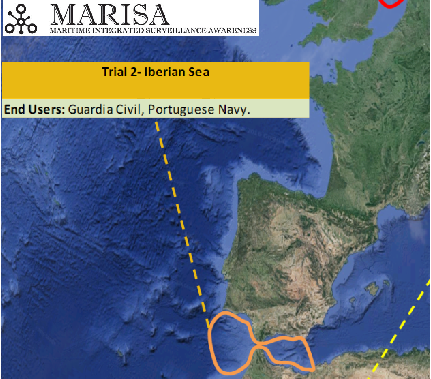
\includegraphics[scale=1.4]{figures/Ch5/IberainTrial.pdf}
    \caption{\textsc{Marisa} Iberian Trial operational area.}
    \label{fig: 5 TrialArea}
\end{figure}

\textsc{Inov} was present in previous meetings with the Portuguese Navy, where the overall execution of the Iberian Trial was discussed. Within the scope of this work's efforts, we are currently ready and able to correlate the Trial activities with the effective validation of the Services and thus the MAD-F. The Iberian Trial will be conducted with real assets, including military vessels from both the Portuguese Navy and the Spanish Guarda Civil, the end-users of this project. Maritime Agents will perform a somewhat choreographed set of vessel manoeuvres able to trigger anomalies. In Table~\ref{Table: Ch5 Trial}, we present the choreography exercise, which will be performed by the Maritime Agents, and how they are correlated with the developed  MAD-F (more specifically by correlating with the Anomaly Requirements which were presented in Section~\ref{section: Framework Requirements}). 
\begin{table}[H]
\centering
\caption{Part of the Choreography conducted for the Iberian Trial. Where V1 and V2 represent a vessel from each end-user, and OC the Operation Control.}
\label{Table: Ch5 Trial}
\resizebox{\textwidth}{!}{%
\begin{tabular}{@{}lll@{}}
\toprule
Provided Description & Choreography & Remarks \\ \midrule
COMMCHECKS & \begin{tabular}[c]{@{}l@{}}at 1000:\\ - OC - communications checks.\end{tabular} &  \\ \midrule
\begin{tabular}[c]{@{}l@{}}TRANSIT TO \\ HIGH SEA\end{tabular} & \begin{tabular}[c]{@{}l@{}}at 1100:\\ - V1 - turns to portside 40º, heading to 140º\end{tabular} &  \\ \midrule
\begin{tabular}[c]{@{}l@{}}TRANSIT TO \\ HIGH SEA\end{tabular} & \begin{tabular}[c]{@{}l@{}}at 1130:\\ - V1 - turns to starboard side 40º, heading to 180º\\ - V1 - increases speed to 25KTS and maintains for 10min.\end{tabular} & \begin{tabular}[c]{@{}l@{}}Aim is to detect Change in  \\ Course Over Ground (COG) and\\ Speed Over Ground (COG).\end{tabular} \\ \midrule
\begin{tabular}[c]{@{}l@{}}TRANSIT TO \\ HIGH SEA\end{tabular} & \begin{tabular}[c]{@{}l@{}}at 1200:\\ - V1 - Turns the AIS System from 1200 to 1220.\\ - OC - Checks if it is detected a change in the AIS System.\end{tabular} & \begin{tabular}[c]{@{}l@{}}Aim is to detect \\ non-broadcasting (AIS)\end{tabular} \\ \midrule
RENDEZVOUS & \begin{tabular}[c]{@{}l@{}}at 1230:\\ - V2 - approaches towards P1(TBD).\\ - V2 - approaches towards P1(TBD).\end{tabular} &  \\ \midrule
RENDEZVOUS & \begin{tabular}[c]{@{}l@{}}at 1300:\\ - V1 - stops at P1 for more than 5min.\\ - V2 - stops at P1 for more than 5min.\end{tabular} & \begin{tabular}[c]{@{}l@{}}Aims to detect the \\ repeated rendezvous \\ of 2 Vessels.\end{tabular} \\ \midrule
\begin{tabular}[c]{@{}l@{}}TRANSIT ALONG \\ SIDE COASTLINE\end{tabular} & \begin{tabular}[c]{@{}l@{}}at 1400:\\ - OC - manipulates the V1 and V2 AIS signal.\\ - V1  - heads to port.\\ - V2  - heads to port.\end{tabular} & \begin{tabular}[c]{@{}l@{}}Aims to detect \\ Incoherent Position and \\ Navigational Status.\end{tabular} \\ \bottomrule
\end{tabular}%
}
\end{table}

The choreography exercise just detailed, within the greater scope of the Iberian Trial, will test conclusively the capabilities of our methodologies. It is worth mentioning that a large portion of Data Science projects suffer from either absent or weak validation stages. This project, in turn, relies on actual, verifiable validation schemes which were devised and coordinated appropriately, given the excellent collaboration links provided by the \textsc{Marisa} project.
\chapter{Conclusion and Future Work}
\label{chapter:Chapter6}
\lhead{Chapter 6. \emph{Conclusion and Future Work}}

In summary, this work is concerned with the detection and identification of anomalies at seas. This task in itself, as was discussed throughout this work, is rather complex and can only be meaningful when a suitable definition of anomaly is applied to the problem at hand. Without such particular constraints, both the aim and eventual conclusions become of general scope. Greatly justified by this reason, we were fortunate to have discussed these technicalities with Maritime experts via the \textsc{Marisa} project. Their insights and feedback lead to a workable interaction level which ultimately allowed us for the development of a number of data-driven methods to be applied, 
resulting in our MAD-F. 

The implemented MAD-F which was developed in accordance with the defined objectives presented in Section~\ref{section: thesis objectives} is able to ingest and process high throughputs of real maritime data. This was achieved with our selection of technologies, namely Python's Pandas package and Apache's Kafka stream processing platform. This provided, generally speaking, a very effective and flexible framework to handle and structure the data. Despite the fact that these tools render the Framework modular and hence scalable, we believe improvements could be achieved by using Apache's Spark cluster-computing framework.

Regarding the transformation of the data into sequential form, we introduced the concept of Behavioural Point $BP$, with which the maritime data features were transformed as to become more suitable for further manipulation. The output data at this stage serves as the adequate input for applying the Anomaly Detection.
The AD modules implemented for the current MAD-F are rule-based, as opposed to more sophisticated methods. Despite the ever-growing demand for far more complex and involved methodologies, this procedure still yields very satisfactory results. 

There are many reasons for choosing this procedure. Firstly, no publicly-available classified datasets exist for this source of data, to the best of our knowledge. This invariably forbids us from labelling anomalies without the explicit guidance of experts in the field. Secondly, applying more sophisticated methods requires a longer project execution time, which was a delicate issue from the outset. 
In spite of all these reasons presented above, we are confident the Framework is easily scalable for future development and offers an easy integration of new modules in the future. 

\textsc{Marisa} is admittedly an ambitious endeavour which takes in contributions from multiple partners from all around Europe, as well as institutional agencies of different countries. Progress in highly technical matters is therefore inevitably slower than what would be expected from smaller projects.

It is our intention to look into new modules to complement and further expand the scope of this Framework. The linear estimation of the vessel trajectories used in our framework would benefit greatly by employing more intricate estimation methods such as Kalman filter~\cite{Borkowski2017TheFusion, Perera2012MaritimePrediction}. An explicit module for detection of fishing activity, as discussed at length by the Global Fish Watch project~\footnote{http://globalfishingwatch.org/publications/}, would bring added value to the Framework. Lastly, the study of the vessel trajectories, which was based on a point-based analysis up to now, could be upgraded to a time series analysis. Related procedures such as multivariate time series clustering, already mentioned in the state of art in Subsection,~\ref{section: ch2 timeseriesclassification} and~\ref{section: ch2 timeseriesclustering}.  

Additionally, some modules from the developed \textsc{Modular Anomaly Detection Framework}, originated the work~\cite{Machado2019VesselOutliers}, which provided a particular emphasis on the detection of the Rendezvous anomaly detection.
%\chapter{DUMP} %This was made for FCD subject, 2306 -> this is old... 

%\todo[inline]{annotations +  table different sources of data bases}
The initial AIS database was created from a open-source AIS provided by U.S. coastal waters, ~\cite{MarineCadastre}. The raw database file dbf was downloaded, and transformed to a csv, with the use of a open-source GIS software (QGIS). 
 
Before the download of the data-set it was important to select one area of more interest, as dbf to csv transformations are time consuming, and the a decent sized data-set, was achieved with just one area.

\begin{figure}[H]
	\centering
	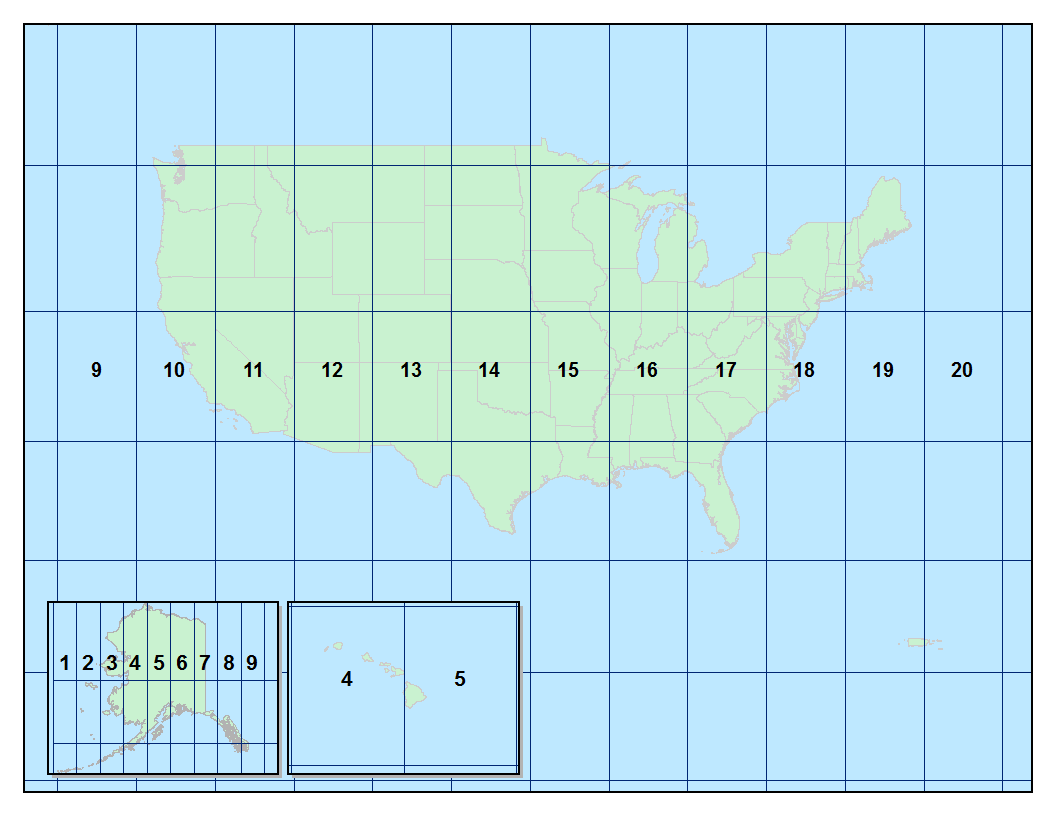
\includegraphics[scale = .35]{figures/UTMZoneMap2014.png}
    \caption{Index map of UTM zones}
    \label{fig: UMT zones}
\end{figure}

The initial selected zone, was zone 10. This zone represents the west coast of the United States, as it is shown in Figure ~\ref{fig: UMT zones}.
The chosen area, represents data whose longitude is from -120 to -126 and latitude is from 30 to 50, from a considerable amount of ships.

%http://www.marinecadastre.gov/ais/

\section{AIS Data}
 With the recent introduction of AIS in the Maritime domain the volume of vessel positional data as exponentially increased, a detailed description of this data, is found in section ~\ref{subsection: chp2_AIS}.

\begin{table}[H]
\centering
{\small
\begin{tabular}{lrrrrrl}
\toprule
{} &       MMSI &           X &          Y &   SOG &        COG &                Time \\
\midrule
0 &  636081210 & -125.993218 &  48.355773 &  14.3 &  73.300003 & 2014-02-27 13:33:02 \\
1 &  636081210 & -125.985303 &  48.357340 &  14.5 &  73.800003 & 2014-02-27 13:34:23 \\
2 &  636081210 & -125.979437 &  48.358500 &  14.6 &  73.099998 & 2014-02-27 13:35:23 \\
3 &  636081210 & -125.973353 &  48.359692 &  14.7 &  73.000000 & 2014-02-27 13:36:25 \\
4 &  636081210 & -125.965440 &  48.361318 &  15.0 &  73.000000 & 2014-02-27 13:37:46 \\
5 &  636081210 & -125.956733 &  48.363067 &  15.3 &  73.900002 & 2014-02-27 13:39:11 \\
6 &  636081210 & -125.950430 &  48.364153 &  15.7 &  76.099998 & 2014-02-27 13:40:11 \\
7 &  636081210 & -125.944108 &  48.365310 &  15.7 &  74.000000 & 2014-02-27 13:41:10 \\
8 &  636081210 & -125.937763 &  48.366510 &  15.9 &  73.900002 & 2014-02-27 13:42:12 \\
9 &  636081210 & -125.931385 &  48.367660 &  15.9 &  75.000000 & 2014-02-27 13:43:11 \\
\bottomrule
\end{tabular} }
\caption{Example of AIS data transmitted by Vessel, MMSI: 636081210}
\label{Table: TableAIS1}
\end{table}


\section{Route Representation}
Representing the data of a Vessel trajectory, can become a difficulty in the Maritime domain. There are a vast number of techniques described in the literature.

A effective way to represent a trajectory in the Maritime domain, is to look to the trajectory as a whole, this is, as vessel are obliged to broadcast their AIS information in a semi-continuous rates; knowing that each AIS broadcast message represent the instantaneous kinematic information from a single vessel, aggregating this information over time will represent a vessel trajectory. Therefore, knowing the MMSI of a vessel, a trajectory can be considered as the set of AIS messages broadcast, by that vessel, identified by the MMSI.


Thus, a possible definition for a vessel trajectory is a, set of multidimensional-points represented as:
\[TR_{MMSI} = p1, p2, p3, p4, \cdots , pn\]

Where each multidimensional point $p$ is defined as:
\[p = [t, x, y, SoG, CoG]\]


%\todo[inline]{ TODO SE FALTAR DADAS A INTERPOLAÇAO REALIZADA}


%for the Representation of MMSI as a track initially, then the assumption... interpolation of missing SOG and COG values. The use of Haversine formula, justify with as vessel motion is linear and no sudden speed exchanges or route exchanges tend to occur in secounds in the marite traffic, so this .

\section{MARISA Requirements}

\addtocontents{toc}{\vspace{2em}}

%-------ANEXOS---------

%\appendix
%\appendixpage
%\addappheadtotoc

%\chapter{Appendix's title}
%\label{AppendixA}
%\lhead{Appendix A. \emph{Appendix's title}}


\addtocontents{toc}{\vspace{2em}}
\backmatter

%-------BIBLIOGRAFIA---------
%Adicionem as referências em BibTeX ao ficheiro references.bib
\label{References}
\lhead{\emph{References}} 
 
%\bibliographystyle{plain}
%\bibliographystyle{ieeetr}
%\bibliographystyle{ieeetr}

\bibliographystyle{ieeetr}
%\bibliography{ThesisReferences}
\bibliography{references}

\end{document}